\documentclass[12pt,a4paper,openright,twoside]{report}
\usepackage{geometry}
\usepackage[english]{babel}
\usepackage[latin1]{inputenc}
\usepackage{fancyhdr}
\usepackage{indentfirst}
\usepackage{graphicx}
\usepackage{subcaption}
\usepackage{newlfont}
\usepackage{amssymb}
\usepackage{amsmath}
\usepackage{latexsym}
\usepackage{amsthm}
\usepackage{booktabs}
\usepackage{array}
\usepackage{braket}
\hyphenation{sil-la-ba-zio-ne pa-ren-te-si}
\pagestyle{fancy}\addtolength{\headwidth}{20pt}
\renewcommand{\chaptermark}[1]{\markboth{\thechapter.\ #1}{}}
\renewcommand{\sectionmark}[1]{\markright{\thesection \ #1}{}}
\rhead[\fancyplain{}{\bfseries\leftmark}]{\fancyplain{}{\bfseries\thepage}}
\cfoot{}

\begin{document}
	
\newgeometry{margin=1in}
\begin{titlepage}
		\begin{center}
			{{\Large{\textsc{Alma Mater Studiorum $\cdot$ Universit\`a di
							Bologna}}}} \rule[0.1cm]{15.8cm}{0.1mm}
			\rule[0.5cm]{15.8cm}{0.6mm}
			{\small{\bf SCUOLA DI SCIENZE\\
					Corso di Laurea in Fisica Nucleare e Subnucleare }}
		\end{center}
		\vspace{15mm}
		\begin{center}
			{\LARGE{\bf Monitoring of the DUNE}}\\
			\vspace{3mm}
			{\LARGE{\bf Long Baseline Neutrino Beam}}\\
			\vspace{3mm}
			{\LARGE{\bf with the SAND Detector}}\\
		\end{center}
		\vspace{40mm}
		\par
		\noindent
		\begin{minipage}[t]{0.4\textwidth}
			{\large{\bf Relatore:\\
					Prof. Sergio Bertolucci\\ \\
				    Correlatore:\\
			        Dott. Matteo Tenti}}
		\end{minipage}
		\hfill
		\begin{minipage}[t]{0.4\textwidth}\raggedleft
			{\large{\bf Presentata da:\\
					Federico Battisti}}
		\end{minipage}
		\vspace{30mm}
		\begin{center}
			{\large{\bf Sessione III\\ 
					Anno Accademico 2018-2019}}%inserire l'anno accademico a cui si � iscritti
		\end{center}
	\end{titlepage}
                       
\restoregeometry


\begin{titlepage}                      
\thispagestyle{empty}                  
\topmargin=6.5cm                        
\raggedleft                            
\large                                  
\em                                    
``I have done a terrible thing:\\
 I have postulated a particle that cannot be detected'' \\ 
 Wolfgang Pauli                      
\newpage                               
\clearpage{\pagestyle{empty}\cleardoublepage}
\end{titlepage}




\pagenumbering{roman}                   
\tableofcontents                       
\rhead[\fancyplain{}{\bfseries\leftmark}]{\fancyplain{}{\bfseries\thepage}}
\lhead[\fancyplain{}{\bfseries\thepage}]{\fancyplain{}{\bfseries CONTENTS}}

\clearpage{\pagestyle{empty}\cleardoublepage}

\chapter*{Abstract}
\rhead[\fancyplain{}{\bfseries Abstract}]{\fancyplain{}{\bfseries\thepage}}
\lhead[\fancyplain{}{\bfseries\thepage}]{\fancyplain{}{\bfseries Abstract}}
\addcontentsline{toc}{chapter}{Abstract}
The Deep Underground Neutrino Experiment (DUNE) will be a next generation neutrino oscillation long baseline accelerator experiment. It will be composed of a Near Detector (ND) system located a few hundred meters from the neutrino source at Fermilab, and a Far Detector (FD) system composed of four multi-kiloton LArTPCs. Of the three Near Detectors, SAND (System for on-Axis Neutrino Detection) will have as its main purpose to provide constraints on all the systematic uncertainties relevant for the oscillation analysis. Among these, one of the detector's main task will be beam monitoring which consists in using the flux measurements to spot potential anomalies in the beam production. This thesis studies the beam monitoring capabilities of the SAND detector, via neutrino flux and detector simulations.
\clearpage
\chapter*{Sommario}
Il Deep Underground Neutrino Experiment (DUNE) sar� un esperimento sull' oscillazione di neutrini da acceleratore da ``long baseline" di nuova generazione. Sar� composto da un sistema di Near Detector (ND) posizionato a poche centinaia di metri dalla fonte di neutrini al Fermilab, a un sistema di Far Detector (FD) composto da quattro LArTPC dell'ordine di dieci migliaia di tonnellate. Dei tre rivelatori che compongono il sistema del Near Detector, SAND (System for on-Axis Neutrino Detection) avr� come sua funzione principale quella di ridurre le incertezze sistematiche che interessano le misure di oscillazione di neutrini. Tra queste, una delle principali funzioni del detector sar� il beam monitoring, che consiste nell'identificare eventuali variazioni del flusso di neutrini legate ad anomalie nella produzione del fascio. Questa tesi ha lo scopo di studiare le capacit� di monitoring del fascio del rivelatore SAND, tramite simulazioni del flusso di neutrini, dei detector e della loro risposta al passaggio delle particelle. 
\clearpage
\chapter*{Introduction}                 
%%%%%%%%%%%%%%%%%%%%%%%%%%%%%%%%%%%%%%%%%imposta l'intestazione di pagina
\rhead[\fancyplain{}{\bfseries Introduction}]{\fancyplain{}{\bfseries\thepage}}
\lhead[\fancyplain{}{\bfseries\thepage}]{\fancyplain{}{\bfseries Introduction}}
\addcontentsline{toc}{chapter}{Introduction}
Since their discovery neutrino oscillations have become one of the most direct evidence of the fact that the Standard Model of particle physics is not a complete theory. Many of the parameters that govern the phenomenon have been accurately measured by a variety of experiments, exploiting either the solar and atmospheric neutrino fluxes or artificial ones produced by nuclear reactors or particle accelerators. \\
The Deep Underground Neutrino Experiment (DUNE) will be a next generation neutrino oscillation Long Baseline accelerator experiment. The experiment is set to reach new levels of precision, allowing for the first time a definitive measurement of the possible neutrino oscillation CP-violation and of the neutrino mass ordering. \\
The DUNE experiment will be composed of a Near Detector (ND) system located a few hundred meters from the neutrino source at Fermilab, and a Far Detector (FD) system composed of four multi-kiloton Liquid Argon Time Projection Chambers (LArTPC) located at 1300 km from the source. The ND system will be composed of three individual detectors: ArgonCube, HPgTPC (High Pressure gas TPC) and SAND (System for on-Axis Neutrino Detection). While the first two are both based on Argon technologies, the SAND design considered in this thesis (one of a few still in consideration) will take a totally different approach by implementing a modular Straw Tube Tracker (STT), integrating many different nuclear targets. SAND will also be the only detector in DUNE to re-use parts from an older detector: it will implement the electro-magnetic calorimeter, magnet and iron structure from the KLOE (K-LOng Experiment) detector. \\
SAND's main purpose will be to provide constraints on all the systematic uncertainties relevant for the oscillation analysis. These include measurements of interaction cross sections, physics and detector responses and neutrino flux spectrum, composition and spread.\\
One of SAND's main tasks will be beam monitoring, which consists in using the flux information from the ND measurements to spot potential anomalies in the beam production. The purpose of this thesis is to study the beam monitoring capabilities of the SAND detector, via neutrino flux and detector simulations. The text is divided into five chapters:
\begin{itemize}
	\item \emph{Chapter 1}: Summary of the history of neutrino physics and its future prospects, and brief theoretical overview of the neutrino oscillation phenomenon; 
	\item \emph{Chapter 2}: Description of the DUNE experiment's components and facilities and its physics goals; 
	\item \emph{Chapter 3}: Description of the SAND detector and its main purposes and experimental physics opportunities;
	\item \emph{Chapter 4}: Overview of the software and data used for the DUNE neutrino flux and detector simulations;
	\item \emph{Chapter 5}: Description, analysis and results of the beam monitoring study;
\end{itemize}
\clearpage{\pagestyle{empty}\cleardoublepage}

\chapter{Neutrino physics overview}                
\rhead[\fancyplain{}{\bfseries Chapter 1: Neutrino physics overview}]{\fancyplain{}{\bfseries\thepage}}
\lhead[\fancyplain{}{\bfseries\thepage}]{\fancyplain{}{\bfseries Chapter 1: Neutrino physics overview}}
\pagenumbering{arabic}           \label{chapter 1}   
\section{Brief history of neutrinos}
\label{sec:neutrino history}
Neutrinos made their first appearance in modern physics as an hypothetical particle proposed by W. Pauli in order to solve the problem related to the continuous energy spectrum measured for $\beta$-decay electrons  \cite{Pauli}. It was given its name by Enrico Fermi, the first to develop a theory of beta decay that included the new particle as one of the four fermions involved in the correspondent interaction \cite{Fermi}. Fermi's theory led Bethe and Peierls to the first estimation of the inverse interaction's cross section \cite{Bethe-Peierls}:
\begin{equation}
\sigma(\bar{\nu}p\rightarrow ne^+)\leq 10^{-44} \ \text{cm}^2, \ \ E_{\bar{\nu}}\simeq 2 \text{MeV} 
\end{equation}
The smallness of the cross section led the two scientists to conclude that it would be almost impossible to detect such an interaction. \\
B. Pontecorvo was the first to realize that with a neutrino flux of about $10^{11}\nu/\text{cm}^2/\text{s}$, of the order of the one produced by an average nuclear reactor, and a ton mass scale detector one could obtain a rate of a few events per day \cite{Pontecorvo}. This idea was put into practice by Reines and Cowan, whose experiment led to the discovery of the anti-neutrino in 1956 \cite{Reines-Cowan}. Their technique for the identification of the antineutrino inverse beta decay interactions relied on the detection of the light produced by the neutron capture, in delay with respect to the annihilation of the positron, a signature still in use today. \\
In 1962 Lederman, Schwarts and Steinberger showed the existence of a second type of neutrino, associated with the muon in the main decay mode of the pion: $\pi ^- \rightarrow \mu^-\bar{\nu_\mu} $ \cite{Lederman-Misty-Steinberg}. This was also the first case in which an accelerator neutrino beam was used in any experiment. Such beam was generated by the decay of pions and other hadrons produced in the collision of accelerated protons on a target. A neutrino detector revealed the leptons produced in the charged current (CC) interactions.\\
The $\tau$ lepton was discovered at the SLAC accelerator in the seventies, and it would soon be argued that a third neutrino might be associated to it as for the lighter leptons. The study of the decay width of the $Z_0$ produced at LEP in $e^+e^-$ collisions showed that the number of light neutrinos coupled to the neutral weak boson was three (Fig. 1.1 ) \cite{LEP}:
\begin{equation}
N_\nu=\frac{\Gamma_{inv}}{\Gamma_{\bar{\nu}\nu}} = 2.984\pm 0.008
\end{equation}
\begin{figure}
	\centering
	\label{LEPnu-fig}
	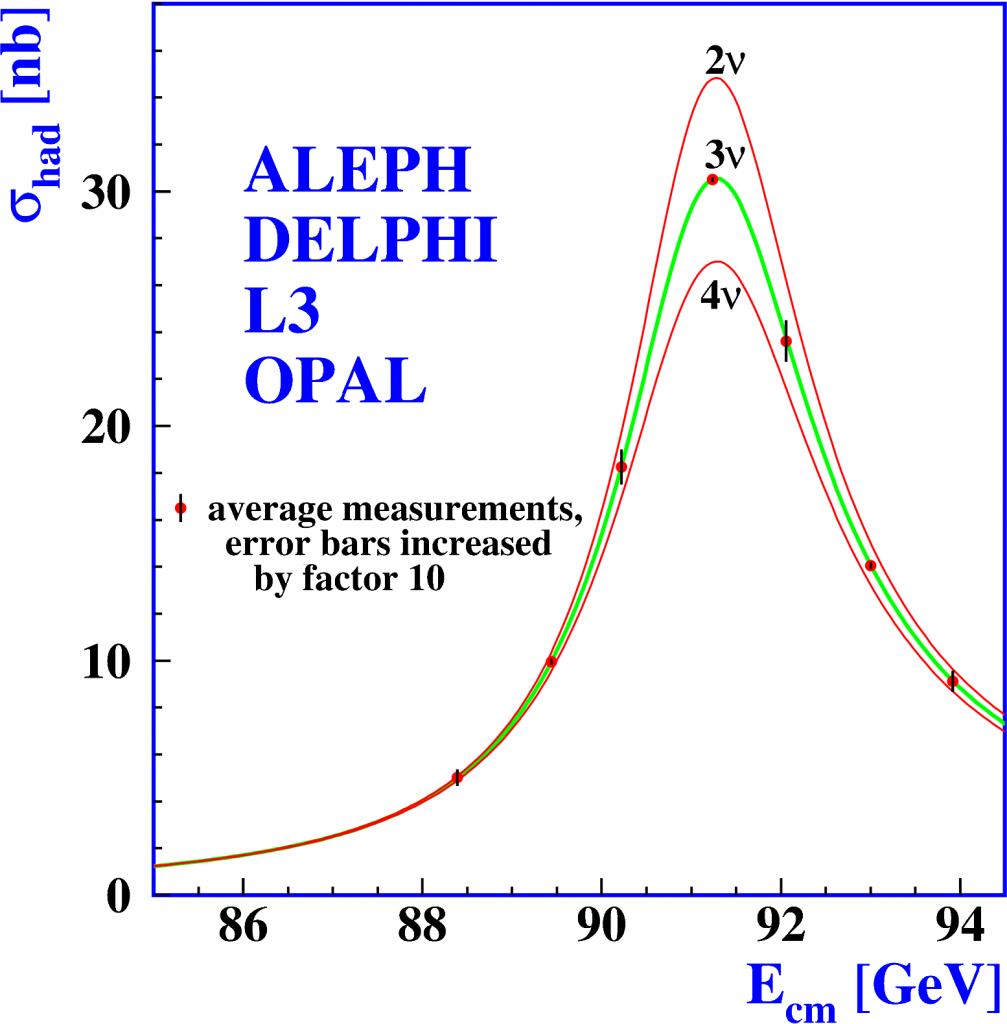
\includegraphics[width=0.5\textwidth]{LEP-NuFlavours.png}
	\caption{Theoretical predictions of the total cross-section for
		the production of hadrons as a function of the center of mass energy for 2, 3 and 4 neutrino families. Experimental data from LEP drawn as dots. \cite{LEP}}
\end{figure}
The tau neutrino was finally discovered at Fermilab in 2001 at the DONUT experiment by revealing the taus produced in CC interactions in iron \cite{DONUT}.
\section{Neutrinos in the Standard Model and neutrino masses}
\label{sec:SM}
The Standard Model (SM) of particle physics is a gauge theory defined by the symmetry $SU(3)\times SU(2)_L \times U(1)_Y$ with the subscripts L and Y indicating the left chirality of the particles and their hypercharge respectively. The $SU(3)$ describes the strong interaction in the quark sector while $SU(2)_L \times U(1)_Y$ is related to the electroweak sector. \\
The particles in the SM are divided into bosons of spin 1 that mediate the fundamental interactions (photons for the electromagnetic interactions, $W^ \pm$ and $Z^0$ for the weak sector and 8 gluons for the strong sector), the spin 0 Higgs boson and the fundamental fermions quarks and leptons, organized in $SU(2)_L$ left-handed doublets and $U(1)_Y$ right handed singlets (see Table \ref{tab:SM}).

\begin{table}[t]
	\centering
	\setlength{\tabcolsep}{8pt}
	\renewcommand{\arraystretch}{1.3}
	\begin{tabular}{ c c | c c c}
		\hline 
		\hline
		$\begin{pmatrix} \nu_e \\ e \end{pmatrix}_L$ & $\begin{pmatrix} u \\ d \end{pmatrix}_L$ & $e_R$ & $u_R$ & $d_R$\\
		$\begin{pmatrix} \nu_\mu \\ \mu \end{pmatrix}_L$ & $\begin{pmatrix} c \\ s \end{pmatrix}_L$ & $\mu_R$ & $c_R$ & $s_R$\\
	$\begin{pmatrix} \nu_\tau \\ \tau \end{pmatrix}_L$ & $\begin{pmatrix} t \\ b \end{pmatrix}_L$ & $\tau_R$ & $t_R$ & $b_R$\\
		\hline\hline
	\end{tabular}
    \caption{\label{tab:SM}All irreducible fermion representations in the the SM.}
\end{table}%
Neutrinos are charge-less fermions that can interact only weakly, either via Neutral Current (NC) interactions mediated via $Z^0$ bosons or Charged Current (CC) via $W^\pm$ bosons. The flavour of the neutrino is simply defined by the charged lepton that is connected to the same charged current vertex:
\begin{equation}
\begin{split}
W^+\rightarrow e^+ + \nu_e\\
   \rightarrow \mu^+ + \nu_\mu\\
   \rightarrow \tau^+ + \nu_\tau
\end{split}
\end{equation}  
The weak interaction is parity violating and only left-handed particles $\nu_L$ or right handed anti-particles $\bar \nu_R$ participate to the interaction. For this reason only left-handed neutrinos and right-handed anti-neutrinos have been introduced in the SM, making it impossible to construct a Dirac mass term:
\begin{equation}
\mathcal{L}^{Dirac}_{mass}=m_D(\bar{\psi}_L\psi_R + \bar{\psi}_R\psi_L), \ \text{with} \ \bar{\psi}_R\psi_L = (\bar{\psi}_L\psi_R)^\dagger 
\end{equation}
where $\psi_{L,(R)}$ is the left(right)-handed chiral component (Weyl spinors). It is obvious that both a left-handed and a right-handed neutrino would have to exist in order to be able to construct a Dirac mass term. On the other hand, as we will discuss more in detail later (see Sec. \ref{sec: Oscillation}), neutrino oscillation phenomena require neutrinos to be massive particles.
\\
One  solution to this problem is to extend the Standard Model to include a right-handed neutrino $\nu_R$ \cite{Lipari}. Since neutrinos are neutral, another possibility is that they are Majorana particles, i.e. neutrino and antineutrino are the same particle. Such a fermion would be described by a single Weyl spinor. A Majorana mass term with a single Weyl-spinor, either left or right handed can then be introduced as:
\begin{equation}
\mathcal{L}^{Majorana}_{mass}=- \frac{m_M}{2}[(\psi_L)^Ti\sigma^2\psi_L+h.c.].
\end{equation}
In principle it is possible to construct both a Dirac and a Majorana term. This could be written as:
\begin{equation}
\mathcal{L}^\nu_{mass}=-\frac{1}{2}(\bar{\psi}_L,\bar{\psi}_L^c) \begin{pmatrix} m_{M,L} & m_D \\ m_D & m_{M,R} \end{pmatrix} \begin{pmatrix} \psi_R^c \\ \psi_R\end{pmatrix}
\end{equation}
where c stands for the the conjugation operation. The Dirac mass term can be expected to be of the same order of the other fermions in the family while the Majorana mass term $m_{M,L}$ should be null to not break $SU(2)_L \times U(1)_Y$ symmetry. Finally a right handed neutrino would be completely neutral under the standard-model gauge-group (i.e $sterile$), and it could have a mass of the order of GUT (Grand Unified Theories) scale ($M\sim 10^{16} \text{GeV}$), without actually breaking any symmetry. The mass matrix could be written as:
\begin{equation}
\mathcal{M}\simeq \begin{pmatrix}
0 & m_D \\
m_D & M
\end{pmatrix}
\end{equation} 
This matrix can be diagonalized to obtain two eigenvalues that are approximately $M$ and $-m_D^2/M$. The two mass eigenvalues correspond to one very massive and sterile ($m_N\simeq M$) and one very light and weakly interacting ($m_\nu\simeq m_D^2/M$). The second particle would correspond to the neutrinos we normally observe. This so-called Type 1 see-saw mechanism is one of the possible explanations for the smallness of the neutrino masses.\\
The main experimental technique used today to confirm whether neutrinos are Majorana particles or more canonical Dirac fermions is the search for the so called neutrino-less double beta decay, a process only possible if neutrinos and antineutrinos are the same particle. Some of the experiments now active in the field now include Gerda, CUORE and CUPID and CANDLES \cite{Petcov}.


\subsection{Limits on neutrino masses}
\label{sec: mass limits}
Even if the neutrino oscillation phenomenon indicates that neutrinos are massive particles, it depends only on the squared mass differences and as such, they can't be used to obtain limits on the mass values. A direct measurement of neutrino masses is possible, in principle, using kinematical methods, though these strategies have only produced upper limits so far.\\
For  $\bar{\nu}_e$ the most effective technique relies on the measurement of the highest kinematically allowed energy in the $\beta$-decay spectrum. Such value is related to the neutrino mass as : $E_{\text{endpoint}}^e\simeq Q -m_\nu$. The best limit is currently set by the KATRIN experiment \cite{KATRIN}, which has recently halved the previous estimates from the Troitsk \cite{Troisk} and Mainz \cite{Mainz} experiments (all study the decay of tritium):

\begin{equation}
\begin{split}
m_{\nu_e} & < 2.05\text{ eV at 95\% C.L. (Troitsk);}\\
          & < 2.3\text{ eV at 95\% C.L. (Mainz);}\\
          & < 1.1\text{ eV at 90\% C.L. (KATRIN);}
\end{split}
\end{equation}
Limits on the masses of the other flavours \cite{PDG} are currently much less stringent and are obtained by studying the pion decay and the $\tau$ decay kinematics for $\nu_\mu$ and $\nu_\tau$ respectively: 
\begin{equation}
\begin{split}
m_{\nu_\mu} & < 170\text{ keV at 90\% C.L. ;}\\
m_{\nu_\tau}& < 18.2\text{ MeV at 95\% C.L. ;}\\
\end{split}
\end{equation}
Limits on the sum of the three masses can also be set by cosmological experiments such as Planck \cite{Planck}. These limits are model dependent and in the Standard Cosmological Model are currently set at:
\begin{equation}
\sum_{j}m_j \leq 0.12 \text{ eV}
\end{equation}
Finally the non observation of neutrino-less double beta decay can set a limit on the electron neutrino effective mass in the case that neutrinos are Majorana particles:
\begin{equation}
\langle m_{\nu_e} \rangle _{eff} \lesssim 0.4 \text{ eV}
\end{equation}

\section{Theory of neutrino oscillations }
\label{sec: Oscillation}
If neutrinos have non-vanishing rest mass, the weak and mass eigenstates are not necessarily the same, a fact that is well known in the quark sector where the CKM matrix connects the two types of states. This makes the phenomenon of neutrino oscillations possible i.e. a neutrino produced with a specific flavour can later be measured to have a different flavour. The experimental discovery of this new behaviour in 1998 is currently the unique evidence that the Standard Model is not a complete theory\cite{Zuber} \cite{Giunti}.\\
\subsection{Three flavours oscillations in vacuum}
The 3 orthonormal flavour eigenstates $\ket{\nu_\alpha}$  (where $\alpha = e, \mu, \tau$) are connected to 3 orthonormal mass eigenstates $\ket{\nu_i}$ via a unitary mixing matrix $U$ \cite{Zuber}:
\begin{equation}
\label{mix:eq}
\ket{\nu_\alpha}=\sum_i U_{\alpha i} \ket{\nu_i} \text{ ;   } \ \ket{\nu_i}=\sum_\alpha U_{\alpha i}^* \ket{\nu_\alpha} \text{ ;  }
\end{equation}
The matrix, in the case of 3 neutrino flavours is the so called PMNS (Pontecorvo-Maki-Nakagawa-Sakata) matrix and can be parametrized as:
\begin{equation}
\begin{split}
U & =
\begin{bmatrix}
1 & 0 & 0 \\
0 & c_{23} & s_{23} \\
0 & -s_{23} & c_{23}
\end{bmatrix}
\quad
\begin{bmatrix}
c_{13} & 0 & s_{13}e^{-i\delta} \\
0 & 1 & 0 \\
-s_{13}e^{i\delta} & 0 & c_{13}
\end{bmatrix}
\quad
\begin{bmatrix}
c_{12} & s_{12} & 0 \\
-s_{12} & c_{12} & 0 \\
0 & 0 & 1
\end{bmatrix} = \\[8pt]
& =
\begin{bmatrix}
c_{12}c_{13} & s_{12}c_{13} & s_{13}e^{-i\delta} \\
-s_{12}-c_{12}s_{23}s_{13}e^{i\delta} & c_{12}c_{23}-s_{12}s_{23}s_{13}e^{i\delta} & s_{23}c_{13} \\
s_{12}s{23}-c_{12}c_{23}s_{13}e^{i\delta} & -c_{12}s_{23}-s_{12}c{23}s_ {13}e^{i\delta} & c_{23}c_{13}
\end{bmatrix}
\end{split}
\end{equation}
\\
where $c_{ij} =\text{cos}\ \theta_{ij}$, $s_{ij} =\sin\theta_{ij}$, $\theta_{ij}$ are the mixing angles and $\delta$ is the Dirac charge-parity (CP) symmetry violating phase. In the case of Majorana neutrinos the matrix contains two additional Majorana phases which appear in a diagonal matrix that multiplies U:
\begin{equation}
U^{Majorana}= 
\begin{bmatrix}
1 & 0 & 0 \\
0 & e^{i\phi_2/2} & 0 \\
0 & 0 & e^{i\phi_3/2}
\end{bmatrix}
\end{equation} 
These additional phases do not affect neutrino oscillations and cannot be measured in neutrino oscillation experiments.\\
The mass eigenstates $\ket{\nu_i}$, being the eigenstates of the Hamiltonian ($\mathcal{H}\ket{\nu_i}=E_i\ket{\nu_i}$) show a time dependence :
\begin{equation}
\label{massev:eq}
\ket{\nu_i(t)}=e^{-iE_it}\ket{\nu_i} 
\end{equation} 
with $E_i=\sqrt{\vec{p} \ ^2+m_i^2}$ in natural units (i.e. $c=1$). If we now consider a flavour state $\ket{\nu_\alpha(t)}$ which represents a neutrino of definite flavour created at t=0 ($\ket{\nu_\alpha(t=0)}=\ket{\nu_\alpha}$), from eq. \ref{mix:eq} and \ref{massev:eq} the time evolution of this state is given by:
\begin{equation}
\begin{split}
\ket{\nu_\alpha(t)} & =\sum_i U_{\alpha i}e^{-iE_it}\ket{\nu_i}\\
                    & =\sum_{\beta} \big(\sum_i U_{\alpha i}^* e^{-iE_it} U_{\beta i}\big) \ket{\nu_\beta}
\end{split}
\end{equation}
The amplitude of the transition $\nu_\alpha \rightarrow \nu_\beta$ is then:
\begin{equation}
\mathcal{A}_{\nu_\alpha \rightarrow \nu_\beta}(t)= \braket{\nu_\beta|\nu_\alpha(t)}=\sum_i U_{\alpha i}^* U_{\beta k}e^{-iE_it}
\end{equation}
The transition probability is given by the square of the modulus of the amplitude:
\begin{equation}
P_{\nu_\alpha \rightarrow \nu_\beta}(t)=|\mathcal{A}_{\nu_\alpha \rightarrow \nu_\beta}(t)|^2=
\sum_{i,j}U_{\alpha i}^* U_{\beta i} U_{\alpha j}U^*_{\beta j} e^{-i(E_i-E_j)t}
\end{equation}
Due to their tiny masses, neutrinos are always ultra-relativistic ($p \gg m$) and we can approximate in natural units:
\begin{equation}
E_i = \sqrt{p^2+m_i^2} \simeq p+ \frac{m_i^2}{2p}\simeq E + \frac{m_i^2}{2E}; \ \ \ \ t\simeq L;
\end{equation}
with $L$ being the distance travelled by the neutrino. The probability then can be written as:
\begin{equation}
\label{eq:prob}
P_{\nu_\alpha \rightarrow \nu_\beta}(L,E)=\sum_{i,j}U_{\alpha i}^* U_{\beta i} U_{\alpha j}U^*_{\beta j} \text{exp} \bigg(-i\frac{\Delta m_{ij}^2L}{2E}\bigg)
\end{equation}
 where $\Delta m_{ij}^2 = m_i^2-m_j^2$.As can be seen from eq. \ref{eq:prob} the oscillation depends on $\Delta m_{32}^2 \sim \Delta m_{21}^2$ and  $\Delta m_{21}^2$, called atmospheric and solar squared mass difference respectively, three mixing angles $\theta_{ij}$ and the Dirac CP violation phase $\delta$. It also depends on the $L/E$ ratio, which is one of the main features defining the different types of neutrino oscillation experiments. \\
 \begin{figure}
 	\centering
 	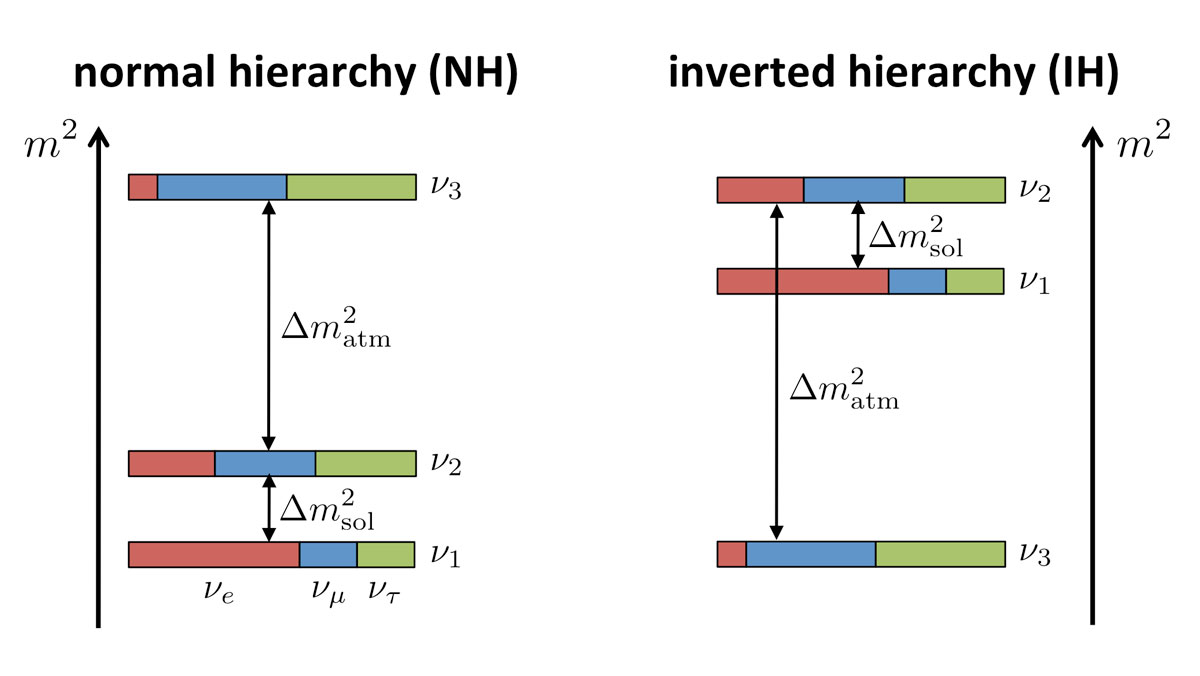
\includegraphics[width=0.8\textwidth]{mass-hierarchy.png}
 	\caption{\label{hierarchy:fig}Neutrino mass eigenstates possible orderings in normal (left) and inverted (right) hierarchy. The flavour composition of the three states is shown by dividing the bars into colors: red for $\nu_e$ blue for $\nu_\mu$ and green for $\nu_\tau$ . \cite{Giunti}}
 \end{figure}
 Concerning neutrino mass eigenvalues two scenarios are possible:  the so-called $normal$ and $inverted$ $ordering$. In
normal ordering, neutrino mass eigenvalues are ordered $m_1<m_2<m_3$, while in inverted
ordering $m_3<m_1<m_2$ (Fig. \ref{hierarchy:fig}). 


\subsection{Charge-parity symmetry violation}
Since all mixing angles are not null, if the Dirac phase $\delta$ is different from 0 or $\pi$, neutrino oscillations are CP violating phenomena. CP violation is manifested if the oscillation probability of $\nu_\alpha \rightarrow \nu_\beta$ are different from the CP conjugate $\bar{\nu}_\alpha \rightarrow \bar{\nu}_\beta$. An observable for such effects would then be the CP asymmetry:
\begin{equation}
\mathcal{A}_{\alpha\beta}^{CP}=P(\nu_\alpha \rightarrow \nu_\beta) - P(\bar{\nu}_\alpha \rightarrow \bar{\nu}_\beta); \ \ \ \ \alpha\neq\beta \ \text{and} \ \alpha,\beta=e,\nu,\tau
\end{equation}
In the three neutrino mixing case the magnitude of the CP violation is determined by the so-called Jarlskog invariant $J^{CP}$ in direct analogy with the quark sector:
\begin{equation}
\begin{split}
\mathcal{A}_{\alpha\beta}^{CP}=-16J^{CP}\sin\bigg(\frac{\Delta m_{12}^2}{4E}L\bigg) \sin\bigg(\frac{\Delta m_{23}^2}{4E}L\bigg) \sin\bigg(\frac{\Delta m_{13}^2}{4E}L\bigg) \\[10pt]
\text{with} \ J^{CP}= Im[U_{\alpha1}U_{\alpha2}^*U_{\beta1}^*U_{\beta2}]=\pm c_{12}s_{12}c_{23}s_{23}c_{13}^2s_{13}\sin\delta
\end{split}
\end{equation}
Current constraints for the mixing angles imply that the value of $J^{CP}$ should be in the range:
\begin{equation}
0.026|\sin \delta|\lessapprox |J^{CP}| \lessapprox 0.036 |\sin \delta|
\end{equation} 
The asymmetry observable can be approximated in the three-flavour case as \cite{deltaCP}:
 \begin{equation}
 \label{eq:asymmetry}
 \mathcal{A}_{CP} \simeq \frac{\cos\theta_{23} \sin2\theta_{12}}{\sin\theta_{23}\sin\theta_{13}}\bigg( \frac{\Delta m_{21}^2 L}{4E_\nu}\bigg)\sin\delta_{CP} + \text{matter effects}
 \end{equation}
\subsection{Two flavor scenario} 
\begin{figure}
	\centering
	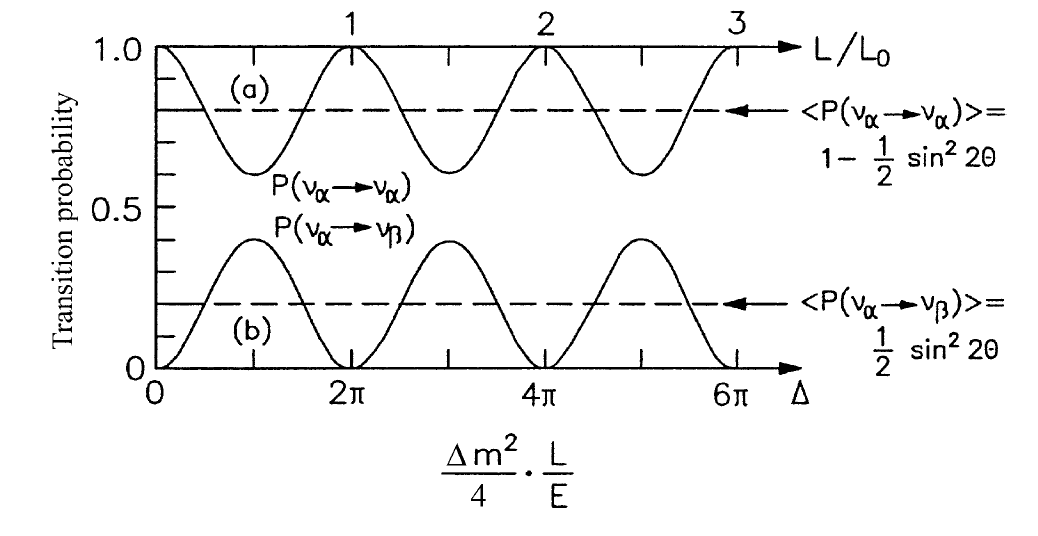
\includegraphics[width=0.55\textwidth]{2flavor_oscillation.png}
	\caption{\label{2oscillation:fig} Two flavour oscillation probability as a function of $L/L_0$, where $L_0=4E/\Delta m^2$: disappearance $P(\nu_\alpha\rightarrow \nu_\alpha)$ (upper curve); appearance $P(\nu_\alpha\rightarrow \nu_\beta)$ (bottom curve). \cite{Zuber} }
\end{figure}  
Since most experiments are sensitive to oscillations that are driven by a single squared mass difference, an important approximation of the neutrino oscillation phenomenon is the special case in which only two flavours are considered.\\
In this simplified case the mixing matrix is two dimensional and depends only on one mixing angle. In the case of $\nu_e$ and $\nu_\mu$ we get:
\begin{equation}
\begin{pmatrix}
\nu_e \\ 
\nu_\mu
\end{pmatrix}
=
\begin{pmatrix}
\cos\theta & \sin\theta \\ 
-\sin\theta & \cos\theta
\end{pmatrix}
\begin{pmatrix}
\nu_1 \\ 
\nu_2
\end{pmatrix}
\end{equation}
The two-flavour transition probability ,using the formulas from the previous section then becomes:
\begin{equation}
P(\nu_e\rightarrow \nu_\mu) = \sin^22\theta \sin^2\bigg( \frac{\Delta m^2L}{4E}\bigg)
\end{equation}
Since no CP symmetry violation is possible the probability is the same for $\nu_\mu\rightarrow \nu_e$ and for $\bar{\nu}_\mu\rightarrow \bar{\nu}_e$.\\
The $survival$ probability of the particle not changing flavour is simply:
\begin{equation}
P(\nu_e\rightarrow \nu_e)=1-P(\nu_e\rightarrow \nu_\mu)
\end{equation}
The oscillatory term can also be rewritten as:
\begin{equation}
\begin{split}
\sin^2\bigg( \frac{\Delta m^2L}{4E}\bigg)=\sin^2\bigg(\pi \frac{L}{L_0}\bigg) \\[8 pt]
\text{with} \ L_0=4\pi\frac{E}{\Delta m^2}
\end{split}
\end{equation}
where $L_0$ is the oscillation length and describes the period of one full oscillation cycle. It is proportional to $E$, and inversely proportional to $\Delta m^2$. The oscillation probability will then be maximum for $L/L_0=1/2$ and its amplitude will be given by $\sin^2\theta$ (Fig. \ref{2oscillation:fig}). 
\subsection{MSW matter effects}
\label{sec: matter effects}
When neutrinos travel through matter, they can coherently interact with electrons and nuclei in the medium and their oscillation probability is modified as it was first noticed by Mikhaev, Smirnov and Wolfenstein, from which the MSW effect takes its name \cite{Wolfenstein}. \\
The MSW effect has origin from the fact that $\nu_e$ are the only neutrino flavour that can take part both in charged current interactions, and NC elastic interactions with electrons, while $\nu_\mu$ and $\nu_\tau$ can only have NC interactions with electrons. This introduces an extra potential in the hamiltonian of the electron neutrinos:
\begin{equation}
V_e= \pm \sqrt{2} G_FN_e
\end{equation} 
where $N_e$ is the electron number density in the medium, $G_F$ is the Fermi constant and the sign is positive for neutrinos and negative for antineutrinos.\\
\begin{figure}
	\centering
	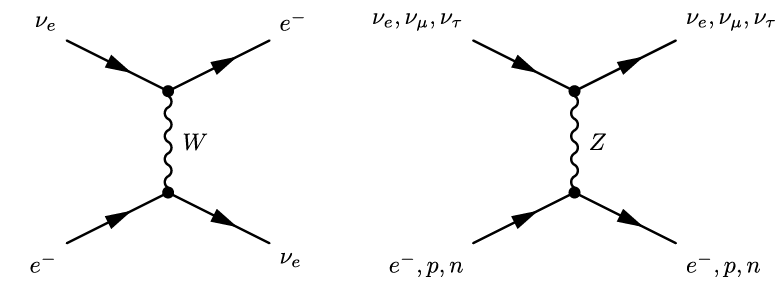
\includegraphics[width=0.8\textwidth]{WZ.png}
	\caption{\label{WZ:fig} Feynmann diagram of CC electronic neutrino interactions $\nu_e+e^- \rightarrow \nu_e+e^-$ (left) and of NC neutrino interactions $\nu_\alpha+e^- \rightarrow \nu_\alpha+e^-$ (right). }
\end{figure}
Using a simplified two flavour approach \cite{Ricciardi} the effective Hamiltonian of neutrino propagation in matter $\mathcal{H}_M$ then gains an extra $\nu_e-\nu_e$ element with respect to the Hamiltonian in vacuum $\mathcal{H}$ and becomes:
\begin{equation}
\mathcal{H}_M= 
\mathcal{H}+
\begin{pmatrix}
V_e & 0 \\
0 & 0
\end{pmatrix}
=
\bigg(\frac{\Delta m^2}{4E}\bigg)
\begin{pmatrix}
-\cos 2\theta & \sin 2\theta \\
\sin 2 \theta & \cos 2 \theta
\end{pmatrix}
+
\begin{pmatrix}
V_e & 0 \\
0 & 0
\end{pmatrix}
\end{equation}
In the simple case where the matter density is constant, we can then re-diagonalise $\mathcal{H}_M$ to obtain a new mixing matrix and mass eigenstates. We can then denote the new effective parameters as $\theta_M$ and $\Delta m_M^2$ and the oscillation probability takes the usual form:
\begin{equation}
P(\nu_e \rightarrow \nu_\mu)= \sin ^2 2 \theta_M \sin ^2 \bigg(\frac{\Delta m_M^2L}{4E}\bigg)
\end{equation}
The new parameters then become:
\begin{equation}
\begin{split}
&\Delta m^2_M =M\Delta m^2\\[8 pt]
&\sin 2\theta_m =\frac{\sin 2\theta}{M}
\end{split}
\end{equation}
with coefficient $M$ being:
\begin{equation}
M=\sqrt{\bigg(\cos 2\theta - \hat{A}\bigg)^2 + \sin^2 2 \theta}
\end{equation}
and:
\begin{equation}
\hat{A}=\pm \frac{2 \sqrt{2}G_FN_eE}{\Delta m^2}
\end{equation}
Matter effects have some very crucial consequences in the field of neutrino oscillation:
\begin{itemize}
	\item Oscillation probabilities can be different for neutrinos and antineutrinos even if there is no CP violation, due to the $\pm$ sign in the effective potential $V_e$.
	\item There is a resonant condition for which the oscillation probability is significantly enhanced with respect to the one in vacuum. That is when:
	\begin{equation}
	\hat{A} = \cos 2\theta
	\end{equation} 
	The resonant condition can be met only if $\hat{A} > 0$, which depends on the sign of the squared mass difference $\Delta m^2$. This fact makes matter effects an effective probe to study mass ordering. In particular it can be studied in long baseline accelerator experiments which are sensitive to muon-electron neutrino oscillation.
\end{itemize}
Note that either long travel distances or high matter densities are necessary in order for the MSW effects to be appreciable. If $\Delta m_M^2L/4E \ll 1$ we return to vacuum probabilities.
\clearpage
\section{Neutrino oscillation experiments}
\label{sec: Oscillation experiments}
The first subdivision between different neutrino oscillation experiments is determined by what the experiment is trying to measure \cite{Giunti}:
\begin{itemize}
	\item \textbf{Appearance experiments}: These experiments look for signals from neutrino flavours that are not present in the initial composition of the flux.
	\item \textbf{Disappearance experiments}: These experiments measure the number of signals from the various flavours of neutrinos and confront it with the expected one in order to compute the survival probability.
\end{itemize}
The second distinction is between the different sources of neutrinos. The most important ones are:
\begin{itemize}
	\item \textbf{Reactor experiments}: they use large fluxes of $\bar{\nu}_e$ produced by beta decays of fission fragments in nuclear power plants; 
	\item \textbf{Accelerator experiments}: they use beams of neutrinos produced in decays of secondary mesons (mainly $\pi$ and $K$), generated by a proton beam hitting a target;
	\item \textbf{Atmospheric neutrino experiments}: they detect neutrinos produced in the decays of mesons originated from the interactions of cosmic rays with nuclei in the atmosphere;
	\item \textbf{Solar neutrino experiments}: they detect neutrinos generated in thermonuclear reactions in the core of the Sun;
\end{itemize}
This distinction is important not only because of the very different experimental setups, but also because the neutrino source and where the detectors are located with respect to it, determine the constants of nature to which the experiments are sensitive. Specifically experiments can be sorted according to  the value of $\Delta m^2$ to which they are sensitive. The condition for an experiment to be sensitive to a specific mass squared difference is that:
\begin{equation}
\frac{\Delta m^2L}{2E}\sim 1
\end{equation}
If this value is too small the oscillation simply does not occur, if it is too large only the average transition probability is measurable and no information on $\Delta m^2$ can be obtained. The different experiments are then classified depending on the ratio $L/E$, which determines the sensitivity:
\begin{itemize}
	\item \textbf{Short Base-Line (SBL)}: These are either reactor or accelerator experiments. In the first case the experiments measure the survival probability and and are active in the $L/E$ range:
	\begin{equation}
	\frac{L}{E}\lesssim 10 \text{m/MeV} \ \ \Longrightarrow \ \ \Delta m^2 \gtrsim 1\text{eV}^2
	\end{equation}
		\item \textbf{Long Base-Line (LBN)}: these experiments have sources similar to SBL ones but have a distance between source and detector that is 10 or 100 times larger:
	\begin{equation}
	\begin{split}
	&\frac{L}{E}\lesssim 10^3 \text{km/GeV} \ \ \ \ \  \Longrightarrow \ \ \Delta m^2 \gtrsim 1\text{eV}^2 \ (Accelerator)\\ 
	&\frac{L}{E}\lesssim 10^3 \text{m/MeV} \ \ \ \ \ \  \Longrightarrow \ \ \Delta m^2 \gtrsim 1\text{eV}^2  \ (Reactor)\\
	\end{split}
	\end{equation}
	In this cathegory are also included the Atmospheric neutrino experiments:
	\begin{equation}
	\frac{L}{E}\lesssim 10^4 \text{km/GeV} \ \ \ \ \ \  \Longrightarrow \ \ \Delta m^2 \gtrsim 1\text{eV}^2  \ (ATM)
	\end{equation}
	
	\item \textbf{Very Long Base-Line (VLB)}: these experiments have a distance between source and detector that is 10 or 100 times larger then for  LBN experiments:
	\begin{equation}
	\begin{split}
	&\frac{L}{E}\lesssim 10^5 \text{m/MeV} \ \ \ \ \  \Longrightarrow \ \ \Delta m^2 \gtrsim 10^{-5}\text{eV}^2 \ (Reactor)\\ 
	&\frac{L}{E}\lesssim 10^4 \text{km/GeV} \ \ \ \ \ \  \Longrightarrow \ \ \Delta m^2 \gtrsim 10^{-4}\text{eV}^2  \ (Accelerator)\\
	\end{split}
	\end{equation}
	In this cathegory are also included the Solar neutrino experiments:
	\begin{equation}
	\frac{L}{E}\lesssim 10^{12} \text{m/MeV} \ \ \ \ \ \  \Longrightarrow \ \ \Delta m^2 \gtrsim 10^{-12}\text{eV}^2  \ (Sol)
	\end{equation}
	
\end{itemize}

\subsection{Solar experiments: $\theta_{12}$ and $\Delta m_{12}^2$}
\label{sec: Solar experiments}
\begin{figure}
	\centering
	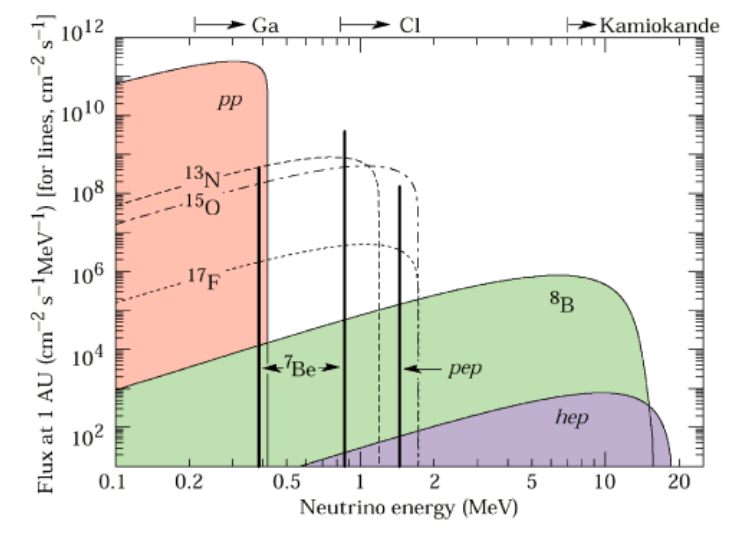
\includegraphics[width=0.7\textwidth]{SSM.png}
	\caption{\label{SSM:fig} Spectrum of solar neutrinos, modelled from the SSM. The arrows indicate the sensitivity range of some of the experiments. \cite{Bahcall} }
\end{figure}
The Sun produces an intense flux of neutrinos as a sub-product of some of the thermonuclear reactions that produce energy in its interior by burning hydrogen into helium \cite{Bahcall}. There are two main cycles of  reactions that can produce neutrinos: the pp (proton-proton) cycle and CNO (Carbon-Nitrogen-Oxygen) cycle. Both can be summarized as:
\begin{equation}
4p \rightarrow \ ^4He+2 e^- + 2\nu_e
\end{equation}  
The expected flux of $\nu_e$, can be computed using the standard solar model (SSM), which is a detailed mathematical model of the reactions taking place in the solar interior (Fig. \ref{SSM:fig}).\\
The solar neutrino experiments can be divided into two main categories depending on the revelation techniques: radiochemical and Cherenkov. In the first field we find experiments such as Homestake, Gallex/GNO and Sage \cite{Homestake} \cite{Gallex} \cite{Sage}. These experiments exploit the Inverse Beta Decay (IBD) reaction of solar neutrino with $^{37}$Cl, $^{71}$Ga and $^{71}$Ge respectively). These have a relatively low energy threshold ($E_\nu\gtrsim 0.23-0.81$ MeV), but they are not able to give any information on  direction, energy or time of the event.\\
The Cherenkov technique was pioneered by the Kamiokande experiment \cite{SuperK}, consisting of a tank of about 3000 tons of pure water and 1000 photomultipliers positioned on the inner walls. The experiment observed the Cherenkov light produced by recoil electrons in  elastic scattering interactions of $\nu_e$ with $e^-$, which have an energy threshold of $E\gtrsim 5 \text{MeV}$:
\begin{equation}
\text{(ES)} \ \ \nu_e + e^- \rightarrow \nu_e + e^- \ \ \ \ E\gtrsim 5 \text{MeV}
\end{equation}
\begin{figure}[t]
	\centering
	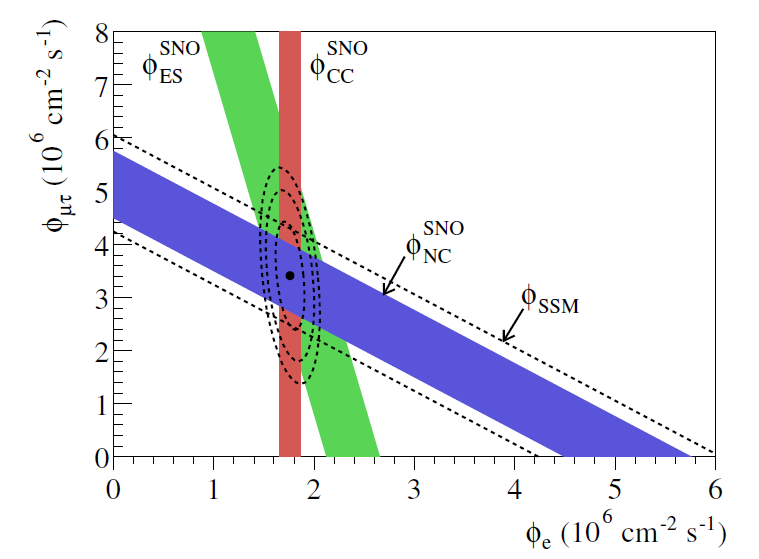
\includegraphics[width=0.7\textwidth]{SNO.png}
	\caption{\label{SNO:fig} Flux of muon and tau neutrinos $\phi_{\mu\tau}$ over electron neutrino $\phi_e$ as measured by SNO. The three coloured bands correspond to the three possible interactions: electron scattering ES (green); charged current CC (red); neutral current NC (blue). The dashed band gives the prediction from the SSM which is in agreement with the NC measurements. \cite{SNO}   }
\end{figure}
This technique was capable of measuring neutrino interactions in real time while also giving informations on direction and energy. This capability was crucial in confirming the existence of the so called \textit{solar neutrino problem}, a deficit in the number of neutrinos arriving from the Sun between 1/2 and 2/3 with respects to the predictions of the SSM, measured by the earlier radiochemical experiments. \\
The Kamiokande experiment was able to measure only the flux of $\nu_e$. Differently, the SNO experiment, thanks to the use of heavy water ($d_2O$) rather than purified water as target, had access to two more reactions for detection \cite{SNO}:
\begin{equation}
\begin{split}
\text{(CC)} & \ \ \ \nu_e+d \rightarrow p+p+e^-; \ \ \ E\gtrsim\text{5MeV} \\
\text{(NC)} & \ \ \ \nu_f+d \rightarrow p+n+\nu_f; \ \  f=e,\mu,\tau  \ \ E\gtrsim\text{2.2MeV}
\end{split}
\end{equation}  
With the first reaction being sensitive only to $\nu_e$ and the second being sensitive to all flavours. What SNO found was that the combined tau and mu fluxes were two
times more intense than the $\nu_e$ one and that the total flux was in agreement with the predictions from the SSM (Fig. \ref{SNO:fig}). \\
The characteristic L/E for the solar experiments are of the VLB range, making them sensitive to the $\Delta m^2_{12}$ squared mass difference and to $\sin2\theta_{12}$. For this reason the two parameters are often referred to as solar mass difference and solar mixing angle ($\Delta m^2_\odot, \theta_\odot$). As already noted these two parameters can be measured also by VLB reactor experiments such as KamLand \cite{kamland}. The most precise values for the parameters are obtained combining the results from both (Figure \ref{kamland:fig}).\\
Other important and more recent Solar experiments include Borexino \cite{Borexino}, which was the first with an energy threshold low enough to measure the monochromatic flux of $^7Be$ and $pep$ neutrinos and Super-K, the successor of Kamiokande. The results from both experiments are in agreement with the neutrino oscillation hypothesis.

\subsection{Reactor experiments}
\label{sec: Reactor experiments}
\subsubsection{VLB: confermation of solar experiment results}

\begin{figure}
	\centering
	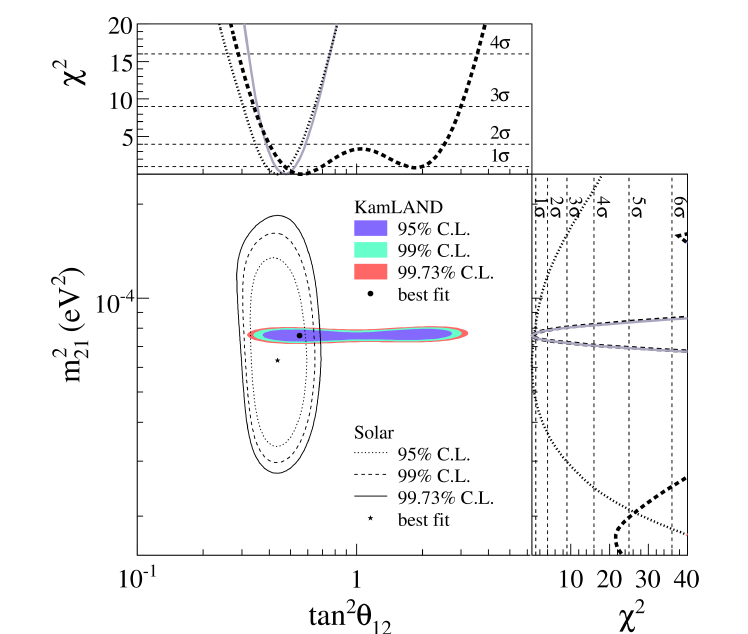
\includegraphics[width=0.7\textwidth]{kamland.png}
	\caption{\label{kamland:fig} Confidence level intervals for the solar oscillation parameters from KamLAND and the combined results from solar experiments. The side-panels show the respective $\chi^2$ profiles: KamLAND (dashed); solar experiments individually (dotted); combined (solid). \cite{kamland}}
\end{figure}
Neutrinos from nuclear reactors are $\bar{\nu}_e$ with energy of the order of the MeV. This makes the particles above threshold for electronic CC interactions, but not for other flavours, which means that if the neutrino oscillates CC interactions cannot happen. Reactor experiments can then measure the disappearance probability of the $\bar{\nu}_e$ and they are usually sensitive to small values of $\Delta m^2$ due to the low energy spectrum of the neutrinos. \\
Very Long Baseline experiments proved to be sensitive to the solar square mass difference and were able to give confirmation on the Solar experiment results, while at the same time improving the sensitivity to the parameter and beginning the precision era of neutrino physics. \\
In particular the KamLAND experiment, located in the Kamioka mines in Japan , was the first to give independent confirmation of the results from the solar neutrino sector. It consists of a 1000 ton liquid scintillator detector measuring the interactions of $\bar{\nu}_e$ from a cluster of nuclear reactors located  at an average distance of $L \simeq 175$ km. The antineutrinos interact via inverse beta decay at an energy threshold of $E>2.6$ MeV:
\begin{equation}
\bar{\nu}_e + p \rightarrow e^+ +n \ \ \ \ E>\text{2.7 MeV}
\end{equation}
The experiment exploited the signature given by the $e^+$ annihilation and the delayed neutron thermalisation and capture proved very effective in the reduction of background. This level of precision was also crucial in excluding alternative explanations for neutrino oscillations based on exotic interactions or magnetic transition moments \cite{Wagner}.

\subsubsection{Measurement of $\theta_{13}$ }
\begin{figure}
	\centering
	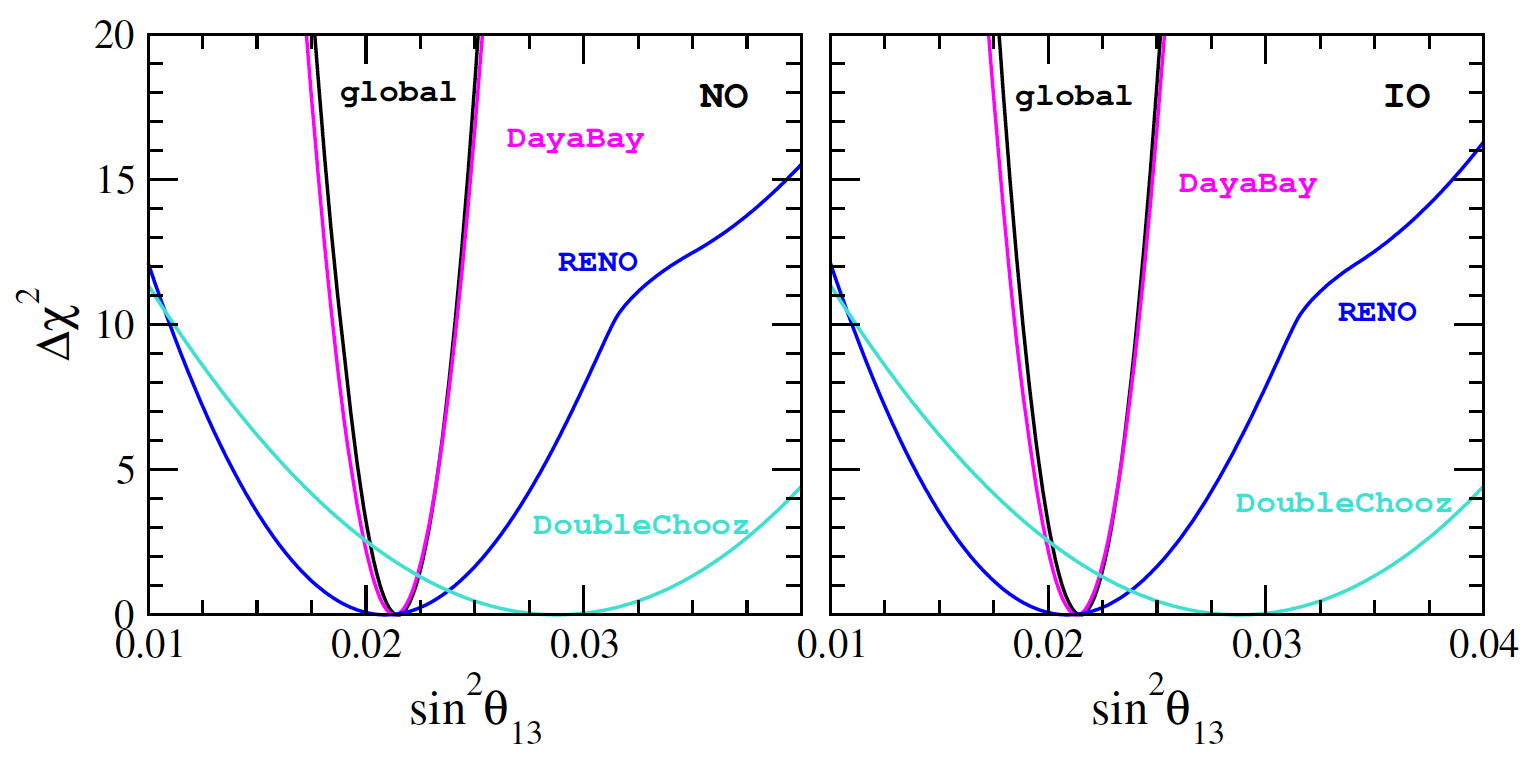
\includegraphics[width=0.8\textwidth]{theta13.png}
	\caption{\label{theta13:fig} $\chi^2$ profile as a function of $\sin\theta_{13}$ for RENO DataBay and Double Chooz and the combined result (black line). The results are fitted for normal ordering (left) and inverse ordering (right). \cite{Farzan-Tortola}}
\end{figure}
Recently Short Baseline experiments such as Data Bay \cite{Data Bay}, RENO \cite{RENO} and Double Chooz \cite{Double Chooz} have been able to measure the disappearance of reactor electron antineutrinos at distances $L\sim$1 km. Their characteristics made them sensitive to the measurement of the $\theta_{13}$ mixing angle.\\
Compared to previous experiments such as CHOOZ and Paloverde,  these have not only access to larger statistics, thanks to the increased reactor power and larger detectors, but they also have access to multiple detectors at different distances from the reactor core. Measurements at the closest detectors can then be utilized to more accurately predict the expected number of events at the more distant ones. The combined results from the experiments are shown in Figure \ref{theta13:fig}
\subsection{Atmospheric experiments: $\Delta m_{31}^2 $ and $ \theta_{23}$}
\label{sec: atmospheric experiments}
\begin{figure}
	\centering
	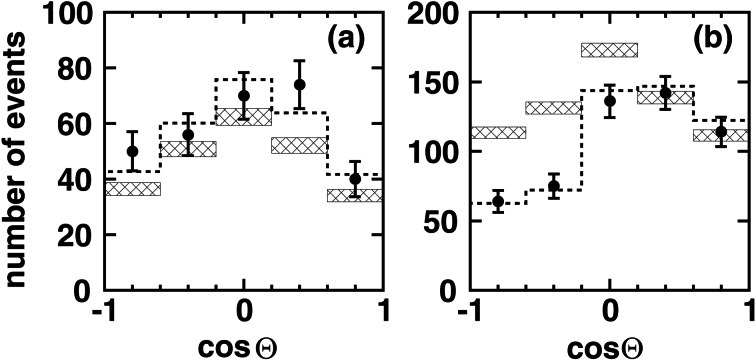
\includegraphics[width=0.9\textwidth]{superk.png}
	\caption{\label{superk:fig} Zenith angle $\Theta $ distributions for the most energetic multi-GeV atmospheric neutrino events measured by Super-Kamiokande over a 535 days period. Filled histograms are the Monte Carlo predictions and dotted histograms are the experimental measurements. Right and left panels are $\mu$-like and e-like events respectively. \cite{Superk atm}}
\end{figure}
\begin{figure}
	\centering
	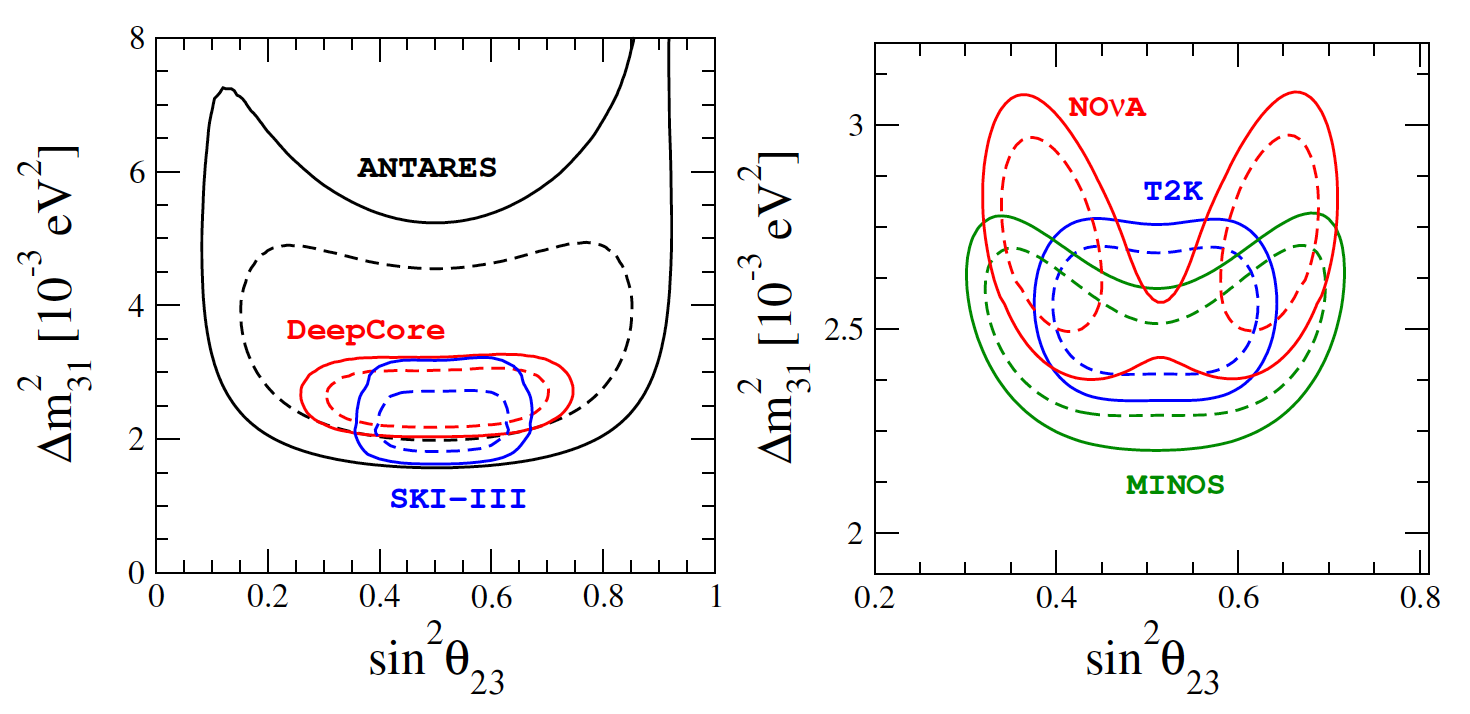
\includegraphics[width=0.9\textwidth]{atmnu.png}
	\caption{\label{atmnu:fig}90\% CL (straight line) and 99\% C.L.(dashed line) regions in the atmospheric parameter plane ($\Delta m_{31}^2$ over $\sin^2 \theta_{23}$ from atmospheric (left) and long baseline accelerator (right) experiments, assuming normal mass hierarchy. \cite{Farzan-Tortola} }
\end{figure}
The cosmic ray interactions with the atmosphere nitrogen and oxygen nuclei produce mostly pion and kaons that decay in electron and muon neutrino as well as antineutrinos. $\nu_e$ decay from the chain : $\pi \rightarrow \mu \nu_\mu$ followed by $\mu \rightarrow e \nu_\mu \nu_e $ . One then would expect the ratio to be of the order:
 \begin{equation}
 R= \frac {N (\nu_\mu + \bar{\nu}_\mu)}{N (\nu_e + \bar{\nu}_e )} \sim 2
 \end{equation}
Experiments originally built to look for proton decay in the '70s and '80s, which had atmospheric neutrinos as background, were the first to observe a deficit of the muon neutrino flux with respect to the Monte Carlo expectations, measured originally as the ratio : $R_{\mu / e}/ R_{\mu/e}^{MC}$. Two main categories of detectors were in operation: water Cherenkov tanks such as Super Kamiokande \cite{Superk atm} and iron calorimeters such as Soudan2 \cite{soudan 2} and Macro \cite{MACRO}. The first kind of detectors are constituted of tanks filled with water of the order of 1 ton, and they detect the Cherenkov light rings produced by the charged lepton produced in the neutrino CC interaction using photo multipliers placed on the inside of the walls. Iron calorimeters are instead constituted of layers of iron, acting as a passive materials and active layers, made for example of plastic scintillators, which track either the electromagnetic showers produced by $e^\pm$ or long muon tracks. Both techniques are capable of flavour identification and direction and energy estimation.\\
In 1998 the Super-Kamiokande was among the first to observe an anomalous deficit. The experiment distinguished between muon and electron neutrino events, measured the lepton zenith angle with respect to the Earth's axis (correlated to that of the parent neutrino direction) and divided the samples differentiating according to the lepton energy (the more energetic events having a stronger direction dependency with that of the parent neutrino). These measurements made it possible to observe the variation of the flux as a function of the energy and zenith angle and thus the $L/E$ travelled by the parent neutrino (Figure \ref{superk:fig}).\\
 Super-Kamiokande showed that while the electron events had no reduction, the muon events had a deficit of almost 50\% for up-going neutrinos ($\cos\Theta = -1$). The results can be explained considering as due to the neutrino oscillation phenomena driven by the parameters $\Delta m_{23}^2$ and $\theta_{23}$ that for this reason are often referred to as atmospheric oscillation parameters : $\Delta m_{ATM}^2, \ \theta_{ATM}$. The best fit values for these parameters are today given by combining the results of Super-Kamiokande with the ones from modern neutrino telescopes ANTARES and IceCube (Figure \ref{atmnu:fig}). 
\subsection{Accelerator experiments}
\label{sec: accelerator experiments}
\begin{figure}[t!]
	\centering
	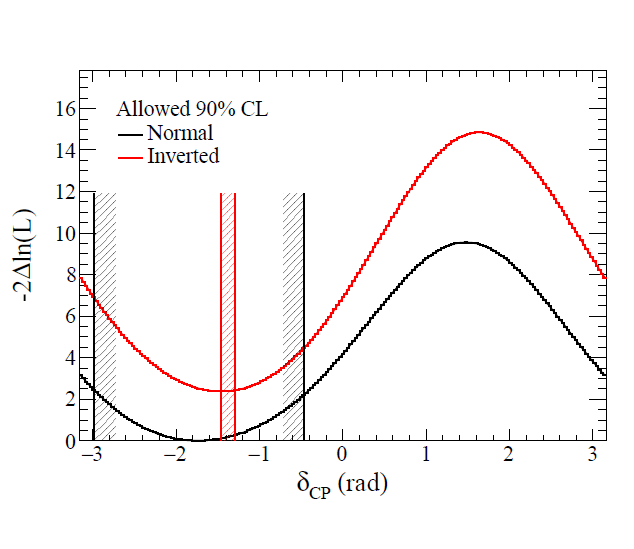
\includegraphics[width=0.48\textwidth]{cpt2k.png}
	\hfill
	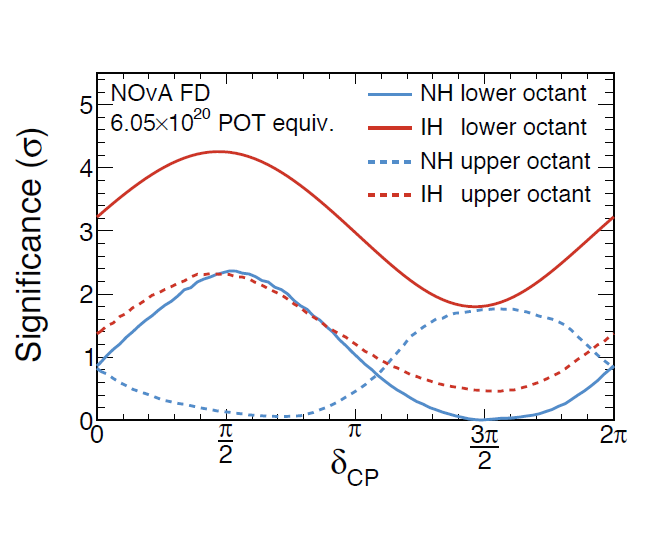
\includegraphics[width=0.48\textwidth]{cpnova.png}
	\caption{\label{cp:fig} (Left) Log-likelihood function of $\delta_{CP}$ with 90\% CL for normal (black) and inverted (red) hyerarchy at T2K (Right) Significance as function of $\delta_{CP}$ at NO$\nu$A in all combinations of mass ordering and $\theta_{23}$ octant. \cite{t2k deltacp} }
\end{figure}
The first two experiments to confirm the atmospheric oscillation results were K2K (KEK to Kamioka) in Japan and MINOS at Fermilab. K2K used a beam of about 98\% $\nu_\mu$ with a mean energy of about 1.3 GeV produced from 12 GeV protons accelerated at the KEK synchrotron. The experiment had a near detector at about 300 m from the proton target, and used Super-Kamiokande as its far detector at about 250 km. The K2K data sample taken from 1999 to 2005 (K2K-I and II) contained about 112 muonic events versus the 158 expected without oscillation, confirming the findings in the atmospheric sector \cite{k2k}. MINOS also looked for $\nu_\mu$ disappearance using the NuMi neutrino beam at $E\sim3$GeV. Much like K2K it had a near detector at about 1 km from the source and a second detector in the Soudan mines at about 735 km away as its far detector. The first results published in 2006, combined with the ones from K2K first confirmed neutrino oscillations at 5$\sigma$ \cite{MINOS}.\\
Long Baseline experiments such as OPERA and ICARUS worked instead in the appearance channel looking for signatures of $\nu_\tau$ in $\nu_\mu$ beams. The OPERA experiment in particular found 5 $\nu_\tau$ candidates in a sample of $1.8 \times 10^{19}$ POT (protons on target) from the CNGS beam. This was enough to confirm muon neutrino oscillation at 5$\sigma$ \cite{OPERA}. Short baseline experiments such as NOMAD \cite{Nomad} and CHORUS \cite{Chorus} at CERN also studied the $\nu_\mu \rightarrow \nu_\tau$ channels but did not observe any oscillations. \\
Current experiments such as T2K  (Tokai to Kamioka) \cite{T2K}, the successor of K2K, and NoVA\cite{Nova} both use muon neutrino beam and perform precision measurements in both appearance and disappearance channels. Allowed CL areas for the atmospheric parameters $\Delta m_{31}^2$ and $\sin^2 \theta_{23}$ obtained from T2K, NoVa and MINOS data can are shown in Figure \ref{atmnu:fig}.
\subsection{$\delta_{CP}$ experimental results}
The latest measurements of $\delta_{CP}$ are from T2K \cite{t2k deltacp}. The experiment measured both the $\nu_\mu$ survival probability and the $\nu_e$ appearance probability and then did the same for $\bar{\nu}_\mu$. The analysis excludes $\delta_{CP}=0^\circ,\pm 180 ^\circ$ at 90\% CL for both mass orderings.\\
Similar measurements have been performed by the NO$\nu$A experiment. The analysis found two best-fit points for normal mass ordering : $\sin^2\theta_{23}= 0.404$ $\delta_{CP}=1.48\pi$ and $\sin^2\theta_{23}= 0.623$ $\delta_{CP}=0.74\pi$. It also found that the inverted mass ordering is disfavoured at $>93\%$ regardless of the value of the CP phase.
\begin{figure}
	\centering
	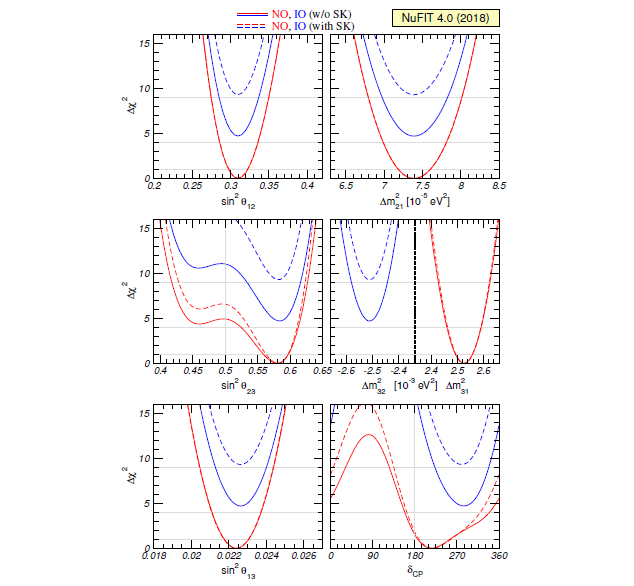
\includegraphics[width=0.7\textwidth]{massexp.png}
	\caption{\label{masshierarchy3:fig} $\Delta\chi^2$ profile obtained from global 3$\nu$ oscillation experiments analysis. The profiles are minimized in all non displayed parameters. The red and and blue full curves correspond to the analysis results for NO and IO respectively, without considering the atmospheric data from SuperK. The dashed lines are with the inclusion of this data. For atmospheric mass squared difference $\Delta m_{31}^2$ is used for NO and $\Delta m_{32}^2$ for IO. \cite{mass global fit}}
\end{figure}
\subsection {Mass hierarchy experimental results}
The most recent global fits performed on the oscillation parameters $\Delta m_{32}^2$, $ \Delta m_{31}^2$, $ \delta_{CP}$ and $\sin^2\theta_{23}$ from LBL accelerator experiments (NO$\nu$A, MINOS, T2K), reactor experiments (Data Bay, RENO, Double Chooz) and solar experiments (SNO, SuperK, Borexino) show a growing preference towards standard hierarchy. In particular NO is preferred to IO with $\Delta\chi ^2=4.7$ (Figure \ref{masshierarchy3:fig}). The indication becomes even stronger when one includes data from the measurements on atmospheric neutrinos for Super-Kamiokande where NO is preferred with $\Delta\chi^2 = 9.3$ \cite{mass global fit}.
\section{State of the art and future prospects}
\begin{figure}
	\centering
	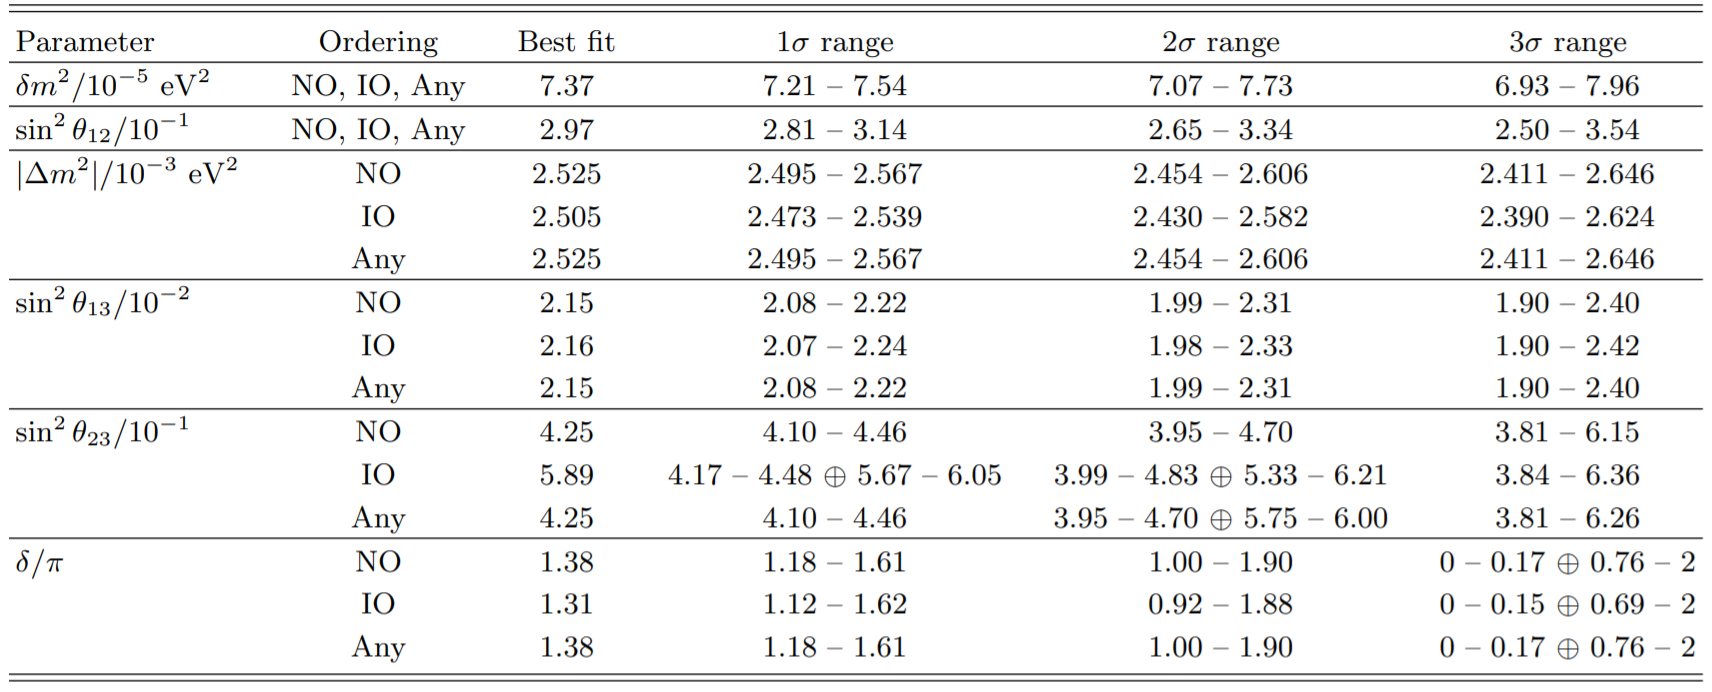
\includegraphics[width=1\textwidth]{stateoftheart.png}
	\caption{\label{stateof the art:fig} Results of recent $3\nu$ oscillation parameters global fits. The results are given in terms of best fit and $n\sigma$ ranges under the IO, NO and any ordering assumptions. Note that here $\delta m^2 \equiv \Delta m_{12}^2$, $\Delta m^2 = m_3^2-(m_1^2+m_2^2)/2$ and $\delta \equiv \delta_{CP}$ is given in terms of cycle intervals $\delta/\pi \in [0,2]$. \cite{global constraints}} 
\end{figure}
Neutrino physics is now entering its precision era, but nonetheless there are still fundamental questions that are yet to be fully answered : 
\begin{itemize}
	\item The determination of the absolute mass of the neutrinos and its origin i.e Majorana or Dirac;
	\item The measurement of CP asymmetries in the leptonic field;
	\item The determination of the mass ordering (normal or inverse)
\end{itemize}
While the first field of research is in the domain of the types of experiments described in Section \ref{sec: mass limits}, the latter two are best studied in oscillation experiments. Such goals will require levels of precision still not achieved and new experiments in all categories (reactor, atmospheric, ecc.). \\
In the long-baseline accelerator field DUNE (Deep Underground Neutrino Experiment), will be the next-generation flagship neutrino oscillation experiment of the Fermilab national laboratories. Having access to MSW effects and to a neutrino beam capable of producing both $\nu_\mu$ and $\bar{\nu}_\mu$ will make it particularly well suited to determine the mass ordering and observe CP violations. Precisely what constitutes DUNE and what are its experimental goals will be the subject of Chapter 2.


%%%%%%%%%%%%%%%%%%%%%%%%%%%%%%%%%%%%%%%%%%%%%%%%%%%%%%%%%%%%%%%%%%%%%%%%%%%%%

\chapter{DUNE}
\rhead[\fancyplain{}{\bfseries Chapter 2: DUNE}]{\fancyplain{}{\bfseries\thepage}}
\lhead[\fancyplain{}{\bfseries\thepage}]{\fancyplain{}{\bfseries Chapter 2: DUNE}}
          \label{chapter 2}
The Deep Underground Neutrino Experiment (DUNE) will be a new generation world-leading Long Baseline oscillation experiment. Among its main goals are the precise measurement of the oscillation parameters, the study of matter-antimatter asymmetry and the determination of the neutrino mass ordering. It is conceived around three main components: The neutrino beam facility, which is able to produce an intense and wide band muon neutrino and antineutrino beam; a Near Detector (ND) situated at the Fermi National Accelerator Laboratories (Fermilab, Batavia, Illinois); a multiple massive Liquid Argon Time Projection Chamber (LArTPC) Far Detector (FD) complex placed 1300 km downstream at the Sanford Underground Research Facility (Lead, South Dakota).\\
In this Chapter we will discuss DUNE's physics programme (Section 1) as well as the configuration of the neutrino beam and its main detectors (Section 2). The SAND detector, which is one of DUNE's Near Detectors system is the subject of the studies performed in this thesis and will be discussed more in detail in the next chapter.
\begin{figure}[t]
	\centering
	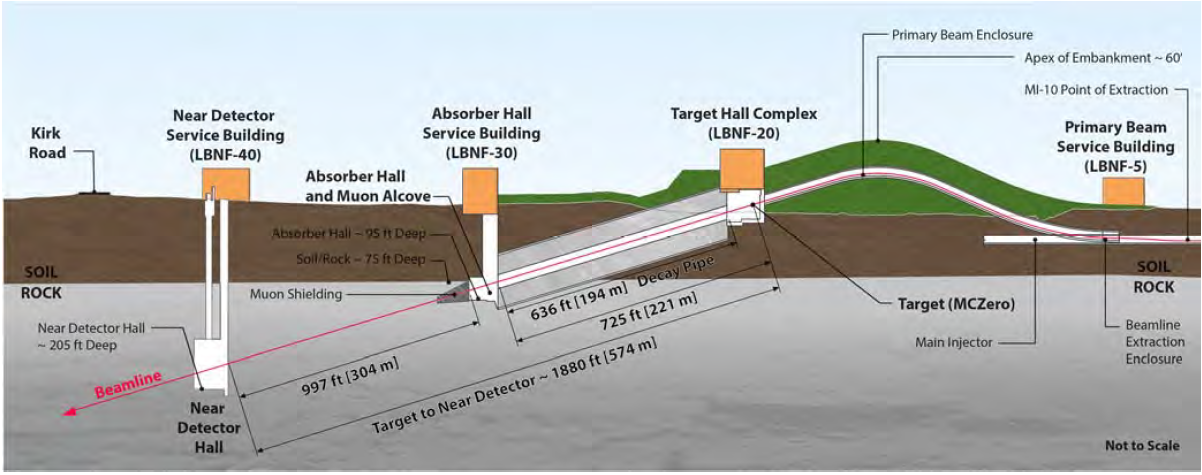
\includegraphics[width=\textwidth]{NeutrinoBeam.png}
	\caption{\label{NeutrinoBeam:fig} Schematic representation of the LBNF neutrino beamline facilities at Fermilab \cite{DUNE 3}. } 
\end{figure}
\section{LBNF/DUNE's facilities and design}
The experimental facilities and detectors will be divided between the Long-Baseline Neutrino Facility (LBNF), hosted by Fermilab and the DUNE collaboration. The first will provide the facilities in Illinois (Near Detector Facilities) and South Dakota at SURF (Far Detector facilities), necessary for the scientific program of DUNE. The collaboration will supervise the neutrino beam with the necessary upgrades, the ND conventional facilities in Fermilab and the construction of the caverns necessary to host the four liquid Argon far detectors. The DUNE collaboration will overview the design and construction of the detectors themselves \cite{DUNE 4}.
\subsection{LBNF beamline}
The LBNF BeamLine at Fermilab is a horn-focused, sign-selected neutrino beam, designed to meet the DUNE's long-baseline physics requirements \cite{DUNE 3}. It is focused towards the South Dakota facilities hosting the Far Detectors, 1480 m underground and 1300 km away from the FNAL facilities.\\
The main components of the beamline are shown in Figure \ref{NeutrinoBeam:fig}. A primary beam of accelerated protons (60-120 GeV) is produced in the Fermilab Main Injector (MI) (the primary beam main specifications and characteristics for 12 GeV protons are listed in Table \ref{tab:beam}). It is then extracted and transported through a man-made hill, at the apex of which it is bent downwards, toward a target at ground level, in the LBNF Target Hall. The total bend amounts to $7.2^\circ$ westward and $5.4^\circ$ downwards and directs the flux toward the Far Detectors.\\
When the accelerated protons hit the target, mesons are generated; these are then focused by magnetic horns into a decay pipe where they decay into muons and neutrinos.The decay pipe is 194 m long in total, with an additional 27 m acting as the target chase. The focusing structure, consisting of the two horns (placed 6.6 m apart and absorbing 230 kA ), provides neutrinos in the energy range 0.5-5 GeV, which is enough to cover the first two oscillation nodes (for a 1300 km baseline 2.4 and 0.8 GeV respectively).\\
\begin{figure}[t!]
	\centering
	\begin{subfigure}[b]{0.475\textwidth}
		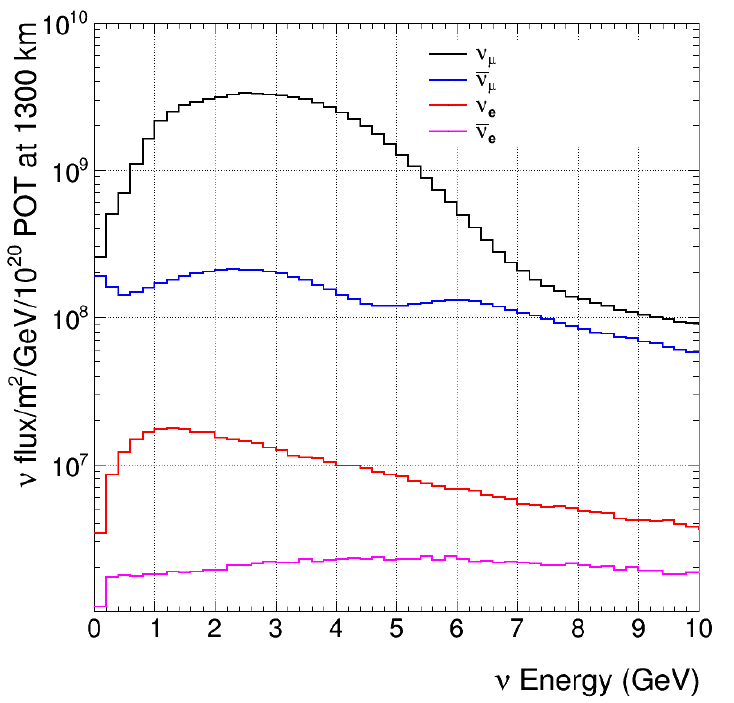
\includegraphics[width=\textwidth]{PosNu.png}
		\caption{}
	\end{subfigure}
	\hfill
	\begin{subfigure}[b]{0.475\textwidth}
		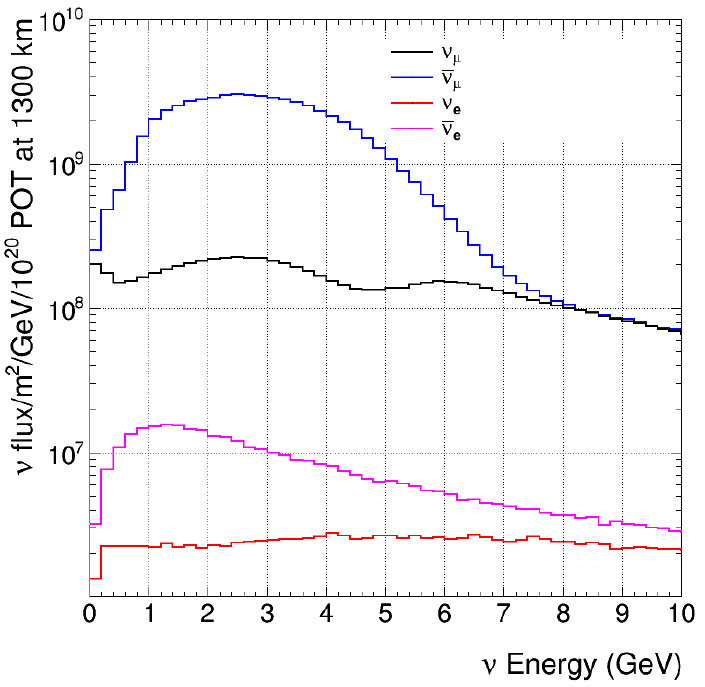
\includegraphics[width=\textwidth]{NegNu.png}
		\caption{}
	\end{subfigure}
	\caption{\label{NuSpectrum:fig} Expected neutrino and antineutrino beam produced focusing positive (a) and negative (b) mesons. \cite{DUNE 3}} 
\end{figure}
\begin{table}[b!]
	\centering
	\setlength{\tabcolsep}{8pt}
	\renewcommand{\arraystretch}{1.3}
	\begin{tabular}{ c c }
		\hline\hline
		Parameter & Value \\
		\hline
		Energy & 120 GeV \\
		Protons per cycle & $7.5\times10^{13}$ \\
		Spill duration & $1.0 \times 10^{-5}$s\\
		POT per year & $1.1\times10^{21}$ \\
		Cycle Time & 1.2 s \\
		Beam Power & 1.2MW \\
		Beam size at target & 1.5-1.7 mm \\
		$\Delta p / p$ & $11 \times 10^{-4}\ 99 \%\ (28\times10^{-4}\ 100 \%)$ \\
		Transverse emittance & 	$30\pi\ \mu m \ 99 \% \ (360 \pi \ \mu m\ 100 \%)$ \\
		Beam divergence (x,y) & 15-17 $\mu rad$ \\	
		\hline\hline
	\end{tabular}
	\caption{\label{tab:beam}Summary of the main primary proton beam parameters \cite{DUNE 3}}
\end{table}%
\clearpage
The horn polarity can be changed shifting between to current configurations: FHC (Forward Horn Current) and RHC (Reverse Horn Current). This makes it possible to selectively focus only positive or negative hadrons, thus producing either $\nu_\mu$ or $\bar{\nu}_\mu$ fluxes respectively. Both polarities will produce high purity fluxes, with an expected contamination from the ``incorrect" neutrino type (i.e. $\nu_\mu$ in RHC mode and vice-versa) of less than 10\% in the oscillation energy region. This type of impurities are introduced by hadrons of the opposite sign propagating at the centre of the beam, where no magnetic field is present. A small $\nu_e$ and $\bar{\nu}_e$ component is also introduced by the decay of secondary kaons and tertiary muons from pion decays. The neutrino and antineutrino expected fluxes obtained focusing  positive and negative particles are shown in Figure \ref{NuSpectrum:fig}. \\
The facility is set to run initially with a power of 1.2 MW (later upgrading to 2.4 MW), corresponding to $1.1 \times 10^{21}$ protons-on-target (POT) per year, for 120 GeV protons. This assumes that $7.5\times10^{13}$ protons are produced for each 1.2 s MI cycle and a total efficiency of 0.56 for the entire focusing and transportation system in LBNF.\\
\subsection{FD reference design: single phase LArTPC }
The reference design for DUNE's Far Detector consists of four 10 kt single-phase liquid Argon time projection chambers (for a total fiducial mass of 40 kt), each suspended inside a cryostat and augmented with a photon detection system (a model of the reference design is shown in Figure \ref{FD-SinglePhase:fig}). \\
The LArTPC technology has been pioneered by ICARUS. The charged particles in liquid Argon (LAr) produce ionization and scintillation light. The electrons drifting from production points towards the segmented anode plane producing a signal are then used to provide spatial information. The prompt scintillation photons are collected by a photon detection system that provide the absolute timing of the event. In particular a detector is single-phase if the ionization, drift and collection all occur in liquid Argon.\\
The two main active components of the detector are then the actual Time Projection Chamber (TPC) and the Photon Detection System (Photon Detector System), with the electronics divided in Cold Electronics (CE), mounted inside the Liquid Argon TPC, and the rest of the Data Aquisition System (DAQ).
\clearpage
\begin{figure}
	\centering
	\begin{subfigure}[b]{0.8\textwidth}
		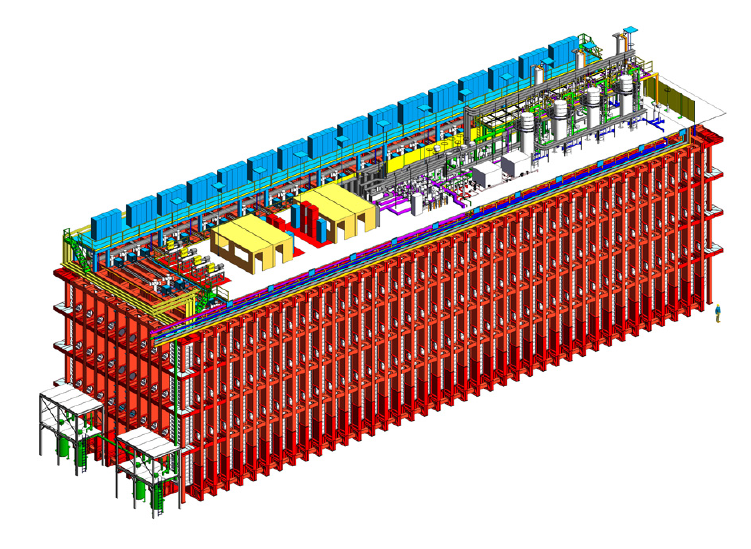
\includegraphics[width=\textwidth]{10kt.png}
		\caption{}
	\end{subfigure}
	\\
	\begin{subfigure}[b]{0.8\textwidth}
		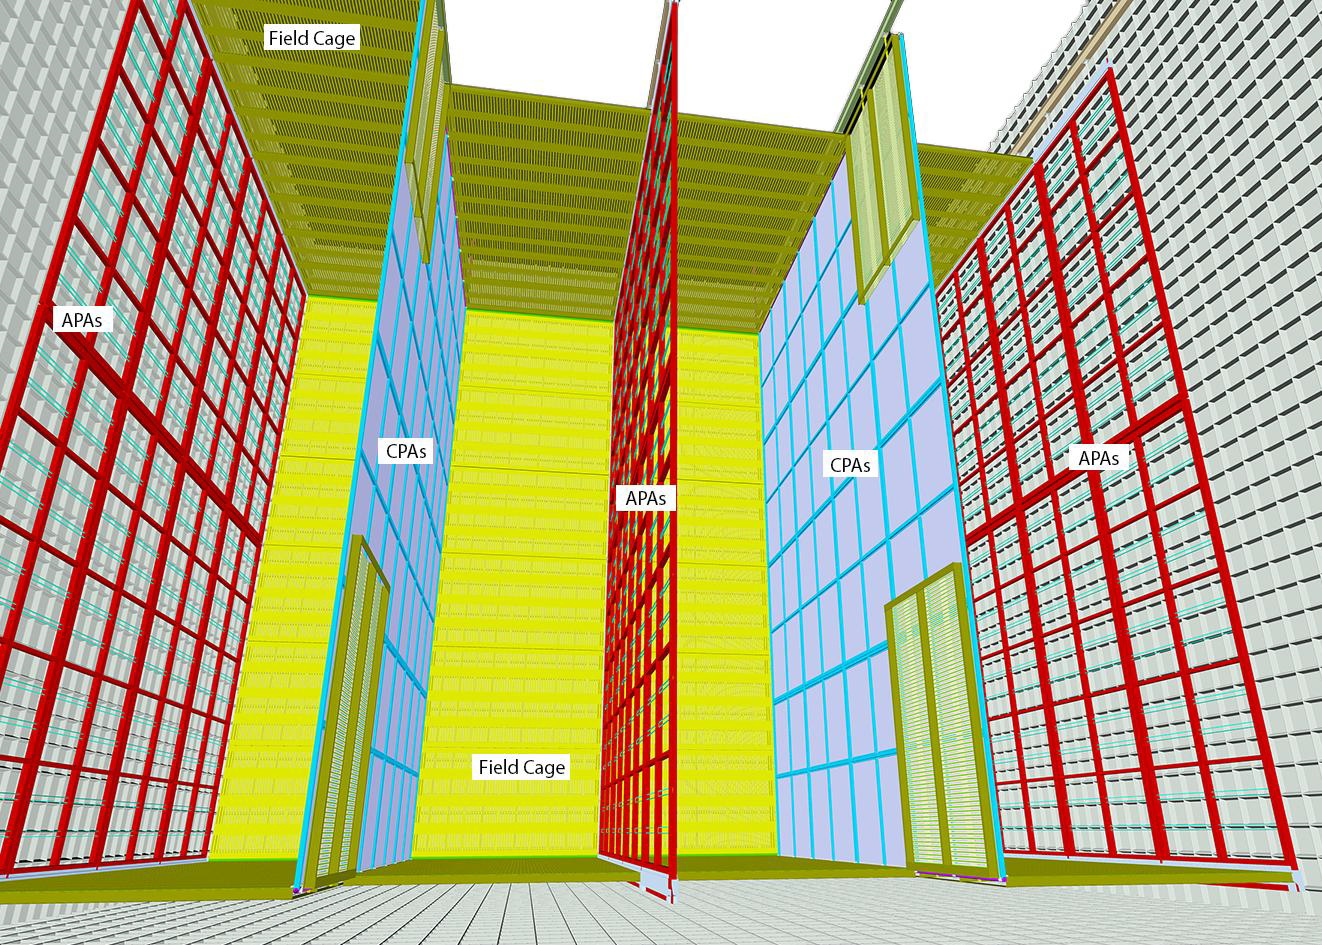
\includegraphics[width=\textwidth]{FD-SinglePhaseIn.png}
		\caption{}
	\end{subfigure}
	\caption{\label{FD-SinglePhase:fig} 3D Model of the FD single-phase reference design seen from outside (a) and inside of the TPC (b) \cite{DUNE 4}} 
\end{figure} 
\clearpage
\subsubsection{The time projection chamber (TPC)}
\begin{figure}[t!]
	\centering
	\begin{subfigure}[b]{0.23\textwidth}
		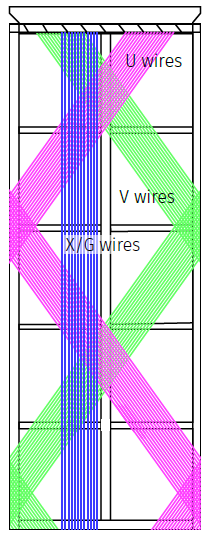
\includegraphics[width=\textwidth]{APA.png}
		\caption{}
	\end{subfigure}
	\hfill
	\begin{subfigure}[b]{0.7\textwidth}
		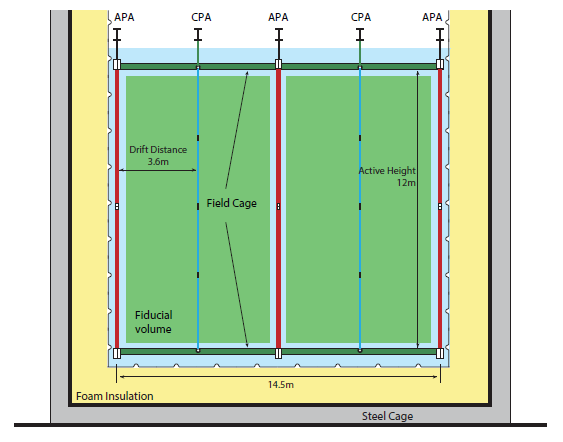
\includegraphics[width=\textwidth]{TPC-Slice.png}
		\caption{}
	\end{subfigure}
	\caption{\label{TPC:fig} (a) Wiring scheme of an APA module (b) Front schematic view of the inside of the TPC \cite{DUNE 4}} 
\end{figure} 
The TPC is the fundamental detector of DUNE's FD design. It is located inside an external cryostat keeping its temperature at 88 K (necessary to keep the Argon in its liquid phase) and is built modularly from by anode plane assemblies (APA), cathode plane assemblies (CPA) and field cage modules. The APAs and CPAs are assemblies of wire planes and are placed in rows, parallel to the beam direction, to form three anode planes and two cathode planes respectively. Each anode plane is made of 25 vertical stacks of two 6 m heigh and 2.3 m wide APAs, while the cathode planes are equal in total size but double the number of CPAs, which are half the height of the anodic assemblies. The field cage modules close the four open sides left between the alternating vertical planes with the total structure being 12m heigh, 14.5m wide and 58 m long. A ``slice" of the TPC, perpendicular to the beam direction, is shown in Figure \ref{TPC:fig}(b). \\
\begin{figure}
	\renewcommand{\figurename}{Table}
	\centering
	\includegraphics[width=\textwidth]{APA-Table.png}
	\caption{\label{APA-Table:fig} Bias voltage, orientation and pitch of the APA wire layers. \cite{DUNE 4}} 
\end{figure} 
The APAs are built on each side of a lightweight rectangular frame and include four wire layers: from outside a shielding plane (G), two induction planes (U and V) and the collection plane (X). The CE front-end electronics are mounted directly on the module's frame. The wiring scheme is shown in Figure \ref{TPC:fig}(a).\\
The APAs and CPAs are set to a specific voltage so that an electric field, kept uniform by the field cage, is formed perpendicularly between the planes. When a charged particle traverses the chamber, it then forms a trail of ionized electrons and ions: these will then start drifting in opposite directions following the field lines. The electrons will drift towards the closest anode planes inducing an electric current signal in the electronics. The maximum electron-drift distance is set to 3.6 m by applying a bias voltage to the cathodes of -180 kV in order to obtain a nominal drift field of 500 V/cm.  Note that each of the APAs' wire layers is set to a specific voltage so that the ionization electrons drift past the first three and are collected exclusively in X (Table \ref{APA-Table:fig}).\\ 
The waveforms are then digitized and sent through cold-resisting cables to the DAQ outside the cryostat. The DAQ system is designed to have high uptime of data collection ($>99\%$) for all types of interactions the detector is trying to detect: beam and atmospheric neutrino and proton decay products. The DAQ of each 10kt
module is for this reason left independent reducing dead-time significantly.
\subsubsection{Photon detection system}
A charged particle depositing 1 MeV in LAr will generate on average 40000 photons of wavelength roughly 128 nm, (VUV) to which the liquid Argon medium is highly transparent. About a fourth of them will be prompt photons emitted almost immediately (average lifetime $\sim6$ ns), with the rest being emitted within the next 1100-1600 ns. The high light-yield makes the scintillation process ideal for determining the $t_0$ of non-beam related events, such as proton decay candidates and supernova or atmospheric neutrinos.\\
The reference Photon Detection system consists of modules to be mounted on the APA frames (Figure \ref{lightTPC:fig}). They would consist of a light-guide and 12 Silicon Photo-multipliers (SiPM). The light-guide bar is painted with a wavelength shifter peaked at 430 nm, in order to match the maximum efficiency of the SiPMs. Each APA would host ten PD modules, positioned at equispaced intervals along the length of the anode module, each being 2.2 m in length, 83 mm wide and 6 mm thick.
\begin{figure}
	\centering
	\begin{subfigure}[b]{0.3\textwidth}
		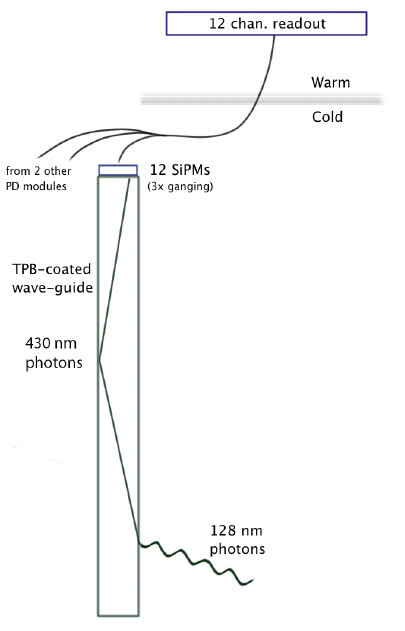
\includegraphics[width=\textwidth]{lightModule.png}
		\caption{}
	\end{subfigure}
	\hfill
	\begin{subfigure}[b]{0.5\textwidth}
		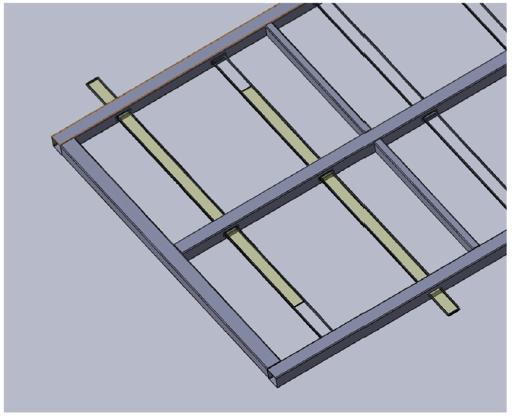
\includegraphics[width=\textwidth]{lightPosition.png}
		\caption{}
	\end{subfigure}
	\caption{\label{lightTPC:fig} (a) Schematic representation of a PD module from the reference design. (b) Positioning of the reference PD modules in the APA frame \cite{DUNE 4}.} 
\end{figure} 

\subsection{FD alternative design: double phase LArTPC }
\begin{figure}
	\centering
	\includegraphics[width=\textwidth]{TPC-Alt.png}
	\caption{\label{TPC-Alt:fig} 3D model of the dual-phase LArTPC atlternative design \cite{DUNE 4}} 
\end{figure}
In addition to the reference design, which has already been chosen as the model for the first FD module, an alternative dual phase design, augmented with a light collection system, is being considered for the other three. In a dual phase LArTPC, the ionization electrons are produced in a tank filled with fully homogenous liquid Argon, then drifted upwards towards an extraction grid  just below a gaseous Argon volume. They are then extracted, amplified via Townsend multiplication and finally collected on a finely segmented anode. This sort of design has several advantages, such as a generally higher gain and consequently a better signal to noise ratio (S/N), a larger fiducial volume, longer drift path and a lower detection threshold. \\
A 100 \% extraction efficiency is achieved applying a 2kV/cm electric field between the extraction grid ( made of stainless steel wires, 1mm in diameter and spaced by 3.125mm ) and the amplification devices placed in ultra pure Argon gas. These devices, called Large Electron Multipliers (LEMs) are 1mm circuit boards placed between two electrodes, micro-patterned with tiny holes. Between the electrodes electron avalanches are induced by applying a 3kV potential difference. It is this feature in particular that improves the S/N ratio by at least an order of magnitude and lowers the threshold for energy deposition, improving resolution. The 2D finely segmented collection anode is placed on top of the gas phase volume and is connected to the first level of electronics.\\
The collection grid, LEM and anode elements are segmented in $0.5\times0.5\ \text{m}^2$
sections and combined to form independent modules called Charge readout PLANES (CRPs), which are embedded in a FR-4 and stainless steel armour. These are suspended from the roof of the tank and cover the entire upper surface. Combined with PMT arrays, collecting the scintillation light for timing information, a CRP module provides 3D position and calorimetric reconstruction. A schematic representation of these elements is shown in Figure \ref{CRP:fig}.\\
The cathode layer, that produces the drift field ($E_{drift}\sim$ 0.5 kV/cm) covers the tank's floor. The field is kept homogenous by a field-cage, comprised of a stack of 60 field-shaping electrodes of decreasing voltage from bottom to top. The design is completed by the external cryostat and signal feed-through elements called chimneys, which put in contact the internal electronic with the outside of the tank. A 3D module of the entire structure is shown in Figure \ref{TPC-Alt:fig}.  
\clearpage
\begin{figure}
	\centering
	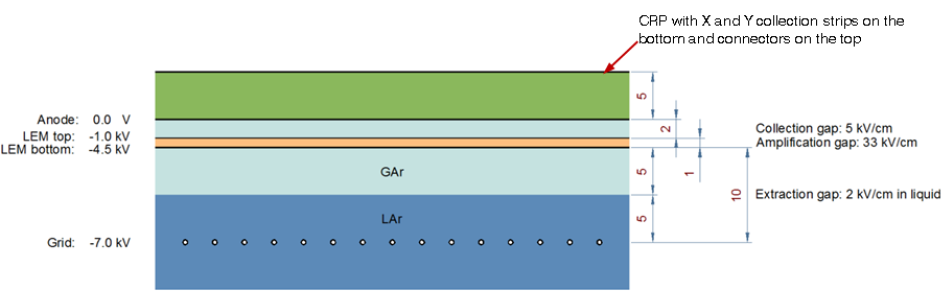
\includegraphics[width=\textwidth]{CRP.png}
	\caption{\label{CRP:fig} Schematic representation of a CRP module with thickness and voltage vales for a 0.5 kV/cm drift field in liquid Argon\cite{DUNE 4}. } 
\end{figure}
\subsection{The near detector}
The near detector will be located in the Fermilab facilities a few hundred meters away from the beam source. It will constitute of two movable systems, capable of being positioned both on and off-axis, and a fixed one that will always be on axis. The two movable detectors will both be based on Argon as a target, an essential characteristic for evaluating the systematics on the Far detector's physics response. One of them will contain liquid Argon, while the other will be based on a high pressure gas Argon TPC technology. \\
The liquid argon TPC will be called ArgonCube and will feature a modular design and a fully pixelated charge readout \cite{ArgonCube}. The advantages of segmenting a large LArTPC are a reduction in drift voltage requirements and a lessened focus on Argon purity. This in turn reduces risks related to electric breakdown and purity losses. The pixelated charge readout provides an unambiguous event topology reconstruction, which is vital in cases of events with high multiplicity and possibility of pile-up. In Figure \ref{ArgonCube:fig} a geometric representation of ArgonCube with a cross section of one of its modules is presented.\\
The second movable detector, HPgTPC (High Pressure gas TPC) is a magnetized spectrometer based on high pressure gas Argon TPC technology, surrounded by an electro-magnetic calorimeter \cite{HPgTPC}. Its main purpose will be to tag muons and the sign of charged particles exiting ArgonCube, thanks to its optimal tracking efficiency, particle identification and momentum and angular resolution. HPgTPC will also be extremely useful in detecting charged particles of very low energy from $\nu$ interactions in gas.  \\
The fixed detector will reuse parts of a previous detector named KLOE, today situated at the Laboratori Nazionali di Frascati (LNF) and will take the name SAND (System for on-Axis Neutrino Detection) \cite{KLOE}. The specific purpose of this detector in its Straw Tube Tracker (STT) configuration, one of the two currently being considered, will be discussed in Chapter 3 \cite{SAND}.
\begin{figure}[t]
	\centering
	\begin{subfigure}[b]{0.475\textwidth}
		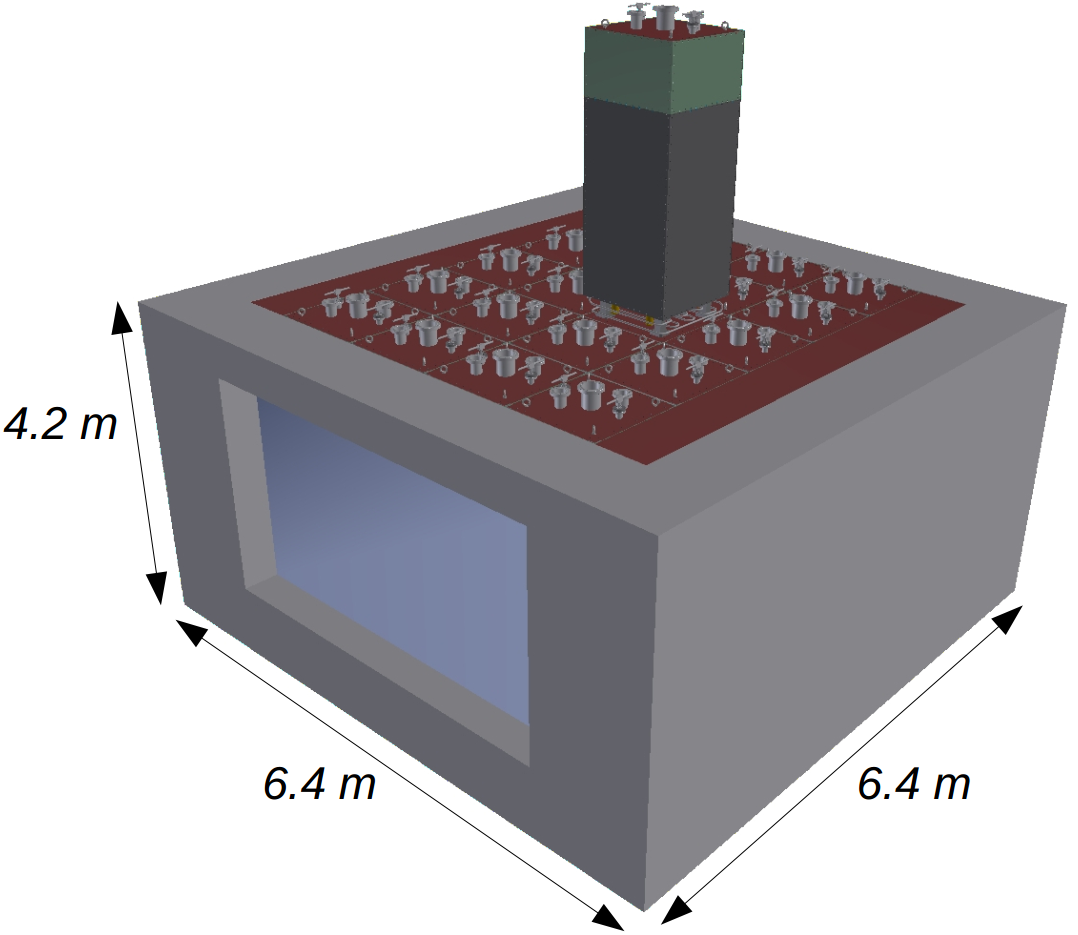
\includegraphics[width=\textwidth]{ArgonCube.png}
		\caption{}
	\end{subfigure}
	\hfill
	\begin{subfigure}[b]{0.475\textwidth}
		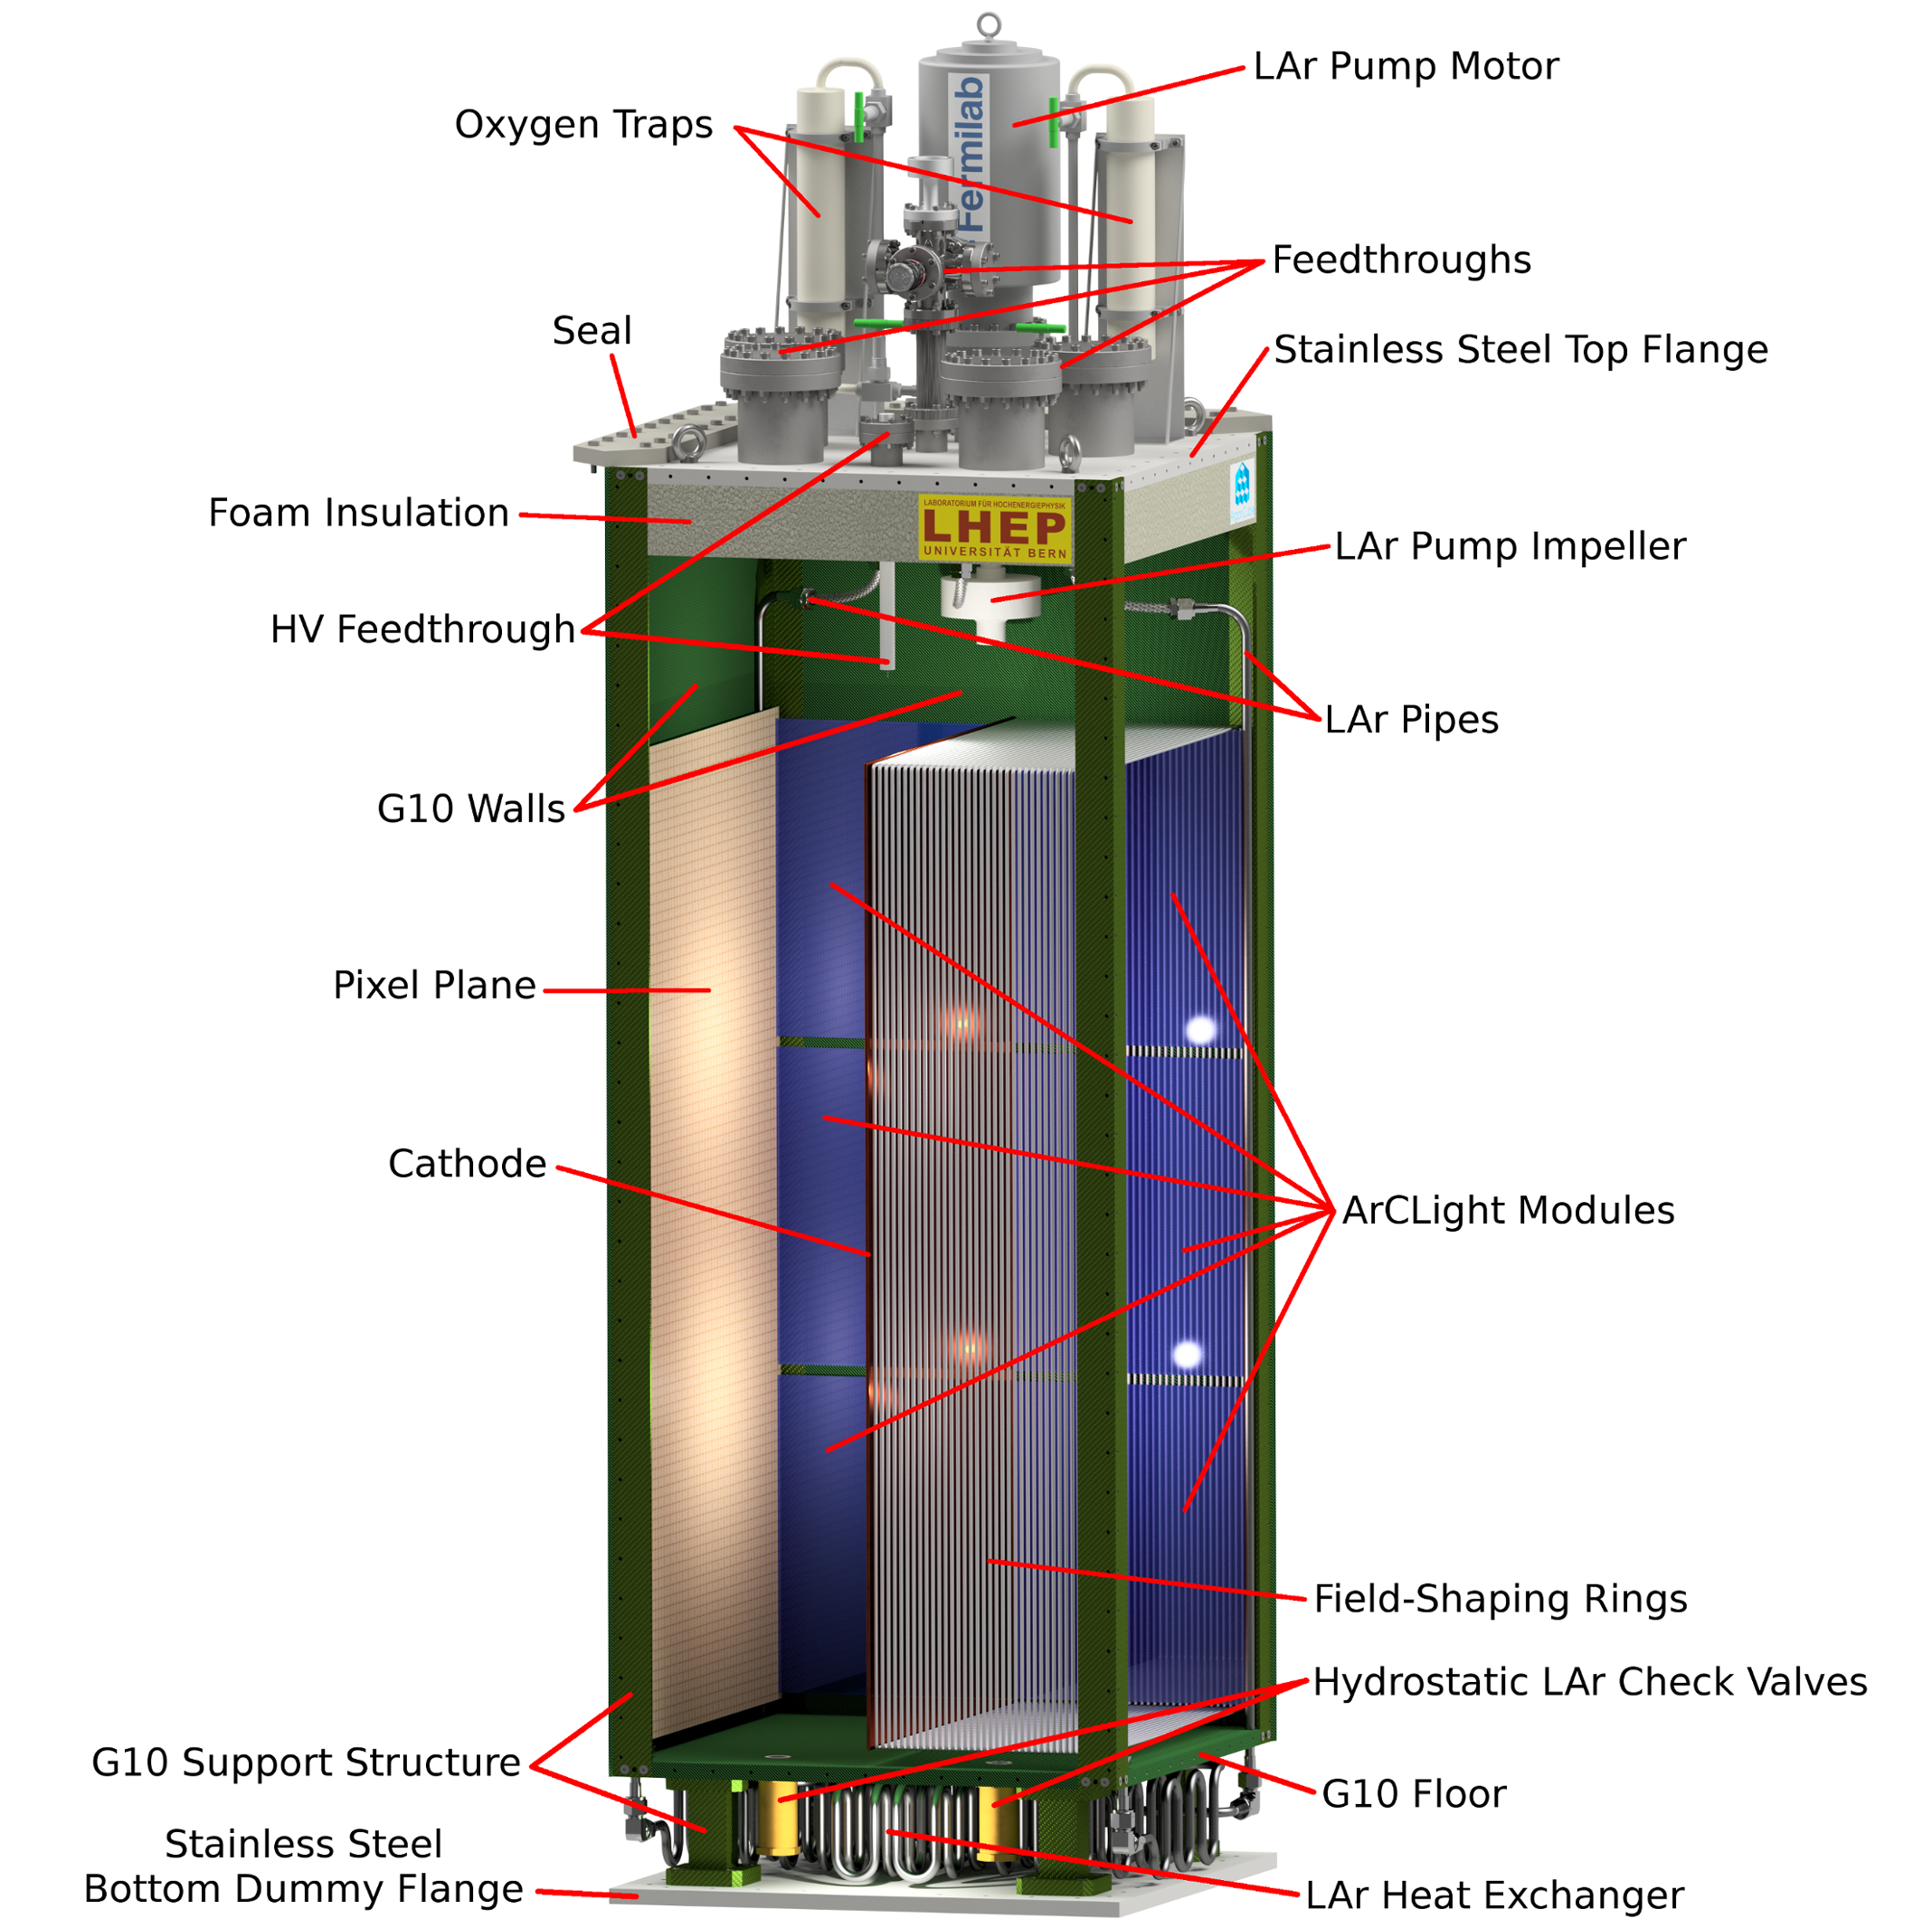
\includegraphics[width=\textwidth]{ArgonCubeModule.png}
		\caption{}
	\end{subfigure}
	\caption{\label{ArgonCube:fig} Schematic design of the ArgonCube liquid argon detector (a) and one of its modules (b) \cite{ArgonCube images}} 
\end{figure}

\section{DUNE' s scientific program}

The scientific objectives of DUNE are categorized into a $primary$ and an $ancillary$ scientific programme \cite{DUNE symmetries}. The latter is further divided into secondary objectives that could be persued by the experiment just by virtue of how it will be built and additional secondary objectives that may require specific upgrades to the facility.\\
The \emph{primary} programme is made up by the main measurements that DUNE will be built to perform with unprecedented precision which coincide with the fundamental questions that this experiment will try to answer:
\begin{enumerate}
	\item \textbf{Measurement of the charge-parity violating phase $\delta_{CP}$ and determination of the mass ordering of the neutrinos} (i.e. the sign of $\Delta m^2_{31}=m_3^2-m_1^2$). The study of $\delta_{CP}$ is particularly important in cosmological models trying to explain the matter-antimatter asymmetry in the universe.
	\item \textbf{Precision measurements of the $\nu_\mu \rightarrow \nu_{\mu,e}$ oscillation parameters}: the $\theta_{13}$ mixing angle; the $\theta_{23}$ mixing angle and the octant it lies in; the value of the $|\Delta m_{32}^2|$  mass difference. Precision measurements of these parameters and comparisons with corresponding patterns in the quark sector will further our knowledge of the underlying symmetries in fundamental particle physics.
	\item \textbf{Search for proton decay in one or more decay modes, improving significantly on previous lifetime limits}. Most Grand Unified Theories (GUTs) make lifetime predictions for nucleons and putting more and more stringent limits will be fundamental in assessing which one of them might be correct.
	\item \textbf{Detection and measurements of the neutrino flux from a core-collapse supernova}. In particular the time structure and energy spectrum of the neutrino burst would much further our understanding of this astrophysical phenomenon.
\end{enumerate}

The \emph{ancillary} programme consists of objectives that DUNE is not specifically conceived to achieve, but that are nonetheless enabled by the facility's design:
\begin{enumerate}
	\item Further accelerator oscillation measurements and search for non-standard interactions Beyond the Standard Model (BSD)
	\item Atmospheric neutrino oscillation measurements
	\item Measurements of other astrophysical phenomena using moderate energy neutrinos
\end{enumerate}
Finally the \emph{additional secondary} programme includes measurements potentially made possible by future upgrades to the facility such as monitoring of the diffuse supernova flux, solar neutrino and other low energy astrophysical neutrino measurements.\\
The characteristics required by the \emph{DUNE Near Detector (ND)} will also allow it to have a scientific programme of its own. Its main objective will be to perform all the precision measurements necessary to achieve the goals of the primary programme. It will also pursue precision studies of the weak interaction, studies of nuclear and nucleon structure and searches for new physics. 

\subsection{Sensitivities and systematics} 

In order to make any precision measurement one should be acutely aware of the systematic uncertainties related to the analysis strategy and the performance of the detector. To alleviate the impact of the systamatic effects on the results, most Long Baseline neutrino experiments uses two detectors at different sites (FAR and NEAR). In these experiments the $\nu_\mu$ spectrum measured in the Near Detector $N_{ND}^{data}(\nu_\mu)$ is propagated to the Far Detector and is used to predict the expected signal of $\nu_\mu$ and oscillated $\nu_e$ (and much smaller component of oscillated $\nu_\tau$) i.e. $N_{FD}^{exp}(\nu_\mu)$ and $N_{FD}^{exp}(\nu_e)$. Likewise the $\nu_e$ measured spectrum in the ND, mostly comprised of electron neutrinos from the beam and misidentified NC $\pi^0$ is used to predict the background at the FD. \\
The measured neutrino spectrum at the near detector is given by:
\begin{equation}
N_{ND}^{data}(\nu_{\mu,e})= \Phi_{ND}(\nu_{\mu,e}) \otimes \varepsilon_{ND}(\nu_{\mu,e}) \otimes \sigma_{ND}(\nu_{\mu,e})
\end{equation}
where $\Phi_{ND}(\nu_{\mu,e})$ is the beam flux, $\varepsilon_{ND}(\nu_{\mu,e})$ is the detector's efficiency and $\varepsilon_{ND}(\nu_{\mu,e})$ is the neutrino interaction cross section. In order to use such data to predict the signal and background expected at the far detector one needs to take into consideration:
\begin{itemize}
	\item \emph{Differences in how the neutrino interact $\sigma_{FD}/\sigma_{ND}$.} These are null in the case that the target nuclei in the Near and Far Detector are the same. Otherwise the dominating uncertainties in the prediction of $\nu_e$ in FD from measurement of $\nu_\mu$ in ND are the ones arising from differences in the electronic and muonic cross sections between the detectors: $\sigma_{FD}(\nu_e)/\sigma_{ND}(\nu_\mu)$.
	\item \emph{Differences in detector efficiencies $\varepsilon_{FD}/\varepsilon_{ND}$.} These uncertainties mostly arise from the differences in event selection between the two detectors and in particular the modelling of the energy scales. These are also virtually inexistent in the case that ND and FD are identical.
	\item \emph{Differences in the neutrino flux $\Phi_{FD}/\Phi_{ND}$.} The fluxes at the Near and Far detector are radically different since the ND is very close to the beamline and sees an expanded source, while the FD is 1300 km away. A Monte Carlo is used to simulate the beam propagation, but it is itself not immune from inaccuracies: errors in the hadron production, focusing of the horns composition of the beam pipe and decay channel geometry can all contribute. 
\end{itemize} 
\begin{figure}[t!]
	\centering
	\renewcommand{\figurename}{Table}
	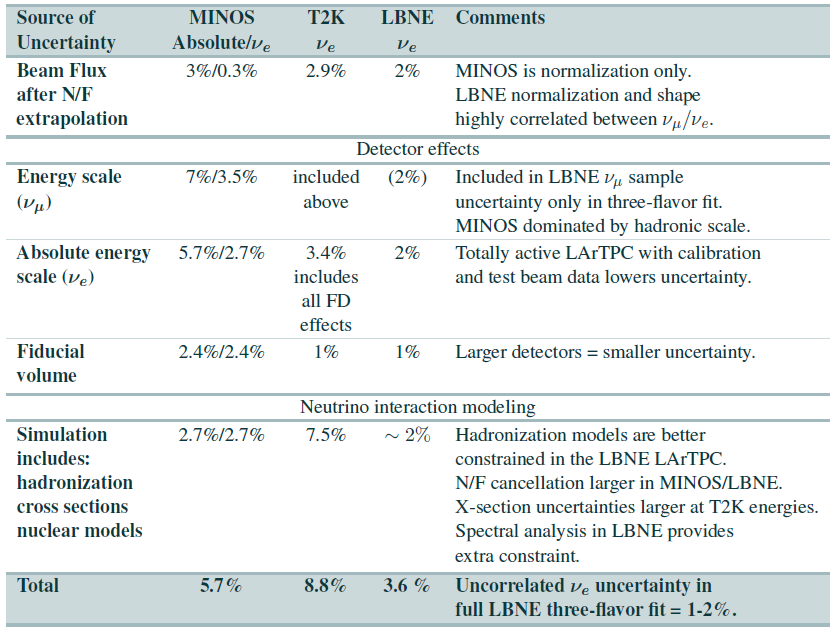
\includegraphics[width=0.75\textwidth]{uncertainties.png}
	\caption{\label{uncertainties:fig} Dominant systematics on the $\nu_e$ appearence channel for T2K and MINOS and projection for LBNE (Long Baseline Neutrino Experiment), the preliminary name used for DUNE. \cite{DUNE symmetries}} 
\end{figure}
The $\nu_\mu$ expected signal is given by:
\begin{equation}
N_{FD}^{exp}(\nu_\mu) = N_{ND}^{data}(\nu_\mu) \otimes \frac{\Phi_{FD}(\nu_\mu)}{\Phi_{ND}(\nu_\mu)} \otimes P(\nu_\mu \rightarrow \nu_\mu) \otimes \frac{\varepsilon_{FD}(\nu_\mu)}{\varepsilon_{ND}(\nu_\mu)} \otimes \frac{\sigma_{FD}(\nu_\mu)}{\sigma_{ND}(\nu_\mu)} 
\end{equation}
The $\nu_e$ expected signal is given by:
\begin{equation}
\begin{split}
N_{FD}^{exp}(\nu_e) & = \underbrace{N_{ND}^{data}(\nu_\mu) \otimes \frac{\Phi_{FD}(\nu_\mu)}{\Phi_{ND}(\nu_\mu)} \otimes P(\nu_\mu \rightarrow \nu_e) \otimes \frac{\varepsilon_{FD}(\nu_e)}{\varepsilon_{ND}(\nu_\mu)} \otimes \frac{\sigma_{FD}(\nu_e)}{\sigma_{ND}(\nu_\mu)}}_{\text{Expected signal}} \\
& + \underbrace{N_{ND}^{data}(\nu_e) \otimes \frac{\Phi_{FD}(\nu_e)}{\Phi_{ND}(\nu_e)} \otimes P(\nu_e \rightarrow \nu_e) \otimes \frac{\varepsilon_{FD}(\nu_e)}{\varepsilon_{ND}(\nu_e)} \otimes \frac{\sigma_{FD}(\nu_e)}{\sigma_{ND}(\nu_e)}}_{\text{Electronic events from the beam}} \\
& + \pi^0\text{NC background prediction from }N_{ND}^{data}(\nu_e)\\
& + \nu_\tau \text{ background prediction from }N_{ND}^{data}(\nu_\mu)
\end{split}
\end{equation}
The main sources of uncertainties are known from previous experiments such as T2K and MINOS. They include:
\begin{itemize}
	\item \emph{Beam flux uncertainties}: related to the precision with which the ND is capable to measure the unoscillated beam flux in both shape and normalization.
	\item \emph{$\nu_\mu$ energy-scale uncertainties}: the muonic neutrino energy spectrum measured in the ND is used to predict the $\nu_e$ appearance channel in the FD.
	\item \emph{Absolute $\nu_e$ energy-scale uncertainty}: an accurate measurement of the spectral shape of the $\nu_e$ appearance channel at the ND, is essential to obtain a high MH and CP-violation sensitivity. The determination of the electron neutrino energy is influenced by the detector response, which introduces important systematic uncertainties in the absolute $\nu_e$ energy scale. 
	\item \emph{Simulation uncertainties}: uncertainties related to the modelling of the neutrino interactions with the target nuclei in the near and far detectors.
\end{itemize}
In Table \ref{uncertainties:fig} the dominant uncertainties for $\nu_e$ appearance for the T2K and MINOS and a preliminary prediction for DUNE are summarized. The precision is expected to improve from all fronts.


\begin{figure}[t!]
	\centering
	\includegraphics[width=0.85\textwidth]{oscillograms.png}
	\caption{\label{oscillograms:fig} $\mathcal{A}_{CP}$ total asymmetry as a function of baseline and energy. The top two oscillograms show the asymmetry for $\delta_{CP}=0$ (i.e. $\mathcal{A}_{matter}$) for Normal (left) and Inverted (right) mass ordering. The two bottom oscillograms show the asymmetry in vacuum (i.e. $\mathcal{A}_{\delta}$) for $\delta_{CP}=\pi/2$ (left) and $\delta_{CP}=-\pi/2$ (right). DUNE's baseline (1300km) and the 1st and 2nd oscillation nodes are highlighted in black \cite{DUNE 2}. } 
\end{figure}
\subsection{Mass ordering and $\delta_{CP}$}
As it can be seen from Eq. \ref{eq:asymmetry} both a non-zero $\delta_{CP}$ and matter effects can induce asymmetries between $P(\nu_\mu \rightarrow \nu_e)$ and $P(\bar{\nu}_\mu \rightarrow \bar{\nu}_e)$and thus:
\begin{equation}
\mathcal{A}_{CP}= \mathcal{A}_{\delta}+ \mathcal{A}_{matter}
\end{equation}
In figure \ref{oscillograms:fig} the asymmetries induced by CP violation ($\mathcal{A}_{\delta}$) in case that $\delta_{CP}=\pm\pi/2$ and by matter effects ($\mathcal{A}_{matter}$) are plotted separatly in 2D oscillograms as a function of baseline and energy. In reality though the two asymmetries are never separated. In experiments where both are relevant, as is the case for DUNE, if one wants to use  measurements of total asymmetry both to measure $\delta_{CP}$ and the mass ordering, it's mandatory to be able to disambiguate between the two \cite{DUNE 2}. \\
For the MSW effects in particular the asymmetries are introduced by a CP violating term $P_{\sin\delta}$ in the oscillation probability:
\begin{equation}
P(\nu_\mu \rightarrow \nu_e) \simeq P(\nu_e \rightarrow \nu_\mu) \simeq P_0+P_{\sin\delta}+P_{\cos\delta}+P_3
\end{equation}
where
\begin{equation}
P_0=\sin^2\theta_{23}\frac{\sin^22\theta_{13}}{(A-1)^2}\sin^2[(A-1)\Delta]
\end{equation}
\begin{equation}
P_3=\alpha^2\cos^2\theta_{13}\frac{\sin^22\theta_{12}}{A^2}\sin^2(A\Delta)
\end{equation}
\begin{equation}
P_{\sin\delta}=\alpha\frac{8J_{CP}}{A(1-A)}\sin\Delta\sin(\Delta A)\sin((1-A)\Delta)
\end{equation}
\begin{equation}
P_{\cos\delta}=\alpha\frac{8J_{CP}\cot \delta_{CP}}{A(1-A)}\sin\Delta\sin(\Delta A)\sin((1-A)\Delta)
\end{equation}
with 
\begin{equation}
\Delta = \Delta m_{31}^2 L/4E
\end{equation}
\begin{equation}
A=\sqrt{3}G_FN_e2E/\Delta m_{31}^2
\end{equation} 
\begin{equation}
\alpha = |\Delta m_{12}^2 |/|\Delta m_{31}^2 |
\end{equation}
\\
Note that since the value of $\Delta m_{31}^2$ switches between normal and inverted hierarchy, the asymmetry effects induced by the passage through matter will also be different: for normal (inverted) hierarchy $P(\nu_\mu-\nu_e)$ is enhanced (suppressed) and $P(\bar{\nu}_\mu\rightarrow\bar{\nu}_e)$ is suppressed (enhanced); 
the matter effects shift the phase of oscillation pattern for a fixed baseline to lower energies (by about -100 MeV) in the IH. \\
In general the matter effects have the largest impacts when the oscillation nodes for $\theta_{13}$ are reached (the first two nodes are highlighted in black in Figure \ref{oscillograms:fig}):
\begin{equation}
\frac{L(\text{km})}{E(\text{GeV})} = (2n-1)\frac{\pi}{2}\frac{1}{(1.27\times\Delta m_{31}^2(\text{eV}^2))} \simeq(2n-1)\times 510 \ \text{km/GeV}
\end{equation}
\begin{figure}[t!]
	\centering
	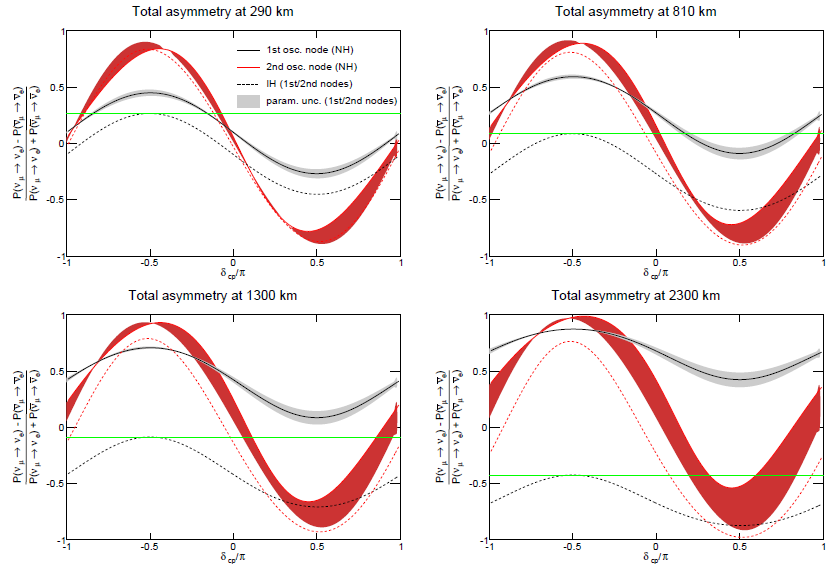
\includegraphics[width=0.8\textwidth]{asymmetrydelta.png}
	\caption{\label{asymmetrydelta:fig} Total $\mathcal{A}_{CP}$ as a function of $\delta_{CP}/\pi$ for four different baselines (290 km, 810 km, 1300 km and 2300 km). The black (red) lines indicate the asymmetries at the first (second) node, the full ones being for NH and the dashed ones for IH \cite{DUNE 2}. } 
\end{figure}
For an experiment such as DUNE, where we have a baseline of $L\sim1300$ km (highlighted in black in Figure \ref{oscillograms:fig}) and an energy range $E\sim5-10$ GeV, the matter effects are maximal, and it is then crucial that they are disentangled from the CP effects.\\
Knowing the value of $|\Delta m_{31}^2 |$ (only the sign is still unknown), one can see, though, that for a baseline $>$ 1200km, the size of $\mathcal{A}_{matter}$ surpasses the highest possible value of $\mathcal{A}_{\delta}$ which makes the disambiguation between the two effects possible. In Figure \ref{asymmetrydelta:fig} the plots show the total asymmetry at the first (black) and second (red) nodes as a function of $\delta_{CP}$ for four different values of $L$: 290 km, 810 km, 1300 km (baseline of DUNE) and 2300 km. Depending on the hierarchy asymmetries will have different values because of the matter effects and are plotted as full and dashed lines respectively. As the baseline gets bigger, given the same node, the CP-induced asymmetry will stay the same while matter induced one will get bigger since the dependencies on $L$ and E are:
\begin{equation}
\mathcal{A}_{\delta} \propto L/E
\end{equation}
\begin{equation}
\mathcal{A}_{matter} \propto L\times E
\end{equation}
If one considers then the case in which the $\delta_{CP}$ asymmetries is maximal (green line in the plots) is easy to see that if $\mathcal{A}_{matter} < \mathcal{A}_\delta^{max}$ the same total asymmetry is compatible with both hierarchies and multiple value of $\delta_{CP}$. This is true for baselines shorter than 1200km. For DUNE, where $L\sim1300$km these ambiguities don't exist.

\subsubsection{Significance for mass ordering and $\delta_{CP}$ measurements}
The sensitivity with which the DUNE experiment will be able to measure the mass ordering (MO) and CP-Violation (CPV), is evaluated by fitting the simulated oscillation spectra of $\nu_\mu \rightarrow \nu_{\mu,e}$ and $\bar{\nu}_\mu \rightarrow \bar{\nu}_{\mu,e}$ for different values of the oscillation parameters and confronting the results with the expected theoretical values in terms of $\Delta\chi^2$:
\begin{equation}
\Delta\chi^2_{MO}= |\chi^2_{MH^{test}=IH}-\chi^2_{MH^{test}=NH}| 
\end{equation}
\begin{equation}
\Delta\chi^2_{CPV}= \min (\Delta\chi^2_{CP}(\delta_{CP}^{test}=0),\Delta\chi^2_{CP}(\delta_{CP}^{test}=\pi))
\end{equation}
with $\Delta\chi^2_{CP}=\chi^2(\delta_{CP}^{test})-\chi^2(\delta_{CP}^{true})$. The significance with which DUNE will be able to assess the mass ordering grows with the exposure, defined as kt of active volume $\times$ MW beam power $\times$ years, and varies wildly with the value of $\delta_{CP}$ (Figure \ref{exposure-MO:fig}). In order to ensure the DUNE objective of reaching $\sqrt{\Delta\chi^2}=5$ for every value of $\delta_{CP}$ approximately an exposure of 200-400 kt$\times$MW$\times$years will be needed. The significance for $\delta_{CP}$ similarly grows with exposure (Figure \ref{exposure-deltaCP:fig}), apart from 0 and $\pi$. The significance for both MO and CPV also depends strongly on the values of all the other oscillation parameters (Figure \ref{MOsignificance-param:fig} and \ref{CPVsignificance-param:fig}), making precision measurements with DUNE mandatory.
\clearpage
\begin{figure}
	\centering
	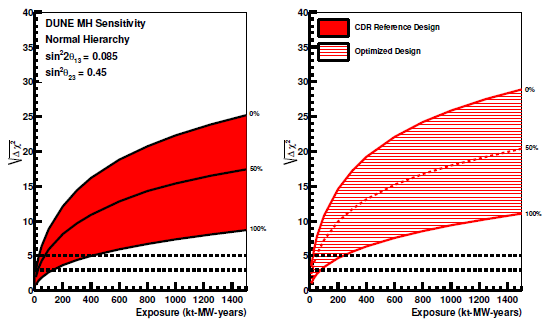
\includegraphics[width=0.6\textwidth]{exposure-MO.png}
	\caption{\label{exposure-MO:fig} MO significance as a function of exposure for two different beam designs (left and right) and three values of CP asymmetry (0\%,50\%,100\%) \cite{DUNE 2}. } 
\end{figure}
\begin{figure}
	\centering
	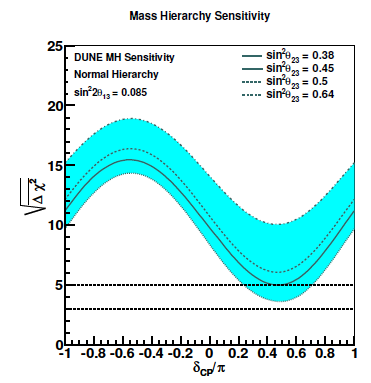
\includegraphics[width=0.375\textwidth]{MOVStheta23.png}
	\qquad
	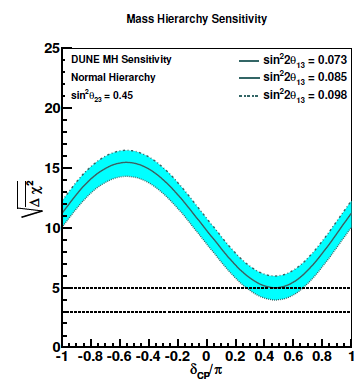
\includegraphics[width=0.375\textwidth]{MOVStheta13.png}
	\qquad
	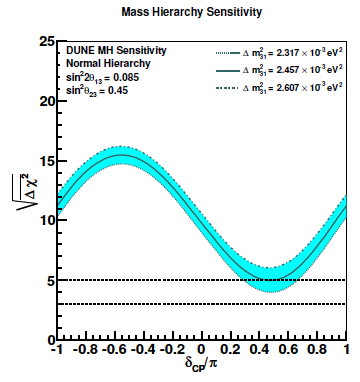
\includegraphics[width=0.375\textwidth]{MOVSm31.png}
	\caption{\label{MOsignificance-param:fig} MO significance as a function of $\delta_{CP}/\pi$ at a fix value of exposure 300 kt$\times$MW$\times$years for different values of the oscillation parameters: $\theta_{23}$ (upper-left), $\theta_{13}$ (upper-right), $\delta m_{31}^2$ (bottom) \cite{DUNE 2}.} 
\end{figure}

\begin{figure}
	\centering
	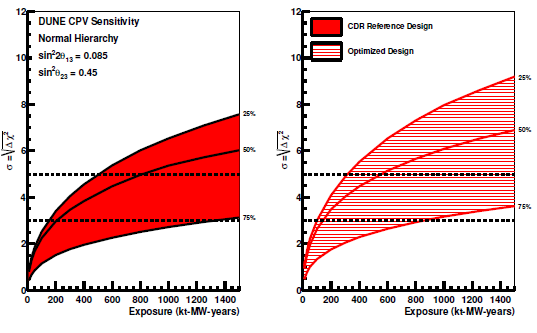
\includegraphics[width=0.58\textwidth]{exposure-CPV.png}
	\caption{\label{exposure-deltaCP:fig} CPV significance as a function of exposure for two different beam designs (left and right) and three values of CP asymmetry (0\%,50\%,100\%). \cite{DUNE 2} } 
\end{figure}
\begin{figure}
	\centering
	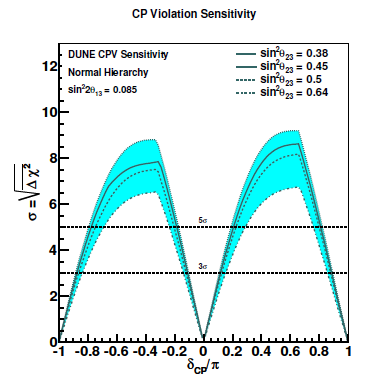
\includegraphics[width=0.375\textwidth]{CPVVStheta23.png}
	\qquad
	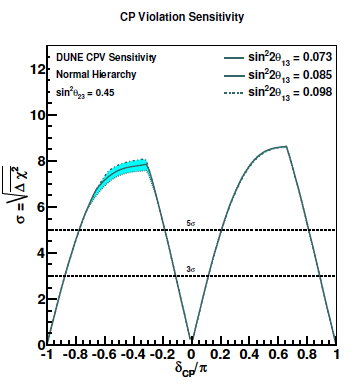
\includegraphics[width=0.375\textwidth]{CPVVStheta13.png}
	\qquad
	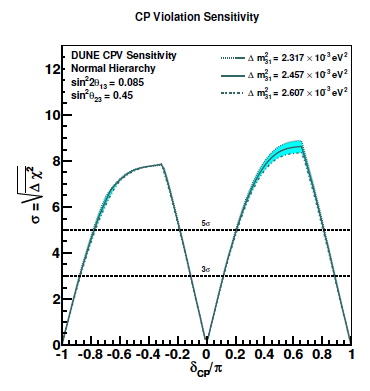
\includegraphics[width=0.375\textwidth]{CPVVSm31.png}
	\caption{\label{CPVsignificance-param:fig} CPV significance as a function of $\delta_{CP}/\pi$ at a fix value of exposure 300 kt$\times$MW$\times$years for different values of the oscillation parameters: $\theta_{23}$ (upper-left), $\theta_{13}$ (upper-right), $\delta m_{31}^2$ (bottom) \cite{DUNE 2}.} 
\end{figure}
\clearpage
\subsection{Precision measurements}
\begin{figure}
	\centering
	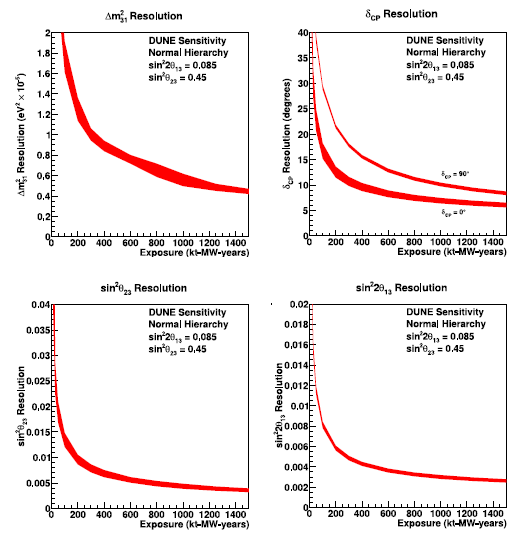
\includegraphics[width=0.6\textwidth]{precision.png}
	\caption{\label{precision:fig} Resolution as a function of exposure for $\Delta m_{31}^2$ (upper left), $\delta_{CP}$ (upper right), $\sin^2\theta_{23}$ (bottom left) and $\sin^2\theta_{13}$ (bottom right). The red area represents the range in sensitivity due to differences in beam design \cite{DUNE 2}. } 
\end{figure}
The DUNE experiment will improve sensitivity on the key parameters governing $\nu_\mu-\nu_\mu$ and $\nu_\mu-\nu_e$: 
\begin{itemize}
	\item $\sin^2\theta_{23}$ and the octant of $\theta_{23}$;
	\item$\delta_{P}$; \item$\sin^2\theta_{13}$;
	\item$\Delta m_{31}^2$.
\end{itemize}
The sensitivity to these parameters as a function of exposure is plotted in Figure \ref{precision:fig} \\
Determining the octant of the mixing angle $\theta_{23}$, and thus if its value is exactly $45^\circ$ producing maximal mixing between mass eigenstates 2 and 3 is still an open question, with the latest results from T2K leaving both a lower ($<45^\circ$) and upper ($<45^\circ$) octant scenarios open, depending on the mass hierarchy being considered. This particular question is of great theoretical interest. A value of $\theta_{23}$ being exactly $45^\circ$ would hint at new not yet considered symmetries, while for example an excess in the upper octant of the order of the Cabibbo angle, point in the direction of quark-lepton universality models. \\
The measurement of the octant is made possible by combining survival ($\nu_\mu \rightarrow \nu_\mu$) and disappearance ($\nu_\mu \rightarrow \nu_e$) probabilities, the first being sensitive to $\sin^22\theta_{23}$ an the second to  $\sin^2\theta_{23}$. The $\Delta\chi^2$ for the determination of the octant is then:
\begin{equation}
\Delta\chi^2_{octant}=|\chi^2_{\theta_{23}>45^\circ}- \chi^2_{\theta_{23}<45^\circ}|
\end{equation}
The sensitivity to the octant as a function of $\theta_{23}$ is plotted in Figure\ref{octant:fig}.\\
DUNE will also be able to perform unitarity tests of the PMNS matrix by measuring precisely the value of $\sin2\theta_{13}$, which will constrain the phase space of possible new physics. In general the high precision measurement performed by DUNE could reveal new physics driven for example by non-standard interactions or the existence of sterile neutrinos.
\begin{figure}[t!]
	\centering
	\includegraphics[width=0.6\textwidth]{octant.png}
	\caption{\label{octant:fig} $\Delta\chi^2_{octant}$ as a function of $\theta_{23}$. The yellow areas indicate the $1\sigma$ and $3\sigma$ intervals for the value of $\theta_{23}$ from recent global fits. The green area represents the range in sensitivity due to differences in beam design and $\delta_{CP}$ value \cite{DUNE symmetries}.} 
\end{figure}  
\subsection{Proton decay measurements}
\begin{figure}
	\centering
	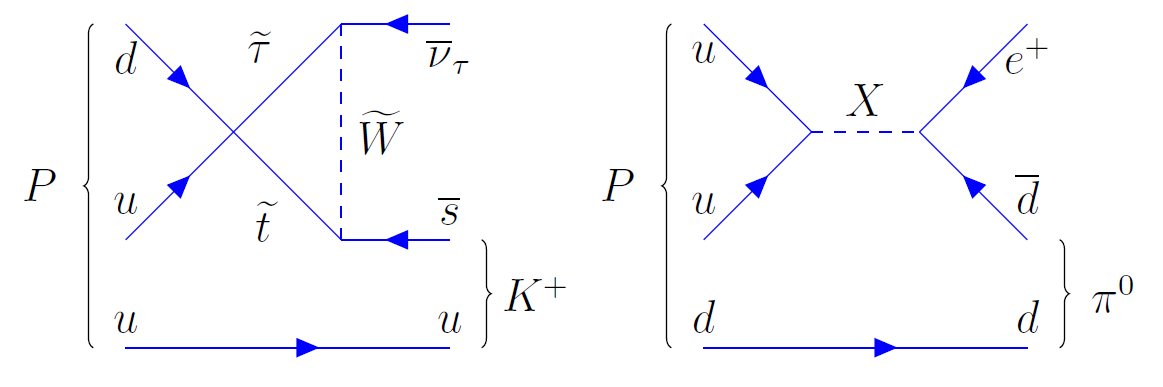
\includegraphics[width=\textwidth]{ProtonDecay.png}
	\caption{\label{ProtonDecay:fig} Feynman diagrams for two major proton decay modes: the main decay for SUSY GUTs $p^+\rightarrow K^+ \bar{\nu}$ (left) and the main decay for gauge-mediation GUTs $p^+\rightarrow e^+ \pi^0$ (right)\cite{DUNE symmetries}.} 
\end{figure}
Almost all Grand Unified Theories (GUTs) predict proton decay and baryon number non conservation. Detecting a proton decay would be in fact one of the only viable experimental strategies to probe these theories since the unification scale is in excess of about $10^{15}$ GeV with respects to energies accessible to accelerator experiments.\\
The non-detection of proton decay sets proton life-time constraints and progressively rules out theories based on their predictions. The most recent limits set by Super-Kamiokande have in fact confirmed the ruling out of minimal SU(5) (previously established by IMB and Kamiokande) and has disproved minimal SUSY SU(5). The next generation of large underground experiments such as Hyper-Kamiokande and DUNE will be well equipped to continue the search and, at the very least, make the constraints more stringent.\\
From the theoretical body of work, two main decay mode emerge, the first from supersymmetric GUTs and the second from gauge-mediated GUTs (see Figure \ref{ProtonDecay:fig} for the Feynmann diagrams):
\begin{equation}
p^+ \rightarrow K^+ \bar{\nu}
\end{equation}
\begin{equation}
p^+ \rightarrow e^+ \pi^0
\end{equation}
The first decay mode is especially interesting for large LArTPCs (such as the FD of DUNE) since it presents a kaon in its final state: kaons have an especially high ionization rate and would be detected with great efficiency using liquid Argon technologies. The second one is perhaps better known and has its most clear signature in Cherenkov detectors, since it consists of an electromagnetic shower ignited by the the $e^+$ and two $\gamma$ from the $\pi^0$ decay.
\subsection{Supernova neutrino measurements}
\begin{figure}
	\centering
	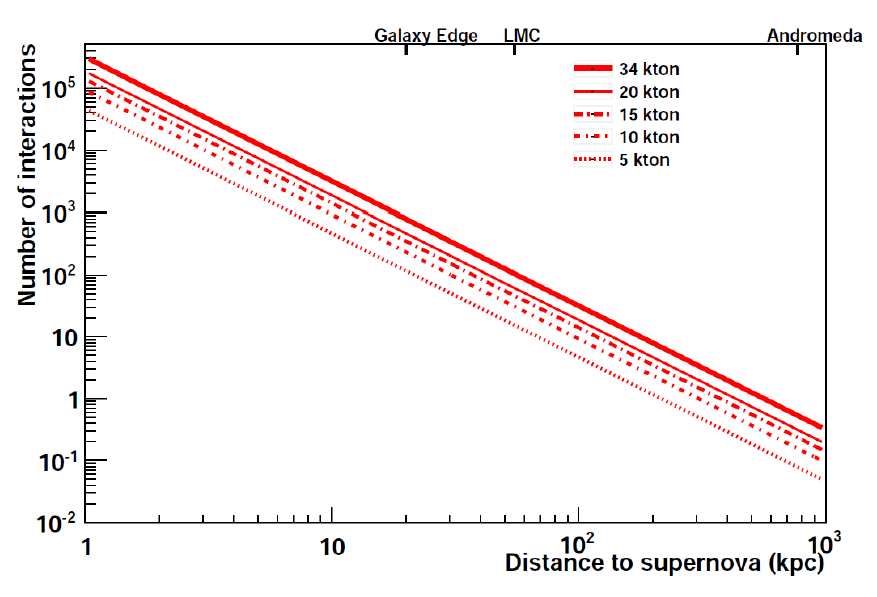
\includegraphics[width=0.7\textwidth]{Supernova.png}
	\caption{\label{Supernova:fig} Number neutrino interactions from supernova explosions, as a function of distance, for different volume LArTPCs \cite{DUNE symmetries}.} 
\end{figure}
Given an experimental life of 20 years, DUNE would have about a 40\% chance of observing neutrinos from a core collapse Supernova in the Milky Way. This would be of great importance for our understanding of this astrophysical phenomenon, which has only been confirmed in its basic characteristics by the observation of neutrino events from SN1987, a supernova in the Large Magellanic Cloud, 50 kpc away. \\
Supernovas also promise an extremely varied environment to study neutrino oscillation, with their initial flavour composition being strictly linked to the expanding shock and turbulence. For example the oscillation patterns would be very different for NH and IH. The oscillations of neutrinos and anti-neutrinos would also manifest rather differently, making the observation of both with high statistics of particular interest.\\
LArTPCs are sensitive to $\nu_e$, due to the absorption channel on Argon:
\begin{equation}
\nu_e+ ^{40}\text{Ar} \rightarrow e^- + ^{40}\text{K}^*
\end{equation}
This interaction can be in principle detected exploiting the coincidence of the gamma cascade produced by the de-excitation of $^{40}$K$^*$ and the electron. The plot in Figure \ref{Supernova:fig} shows the number neutrino interactions from supernova explosions, as a function of distance, for LArTPCs of different volumes. For a detector of 10 kt, about the size of the FD of DUNE, a Supernova explosion at the likely distance of about 10 kpc would produce about 900 events. Only 19 events from two Cherenkov detectors and a few more from scintillation detectors were registered for SN1987A.
\subsection {Oscillation physics with atmospheric neutrinos}
A module of the DUNE's Far Detector, given its 10 kt mass and being $\sim1500$ m underground, will be well equipped to perform oscillation measurements using atmospheric neutrinos. Given that the atmospheric sample contains $\nu$'s of all flavours over a vast range of energy and path lengths, including some for which matter effects are relevant, all oscillation parameters could be measured, offering a very useful complementary program to the main accelerator one. \\
Measuring atmospheric oscillations would also be very useful in the field of mass ordering determination. Additionally it offers an alternative method of measuring $\theta_{23}$ and its octant.Finally, new physics searches are also possible in the atmospheric sector.
\begin{figure}
	\centering
	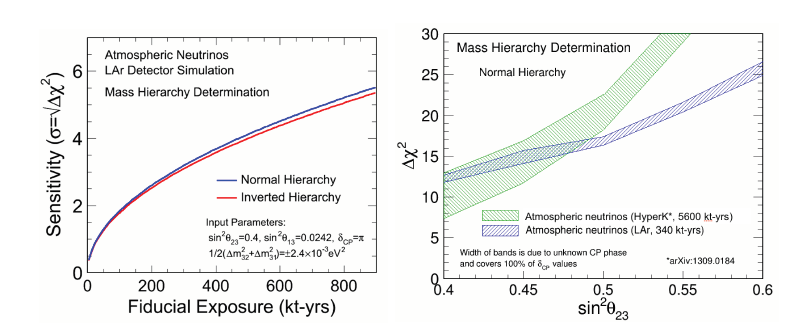
\includegraphics[width=\textwidth]{DUNEatm.png}
	\caption{\label{DUNEatm:fig}(\emph{Left}) MO sensitivity for the atmospheric neutrino sample as a function of exposure for both NH (blue) and IH (red); (\emph{Right}) MO sensitivity for the atmospheric neutrino sample as a function of the true value of $\theta_{23}$ in NH, with values for Hyper-K given for comparison. \cite{HYperk Physics}} 
\end{figure} 

\subsection{Near detector physics}
The Near detector main goal is to provide a precise characterization of the neutrino flux and its energetic spectrum and flavour composition, which is mandatory to make predictions on the far/near flux ratio.\\
Since the near detector will collect a high statistics sample of neutrino interactions it will also have an independent program, focused on measurements of cross sections in the electroweak sector and the search for new physics. Some of these endeavours can include for example the search for heavy sterile neutrinos with large $\Delta m^2$ of the order  of 1 eV$^2$, for which some indications already exist. The ND will also be able to look for light dark matter WIMP-like particles. These could be distinguished from neutrino signatures by using timing information, assuming that the WIMPS are much heavier than the neutrinos and travel slower through matter, and spatial informations.  



\chapter{SAND}
\rhead[\fancyplain{}{\bfseries Chapter 3: SAND}]{\fancyplain{}{\bfseries\thepage}}
\lhead[\fancyplain{}{\bfseries\thepage}]{\fancyplain{}{\bfseries Chapter 3: SAND}}
           \label{chapter 3}
\section{Requirements}
The general expression for the number of events for a process X, both in the Near and Far detectors is:
\begin{equation}
\label{eq:NX}
N_X(E_{rec})= \int_{E_{\nu}}dE_\nu \Phi(E_\nu)P_{osc}(E_\nu) \sigma_X(E_\nu) R_{phys}(E_\nu,E_{vis})R_{det}(E_{vis},E_{rec})
\end{equation} 
$\Phi$ is the incoming neutrino flux, $\sigma_X$ is the cross section of the process on a given nucleus, $R_{phys}$ is the physics response introduced by nuclear smearing and $R_{det}$ is the detector acceptance for the final state particles. $E_\nu$, $E_{vis}$ and $E_{rec}$ are the neutrino true energy, the total energies of the visible final state particles and the final reconstructed energy. The main terms in the expression need to be unfolded. This is not possible by using only one detector and one nuclear target. \\
The main goal of the ND will be to provide constraints on all the systematic uncertainties  relevant for the oscillation analysis. The basic requirement is that the combined systematics must be smaller than the correspondent statistical uncertainties. To this end a detailed knowledge of the neutrino interactions in Argon is needed, since the far detectors will be a LArTPC. Since DUNE will operate over a wide energy range ($0.5<E_\nu<10$ GeV), this includes contributions from all the main neutrino processes: $\sim 25 \%$ quasi-elastic (QE), 42$\%$ resonances (RES) and 33\% deep inelastic scattering (QES), the most critical regions being the one related to resonances and the transition region to DIS. The ND complex as it's currently planned can provide sufficiently precise measurements for neutrino and anti-neutrino interactions in Ar. This will be possible thanks to the combination of the high flux of neutrinos, large mass LArTPC ArgonCube ($\sim 25$ tons), which will offer a large statistics of events detected using a technology similar to the FD, and a High Pressure Ar gas TPC (HPgTPC), which will be able to detect low threshold particles.\\
Utilizing Ar as the sole nuclear target in the ND complex though would cause severe limitations. The Argon nucleus is not a good target for flux measurements $\Phi(E_\nu)$, since the nuclear effects on the final state are significant. The nuclear smearing factor $R_{phys}$ introduces significant modifications in the spectrum reconstruction. A characterisation of these effects using only Ar as a target is impossible, since the factors in eq. \ref{eq:NX} cannot be decoupled. This fact introduces irreducible systematics and forces a large reliance on Monte Carlo and model corrections. This is particularly problematic when searching for new physics, since new unexpected signals could be eliminated by ad-hoc tunings of the models.\\
SAND has been designed to offer a solution to these problems. It will not only offer a variety of nuclear targets, but thanks to its Straw Tube Tracker (STT) it will be able to reach the levels of precisions needed to constrain the systematic uncertainties for the oscillation measurements, while also having an independent physics program.  
\section{Detector components}
SAND aims to be a compact detector capable of calorimetry and precision tracking on events produced on different materials such as Argon and Hydrogen. The original KLOE electromagnetic calorimeter (ECAL) and magnet will be reused, while the inner drift chamber will be replaced. The tracker design considered in the scope of this thesis is based on straw tube technology with the addition of a small liquid Argon region used for inter-calibration: the LAr meniscus.

\subsection{KLOE's magnet}
SAND will reuse the existing superconducting magnet employed by KLOE \cite{KLOE magnet}. Together with its iron yoke it produces a magnetic field of 0.6 T over a cylinder of 4.8 m of diameter and 4.3 m of length. This is achieved by applying 2902 A of current to a coil, located inside a cryostat (a hollow cylinder 90 cm thick, 5.76 m in total diameter and 4.40 m long), positioned inside an iron yoke. Specifically the coil is a single conducting layer, consisting of Rutherford (Rb-Ti) cables co-extruded with high purity aluminium, held in an aluminium supporting cylinder with cooling channels welded on the outside.\\
The cooling of the coil is performed employing thermo-syphoning cycles, while the current leads are cooled with liquid helium and the radiation shields using gas-He at 70K for a total cold mass of $\sim$8.5 tons. New cryogeny solutions are being evaluated at the moment.\\
A section of KLOE's structure is shown in Figure \ref{KLOESection:fig}.
\begin{figure}
	\centering
	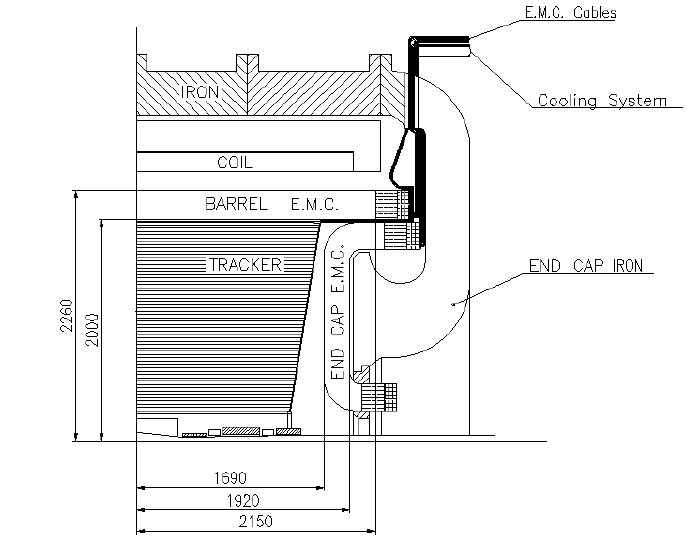
\includegraphics[width=0.8\textwidth]{KLOEsection.png}
	\caption{\label{KLOESection:fig} Cross section of the KLOE detector. The lengths are shown in mm\cite{SAND}.} 
\end{figure}
\subsection{KLOE's electro-magnetic calorimeter}
\label{sec:ECAL}
\begin{figure}
	\centering
	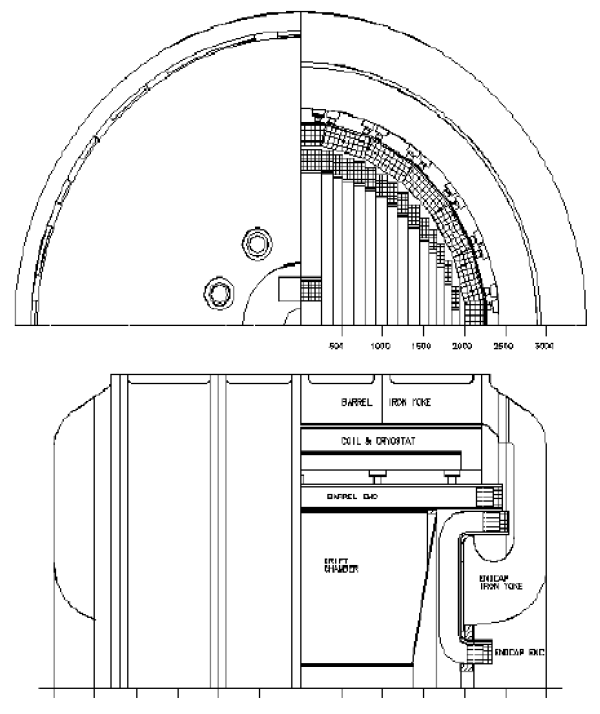
\includegraphics[width=0.8\textwidth]{KLOEECAL.png}
	\caption{\label{KLOEECAL:fig} Schematic cross section of KLOE showing the calorimeters from the front (top figure) and side (bottom figure). The segmentation at the ends of the calorimeters is made to portray the light-guides. The lengths are shown in mm\cite{SAND}.} 
\end{figure}
The KLOE electro-magnetic calorimeter (ECAL) is a sampling calorimeter made of lead and scintillating fiber which offer timing resolution below the ns range, good light transmission and $4\pi$ hermeticity \cite{KLOE magnet}. It will be reused as SAND's calorimeter. The barrel calorimeter is a cylinder segmented into twenty four trapezoidal modules 4.3 m long, 23 cm thick and bases of 52 and 59 cm. The ECAL is completed by two end-caps, divided into vertical modules of variable width and height between 0.7 m and 3.9 m and 23 cm thick. The end-cap modules are bent horizontally to place the photo-tubes in parallel with the magnetic field and ensure the absence of inactive gaps.\\
The modules are read by photo-tubes connecting to photo-guides at both ends of the modules. The read-outs are divided into five planes, the first four being 4.4 cm deep and the last being 5.4 cm deep, each being segmented into 4.4 cm elements.\\
The spacial, energetic and timing resolution evaluations performed during KLOE's commissioning and running phase amount to:
\begin{itemize}
	\item $r-\phi$ or $x-z$ spacial resolution determined by the read-out segmentation: 1.3 cm ($44/\sqrt{12}$ mm)
	\item Energy resolution: $\sigma/E=5\%/\sqrt{E(\text{GeV})}$
	\item Timing resolution: $54/\sqrt{E(\text{GeV})}$ ps
\end{itemize}  
Figure \ref{KLOEECAL:fig} shows the layout of the ECAL with the light read-out segmentation.
\subsection{The inner tracker}
\label{sec: inner tracker}
The inner tracker's design specifications are directly dictated by the necessities of the physics goals of the Near Detector:
\begin{enumerate}
	\item High granularity to guaranty high resolution in momentum, angle and space, maintaining a low density and an overall thickness of about one radiation length $X_0$ to minimize secondary interactions;
	\item Providing a large target for neutrino interactions, with a fiducial mass of the order of $\sim 5 $ tons;
	\item Capability to offer a range of different materials as target;
	\item Particle identification for $e,\pi,K,p,\mu$;
\end{enumerate} 
The first two goals in particular seem to be in contrast with one another requiring at the same time a large target mass and a high precision and low density tracking system.\\
The solution opted by the SAND STT design is to separate the neutrino targets from the tracking system, which are then negligibly light weight with respect to the former. To preserve a low density and achieve the goal of maintaining the detector transparent to secondary particles, the target is spread over the detector in smaller modules. This also makes the goal of having different target materials more easily achievable.
\subsubsection{The straw tube tracker}
One of the two main proposed design now in discussion to achieve the previously detailed goals is a tracker based on low-mass straw tube technology, to be positioned inside KLOE's magnet. The Straw Tube Tracker (STT) would be built in a compact modular fashion, each module being 43.8 mm thick and containing:
\begin{itemize}
	\item Four straw layers disposed in a XXYY configuration. Each straw would be 5 mm in diameter and made of 1000 Angstrom Al coated mylar, containing a tungsten wire 20 $\mu m$ in diameter. These would constitute the tracking component of the detector and would contribute to only 5\% of the total mass, having an average density of $\rho \sim0.17$ g/cm$^3$ and a radiation length of $X_0\sim 2.5$ m;
	\item A polypropylene CH$_2$ solid target slab of 5 mm, whose thickness can be adjusted according to the desired detector mass;
	\item A transition radiation (TR) radiator composed of 150 polypropylene 15 $\mu m$ thick foils, separated by 120 $\mu m$ gaps, occupied by a standard Xe/CO$_2$ 70/30 gas mixture. This specifically optimizes the $e/\pi$ separation;
\end{itemize}  
\begin{figure}
	\centering
	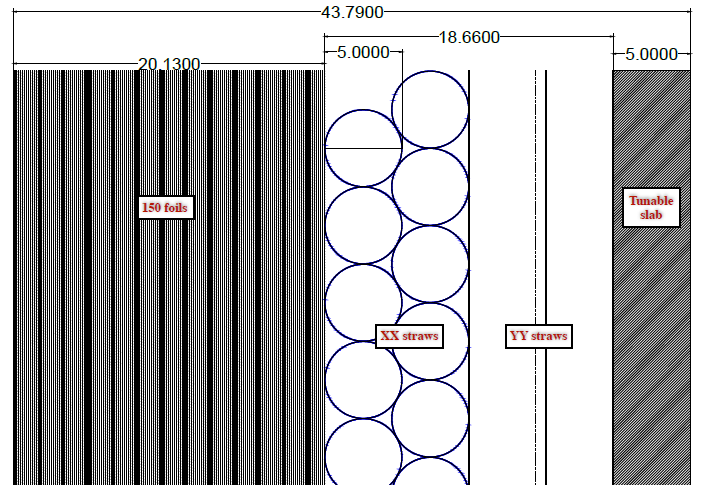
\includegraphics[width=0.7\textwidth]{STTmodule.png}
	\caption{\label{STTmodule:fig} Section of an STT module with its three main components. From left to right: a TR radiator made of 150 foils of polypropylene; four straw tube layers in a XXYY disposition; a CH$_2$ tunable target.} 
\end{figure}
A graphical representation of a section of a STT module is shown in Figure \ref{STTmodule:fig}. Both the polypropylene target and the TR radiator are removable components and can be substituted with a variety of targets. The most important alternative target would be graphite, which is crucial for the measurement of the C background in hydrogen interactions. A 4 mm graphite slab, placed in the same position as the CH$_2$ target slab, would be enough to maintain the same combined $X_0$ of both the polypropylene slab and the radiator. Of the 82 total modules of the STT, the standard CH$_2$ modules would be interleaved with 9 graphite ones, in its standard configuration. This would amount to a total of 677 kg of hydrogen targets and 528 kg of carbon targets.\\
Another important target material is Ca. This could be implemented in the upstream modules much in the same vein as for the graphite. Calcium is important because is isoscalar to Ar allowing a complete characterization of A=40 nuclei, while also enabling various isospin measurements. Many other materials such as Pb and Fe could be implemented, according to the needs of the collaboration. \\
The STT modules support frames need to provide an adequate mechanical support, while also adding a minimal amount of mass. A good compromise can be achieved with a design based on U-shaped beams made of C-composites, so that the $X_0$ traversed by the secondary particles is minimal.\\
The STT design is overall very well equipped to provide for the physics goals set for SAND. It provides a very good spatial ($< 200 \mu m$), angular ($\sim$ 2 mrad), momentum ($\sim 3 \%$) and timing (important for resolving the beam structure) resolutions, while also offering good particle identification by exploiting both the ionization $dE/dx$ and TR for the $e/\pi$ separation. The polypropylene targets, in addition, offer a clean hydrogen target for the neutrino interactions, while also being easily interchanged with other materials at need. An additional small liquid Argon target is also added to the design.
\subsubsection{The liquid Argon meniscus} 
The presence of a small component of liquid Argon in SAND, is essential to understand the nuclear effects of the material that will constitute most of the Far Detector. This meniscus of LAr should be small enough to keep energy loss, showering and multiple Coulomb scattering to a minimum. While the exact position and dimension of this component are still in a phase of optimization, recent designs suggest a volume positioned upstream, almost in direct contact with the ECAL. In the configuration being tested at the moment the meniscus should occupy the first 20 cm of the STT, in a semi-circular shape. Two XXYY straw tube tracker planes are inserted inside the liquid Argon in the meniscus' widest area, just upstream of the STT modules (see Figure \ref{kloe:fig}).
\section{Physics Program}
\subsection{Reducing the systematics}
In order to constrain the systematic uncertainties for the oscillation measurements that DUNE will have to perform, all the variables that enter in eq. \ref{eq:NX} need to be decoupled and measured independently:
\begin{itemize}
	\item $\Phi(E_\nu)$: the flux measurements benefit from low A targets and low density tracker to achieve a high resolution. Both goals are achieved by the STT thanks to the polypropylene targets and the low mass of the straw tubes planes.
	\item $R_{phys}(E_\nu,E_{vis})$: to disentangle the physics response from $R_{det}$ one needs to have in the same detector Ar, H and other light elements targets. The design of the STT modules and the introduction of the LAr meniscus provide all the necessary nuclei.
	\item $\sigma_X(E_\nu)$: once the flux is precisely measured, the cross section on Argon can be evaluated by SAND by using the large sample of interactions provided by the LAr meniscus. Precise cross section measurements require a good characterisation of $R_{phys}R_{det}$ 
	\item $R_{det}(E_\nu, E_{vis})$: the FD detector response factor can be evaluated only by measurements performed in a ND based on liquid Argon technology. The determination of the  $\sigma_{X}R_{phys}$ product, made possible in SAND by the presence of a variety of different nuclear targets, much simplifies the decoupling of $R_{det}$ from the other factors in the eq. \ref{eq:NX}. 
	
\end{itemize}
A detailed characterization of the neutrino fluxes is a necessary condition for all measurements involving the near and far detector, and for the unfolding of the terms in eq. \ref{eq:NX}. SAND will determine both absolute $\nu_\mu$, $\bar{\nu}_\mu $ and relative $\nu_\mu$, $\bar{\nu}_\mu $, $\nu_e$, $\bar{\nu}_e $ fluxes through a series of measurements of different processes, the most important of which are the ones with hydrogen nuclei and electrons.\\
Once the fluxes $\Phi(E_\nu)$ are measured, the other three parameters $\sigma_X R_{phys} R_{det}$ need to be unfolded. The unfolding of $\sigma_XR_{phys}$ requires that both Ar and lighter targets are present in the same detector, so that $R_{det}$ is the same between measurements. In particular for hydrogen targets we have $R_{phys}=1$, which means that the cross-section on H can be accurately measured and the unfolding of the neutrino energy depends only on $R_{det}$ which is defined by $\delta p/p$. Comparing that with interactions on Argon in STT allows for the determination of $\sigma_XR_{phys}$.\\
To constrain $R_{phys}$ separately one can define a set of kinematic variables sensitive to nuclear smearing, and compare the distributions of these observables in CC interaction samples on Ar and H. This strategy allows for a full determination of nuclear smearing effects with the neutrino spectrum seen by the ND, which is different from the one in the FD. For this reason it is essential to measure a complete set of kinematic variables, in order to resolve potential degeneracies.\\
The measurement of $\sigma_X R_{phys}$ and the constraints on $R_{phys}$ offered by SAND can then be compared with the measurements made in the LAr ND ArgonCube to unfold $R_{det}$ in liquid Argon and to validate the predictions for the FD.

\subsection{Precision measurements and new physics}     
The high precision measurements and high statistic sample of the SAND detector and the uniqueness of neutrinos as probes of fundamental interactions allow for an independent physics program of precision measurements and searches for new physics. In this section some of the opportunities presented by this broad physics program are outlined.
\subsubsection{Precision measurements in the electro-weak sector}
The characteristics of SAND allow for an improvement on the previous best measurements of the weak mixing angle ($\sin^2\theta_{W}$), performed by the NuTeV experiment in neutrino DIS interactions \cite{NuTeV}. The measurement of this parameter in SAND would provide a direct determination of the coupling of the neutrinos with $Z^0$ while at the same time probing a different momentum transfer scale than LEP.\\
The DUNE ND complex could measure $sin^2\theta_W$ from the ratio of NC and CC neutrino DIS interactions $\mathcal{R}=\sigma_\nu^{NC}/\sigma_\nu^{CC}$. The high efficiency of the STT  in the determination of electron neutrino CC interactions and in the separation of NC and CC events via kinematic analysis, would allow for a substantial improvement with respect to the previous experiments' systematics and overall precision. The uncertainties in the determination of $\mathcal{R}$ would be dominated by the ones introduced by the theoretical models used for the the structure of the nuclear targets.\\
A separate channel for the determination of the weak mixing angle is the $\nu_\mu e$ NC elastic scattering, which would be uneffected by nuclear model uncertainties, but would be limited in statistics by the small cross section of the process. In particular the observable used would be the ratio between neutrino and antineutrino NC interactions $\mathcal{R}_{\nu e}=\sigma(\bar{\nu}_{\mu}e\rightarrow\bar{\nu}_{\mu}e)/\sigma(\nu_{\mu}e\rightarrow\nu_{\mu}e)$. This measurement is characterized by a totally different momentum transfer scale from the one performed measuring the neutrino DIS interactions. This would allow for a test on the running of $\sin^2\theta_W$.
\subsubsection{Isospin physics tests}
The availability of large statistics of neutrino-hydrogen interactions in SAND allows for the testing of isospin sum rules, which at the moment suffer from low statistics. These include the Adler sum rule $S_{A}= 0.5 \int_{0}^{1}dx/x(F_2^{\bar{\nu}p}-F_2^{\nu p})=I_P$ \cite{Adler}, which gives the isospin of the target and the Gross-Llewyn-Smith(GLS) sum rule $S_{GLS}= 0.5 \int_{0}^{1}dx/x(xF_3^{\bar{\nu}p}-xF_3^{\nu p})$ \cite{GLS}. Both could be measured as a function of the momentum transfer $Q^2$ in neutrino and anti-neutrino interactions on hydrogen from the respective structure functions, which in turn could be determined from the corresponding differential cross-sections. The measurement of $S_A$ in particular would be sensitive to violation of isospin symmetry, charm production and strange sea ($s-\bar{s}$) asymmetries.\\
Thanks to the combination of nuclear and proton (H) targets SAND is also capable of testing isospin charge symmetry (which implies that $F_{2,3}^{\bar{\nu}p}=F_{2,3}^{\nu n}$ and for isoscalar targets $F_{2,3}^{\bar{\nu}}=F_{2,3}^{\nu }$ ).
\subsubsection{Strangeness measurements of the nucleus}
While the strange quark vector elastic form factors have been precisely measured in parity-violating electron scattering experiments, the strange component of the axial-vector form factors $G_{A}^s$ are not yet well determined. SAND will have access to this parameter from measurements of NC elastic scattering off protons $\nu_\mu(\bar{\nu}_\mu)+p\rightarrow\nu_\mu(\bar{\nu}_\mu)+p$. The differential cross section for this process is proportional to the axial vector form factor in the limit that $Q^2\rightarrow0$: 
\begin{equation}
\frac{d\sigma}{dQ^2}\propto G_1^2 = \bigg(-\frac{G_A}{2}+\frac{G_A^s}{2}\bigg)^2
\end{equation}
$G_A$, which is the known axial form factor, can be determined by SAND by measuring the ratio of the NC elastic and quasi-elasti processes over a large $Q^2$ range: $\mathcal{R}_{\nu (\bar{\nu})p}=\sigma(\nu_\mu (\bar{\nu}_\mu)p \rightarrow\nu_\mu (\bar{\nu}_\mu)p)/\sigma(\nu_\mu (\bar{\nu}_\mu)n(p) \rightarrow\mu^-(\mu^+)p(n))$. Note that the determination of $G_A^s$ also represents the most direct method of measuring the value of the nucleon spin $\Delta s$, since for $Q^2=0$ we have that $G_A^s\rightarrow \Delta s$.\\
The space and momentum resolution of the STT also renders SAND capable to do precise measurements of charmed mesons decay modes, such as the $\mu\mu$ and $\mu e$ semi-leptonic charmed decay channels. The study of charm production resulting from $\nu$ and $\bar{\nu}$ interactions with the nuclei, offers a direct probe into the strangeness content of the nucleons \cite{strangeness}.
\subsubsection{Nucleon structure and QCD studies} 
SAND will offer a precise calibration of energy scale uncertainties and high precision measurements of neutrino and antineutrino fluxes. This allows for a determination of nucleon structure functions $F_2,xF_3,F_L,F_T$ using neutrino neutrino and antineutrino DIS interactions. Parton Distribution Functions (PDFs) as well as perturbative and non-perturbative corrections could also be studied performing global QCD analyses over a broad range of $Q^2$ and Bjorken x. The presence of both Hydrogen and nuclear targets in SAND are essential to separate valence and sea quarks distributions, $d$ and $u$ distributions as well as $s$ and $\bar s$ distributions.  
\subsubsection{Neutrino-nucleus interaction studies} 
The modular structure of STT allows for the integration of many different nuclear target. This creates the possibility of studying how the nucleon structure is modified inside a heavy nucleus, by measuring structure functions, form factors and cross-sections. The study of final state interactions is also important, since they can introduce a significant smearing in the reconstruction of the kinematics variables of the final state particles. 
\subsubsection{New physics searches}
All the precision measurements described in the present are potentially sensitive to many BSM (Beyond the Standard Model) effects which would manifest as deviations from the SM predictions. Sand is also capable of more direct searches for new physics. One possible field of study would the test of the MiniBooNE low energy anomaly at different but similar $L/E$. SAND would be particularly well set for the task thanks to the electron identification capability and high resolution of STT.\\
The oscillation into sterile neutrino explanation for the MiniBooNE anomaly could be tested by measuring the CC ratios for both neutrinos and antineutrinos $\mathcal{R}_{e\mu}=(\nu_e N \rightarrow e^-X)/(\nu_\mu N \rightarrow \mu^- X)$ and $\bar{\mathcal{R}}_{e\mu}=(\bar{\nu}_e N \rightarrow e^+ X)/(\bar{\nu}_\mu N \rightarrow \mu^+ X)$ as well as the NC/CC ratio $\mathcal{R}_{\nu(\bar{\nu})p}$ as a function of $L/E$. These measurements would be sensitive to both appearance and disappearance anomalies in all four neutrino spectra. STT would also be sensitive to $\nu_\tau$ appearance, which could result from both sterile neutrino oscillations or BSM interactions.\\
SAND would also enhance the sensitivity of the ND to dark sector physics. This includes heavy sterile neutrino searches ( of the type proposed in the see-saw mechanism ), axions, dark photons, WIMPs and many others.


 
\chapter{The simulation}
\rhead[\fancyplain{}{\bfseries Chapter 4: The simulation}]{\fancyplain{}{\bfseries\thepage}}
\lhead[\fancyplain{}{\bfseries\thepage}]{\fancyplain{}{\bfseries Chapter 4: The simulation}}
          \label{chapter 4}
The simulation performed for this thesis required the utilisation of a few different software, all selected following the ND collaboration recommendations \cite{ND collaboration}. In order to simulate the neutrino interactions with matter we used the neutrino event generator GENIE, which has been officially adopted by the DUNE collaboration (Section \ref{sec: GENIE}). The geometry of SAND and the Near Detector complex were produced in form of GDML files, using $dunendggd$, a geometry generation tool entirely based on GGD (General Geometry Description). The present SAND's ECAL geometry in particular has been produced during this thesis (Section \ref{sec: GGD}). The propagation of the particles generated by the neutrino interactions in the geometry was done using edep-sim, a simulation tool based on Geant4 (Section \ref{sec: edep-sim}). Finally the digitization and reconstruction of the signal produced in the ECAL and STT was done using C++ code, based on previous simulations performed for the KLOE detector (Sections \ref{sec: digitization} and \ref{sec: Reconstruction}).    
\section{GENIE: MC neutrino generator}
\label{sec: GENIE}
GENIE is a ROOT-based neutrino Monte Carlo (MC) generator, designed using object-oriented methodologies and developed in C++ \cite{GENIE manual}. The present version provides comprehensive neutrino interaction modelling in a range that spans from about 100 MeV to a few hundred GeV, with the long term goal of expanding down to around 1 MeV and up to $\sim 1$ PeV. \\
GENIE has been adopted by the majority of neutrino experiment, and is the first attempt at a canonical neutrino event generator. Such a tool is essential in the design and execution of the new generation of neutrino experiments, including DUNE, that aim to reach new levels of precision. The universality of GENIE in the neutrino experimental field, in particular, solves many problems that the previous MC generator had, due to the fact that they were developed independently for each experiment (for example GENEVE, NEUT, NeuGEN). This limitation made the generators fragile and in many cases incapable of keeping up with the state of the art in terms of theoretical models and experimental data.\\
GENIE also responds to the necessity of having consistent modelling over the wide energetic range of interest for present and future neutrino experiments, where perturbative and non-perturbative nucleon interactions and many scattering mechanisms are relevant. Often cross section, hadronization and nuclear models have different ranges of validity and need to be pieced together in order to cover all of the available phase space. There are also cases outside these ranges of validity for which new models need to be developed with the additional problem of the general lack of data in the ranges of modern accelerator neutrino experiments. In many cases the simulations are still tuned using data from bubble chamber experiments that date back to the 70's and 80's.
\subsection{GENIE usage for the ND collaboration}
GENIE takes as input a neutrino flux and a geometry representation, and gives as output a file with information regarding the process simulated and the particles in the final state. In particular the output file contains the list of particles that exit the struck nucleus after scattering interaction, hadronization and final state interactions. This file is then handed to edep-sim for propagation through the detector geometry.\\
The fluxes files used by the ND group and in the scope of this thesis are taken from the LBNF beam simulation under the guidance of the beam group. These files come in a variety of formats such as: 
\begin{itemize}
	\item \emph{dk2nu} files which record information about the decay of hadrons and muons that generate the neutrinos in the beam line, while also providing a flux driver to integrate into GENIE;
	\item \emph{GSimpleNtpFlux} files, a NTuple format contained into GENIE for storing flux ray information with minimal formatting;
	\item \emph{ROOT histograms} containing informations regarding the flux neutrino spectrum for all flavours, at the ND (before oscillation) and FD (after oscillation) and the respective CC and NC event rates as a function of energy;
\end{itemize}  
For the simulation performed in this thesis the latter format has been used. In particular the files are the ones produced with the optimized 3-Horn Design by the LBNF group and presented in the Beam Optimization Review of October 2017 \cite{flussi}. The un-oscillated neutrino and antineutrino spectra and NC/CC interaction rates are shown in Fig \ref{NuFlux:fig} and Fig. \ref{NubarFlux:fig} respectively for the FHC configuration.\\
Note that the calculation of cross sections for individual sub-processes are pre-calculated as a function of neutrino energy and stored in XML formatted splines. The ones used in this thesis have been partially retrieved from the previously existing ones recommended by the ND collaboration and partially generated using GENIE's internal spline generator. 
\clearpage
\begin{figure}
	\centering
	\begin{subfigure}[b]{0.475\textwidth}
		\includegraphics[width=\textwidth]{NuFlux.png}
		\caption{}
	\end{subfigure}
	\hfill
	\begin{subfigure}[b]{0.475\textwidth}
		\includegraphics[width=\textwidth]{NuEventRates.png}
		\caption{}
	\end{subfigure}
	\caption{\label{NuFlux:fig}Simulation histograms for the neutrino flux produced with the optimized 3-Horn Design by the LBNF collaboration and presented in the Beam Optimization Review of October 2017: (a) Muon and electron neutrino logarithmic fluxes as a function of energy (GeV) in units of $\nu s/m^2/\text{POT}/GeV$.  (b) Muon and electron neutrino CC and NC logarithmic event rates as a function of energy (GeV) in units of events/kton/POT/GeV \cite{flussi}. } 
\end{figure}
\begin{figure}
	\centering
	\begin{subfigure}[b]{0.475\textwidth}
		\includegraphics[width=\textwidth]{NuBarFlux.png}
		\caption{}
	\end{subfigure}
	\hfill
	\begin{subfigure}[b]{0.475\textwidth}
		\includegraphics[width=\textwidth]{NuBarEventRates.png}
		\caption{}
	\end{subfigure}
	\caption{\label{NubarFlux:fig} Simulation histograms for the anti-neutrino flux produced with the optimized 3-Horn Design by the LBNF collaboration and presented in the Beam Optimization Review of October 2017: (a) Muon and electron anti-neutrino logarithmic fluxes as a function of energy (GeV) in units of $\nu s/m^2/\text{POT}/GeV$.  (b) Muon and electron anti-neutrino CC and NC logarithmic event rates as a function of energy (GeV) in units of events/kton/POT/GeV \cite{flussi}. } 
\end{figure}
\clearpage
\section{GGD: geometry generation tool }
\label{sec: GGD}
\begin{figure}
	\centering
	\includegraphics[width=0.9\textwidth]{hall.png}
	\caption{\label{hall:fig} Image of the ND hall geometry generated with \emph{dunendggd} and drawn using the OGL ROOT graphic tool.} 
\end{figure}
The General Geometry Description (GGD) is a python based software system used to generate GDML files containing descriptions of constructive solid geometries \cite{ggd}. The geometry conventions are the ones used by ROOT and Geant4. \\
The DUNE ND collaboration has developed its own geometry generation tool called \emph{duneggdnd}, entirely based on GGD \cite{dunendggd}. In Fig. \ref{hall:fig} an image of the ND hall geometry generated with \emph{dunendggd} and drawn using the OGL ROOT graphic tool is shown. It contains the LAr detector ArgonCube, HPgTPC and SAND. The origin of coordinates is chosen to be the location where the beam enters the hall which is assumed to be 574m from the beam's origin, directly on the beam axis.\\
 \begin{figure}
	\centering
	\begin{subfigure}[b]{0.8\textwidth}
		\includegraphics[width=\textwidth]{kloelat.png}
		\caption{}
	\end{subfigure}
	\hfill
	\begin{subfigure}[b]{0.8\textwidth}
		\includegraphics[width=\textwidth]{kloefront.png}
		\caption{}
	\end{subfigure}
	\caption{\label{kloe:fig} Front (a) and lateral (b) cross section of the SAND geometry produced with \emph{dunendggd} and drawn with the ROOT graphical tool OGL. The main components of the detector are highlighted: the iron yoke, the magnet, the ECAL, the STT and the LAr meniscus.} 
\end{figure}
SAND's geometry descriptions have been produced by the Near Detector collaboration, both for the STT configuration described in Chapter 3 and for its alternatives. A graphical representation of the STT design developed with \emph{dunendggd} is shown in Figure \ref{kloe:fig}, with its main components highlighted: the iron yoke, the magnet, the ECAL, the STT and the LAr meniscus. The final design are in a phase of development and tuning, making new tweaks to the geometries a frequent occurrence. The present geometries for the two active components of the detector (i.e. the ECAL and the STT) will be described more in detail in this section.
\subsection{SAND's ECAL: geometry}
\begin{figure}
	\centering
	\includegraphics[width=0.7\textwidth]{ecal.png}
	\caption{\label{ecal:fig} SAND's ECAL's geometry generated with \emph{dunendggd} and drawn using the OGL ROOT graphic tool. The distance between the two inner faces of the end-caps (338 cm) and the length of the barrel section (430 cm) are highlighted.} 
\end{figure}
For the purposes of this thesis, a new geometry for SAND's electro-magnetic calorimeter has been produced. As described in Section \ref{sec:ECAL} SAND's ECAL is a sampling calorimeter made of lead and scintillating fibre divided into a barrel section and two end-cap sections. The barrel calorimeter is a cylinder segmented into twenty-four trapezoidal modules 4.3 m long, 23 cm thick and bases of 52 and 59 cm. The two end-caps are divided into forty-five vertical modules of variable width and height. \\
A series of approximations, based on previous Fortran simulations made for the KLOE detector, have been made in the geometry. The calorimeter modules have been constructed from alternating slabs of plastic scintillator and lead, rather than from individual fibres. Both the end-cap and barrel modules are composed of 209 slabs of each kind, the Pb slabs being 0.04 cm thick and the scintillating ones being 0.07 cm thick.\\
The second simplification consists in the fact that, while the barrel modules are simulated with their real dimensions and shape, the end-caps are approximated to be two hollow cylinders of inner diameter 41.6 cm and outer diameter 400 cm. The ``bend" that characterises the real end-cap is not reproduced, and no further separation into modules is simulated. The end-cap segmentation, as well as the simulation of the individual read-out cells is left to the digitisation step of the simulation.\\
In Figure \ref{ecal:fig} a graphical representation of the entire calorimeter is shown, while the individual barrel and end-cap modules are shown in Figure \ref{calmod:fig}.
\begin{figure}
 	\centering
 	\begin{subfigure}[b]{0.9\textwidth}
 		\includegraphics[width=\textwidth]{ECALmodule.png}
 		\caption{}
 	\end{subfigure}
 	\hfill
 	\begin{subfigure}[b]{0.8\textwidth}
 		\includegraphics[width=\textwidth]{endcapECAL.png}
 		\caption{}
 	\end{subfigure}
 	\caption{\label{calmod:fig} Front and lateral cross section of a ECAL barrel module (a) and a ECAL endcap module (b). The geometries have been produced with \emph{dunendggd} and drawn with the ROOT graphical tool OGL. The components in green represent the scintillator slabs, while the the components in grey represent the Lead slabs.} 
\end{figure}
\subsection{SAND's STT: geometry}
The Straw Tube Tracker is currently in a design stage and its configuration is subject to frequent modifications. In this section we describe the geometry used in the simulations performed during this thesis.\\
The STT is composed by 3 different modular components:
\begin{itemize}
	\item The standard polypropylene modules, composed of a C$_3$H$_6$ target slab, a XXYY straw tube tracking plane and a 150 foils TR radiator;
	\item The graphite modules composed of a C target slab and  a XXYY straw tube tracking plane;
	\item The slab-less modules, which do not offer any target slab and only include the straw tubes planes and the TR radiator; 
\end{itemize}
The Liquid Argon meniscus, complemented by two straw tube XXYY planes placed on the contact surface between the LAr and the STT modules, completes the composition of SAND's inner tracking region.\\ 
The dimensions and composition of the modules' internal elements are coherent with the ones reported in Section \ref{sec: inner tracker}, with the only omitted components being the support structures.\\
The STT is composed of 90 total modules plus the LAr meniscus, which is positioned at the front of the detector. Proceeding downstream the first 85 modules are alternated between the 78 polypropylene ones and the 7 graphite ones. Specifically, after the first three modules, which are polypropylene, the graphite modules are one every thirteen. The last 5 modules are slab-less.\\ 
While the thickness of the modules are consistent throughout the tracker region, their $xy$ plane area varies so that the corners always touch the internal walls of the calorimeter modules and the smallest possible amount of empty space is left.
\clearpage
\section{Edep-sim: charged particle propagation}
\label{sec: edep-sim}
\begin{figure}
	\centering
	\includegraphics[width=0.9\textwidth]{viewer.png}
	\caption{\label{viewer:fig} Image of a $\nu_\mu$ CC interaction generated in SAND's ECAL's geometry with GENIE and propagated using edep-sim. The green dots represent the energy deposition hits of the exiting muon. The image has been produced using edep-sim's internal viewer: edep-disp.} 
\end{figure}
The energy deposition simulation (edep-sim) is a wrapper around the GEANT4 particle propagation simulation \cite{edep-sim}. Given a particle kinematics input file and a GDML or ROOT geometry file, edep-sim is capable of simulating the particles' propagation.\\
Edep-sim supports a variety input file formats, including both NEUT and GENIE output files. In particular GENIE files are read in the ``rootracker" format, which is a GENIE event ROOT tree standard evolved from work performed with the purpose of integrating the GENIE simulations with the nd280, INGRID and 2km detector-level MC generators. In particular during this thesis the t2k variant of the format was used. \\
Edep-sim is also capable of generating and propagating beams of particles in a more standard way using Geant4 command macros. This capability was also used in the scope of this thesis.\\
The edep-sim output is a standard ROOT file containing two keys: a TGeoManager object with the simulated  geometry, and a TG4Event tree (an edep-sim specific class) containing the event information. The TG4Event class contains the event number, the run number, information about the propagated primary particles, the particle tracks and the energy deposition.\\
In Figure \ref{viewer:fig} a graphical representation of a neutrino event generated using GENIE and propagated using edep-sim in SAND's simulated geometry is shown. It is a $\nu_\mu$ CC interaction, generated in one of SAND's ECAL front modules. The figure was produced using edep-disp, edep-sim's internal event viewer.
\section{Signal digitization}
\label{sec: digitization}
For signal digitization we mean the simulation of the signal production in the read-out systems of the detector, in accordance with the energy deposition of the particles. In the ECAL this implies the segmentation of the calorimeter modules into cells and the simulation of the photo-electron production in the photo-multiplier tubes. In the STT it requires assigning the hits and their energy deposition to the correct straw tube. 
\begin{figure}
	\centering
	\includegraphics[width=0.9\textwidth]{cellbarrel.png}
	\caption{\label{cellbarrel:fig} Graphical representation of the segmentation of one of the barrel calorimeter modules. The module is divided into five vertical layers: the first four from the bottom are 4.4 cm thick and the last is 5.4 cm thick. Each layer is further divided into 12 horizontal cells. } 
\end{figure}
\subsection{SAND's ECAL: digitization}
The photo-electrons produced in the ECAL fibres by passing charged particles, are collected by photo-multiplier tubes connected at both ends of the calorimeter modules. These PMs define a segmentation in the signal collection into layers and cells. We simulate this division via a signal digitization C++ program that takes the information contained in the edep-sim output trees and, given the position of the hits, assigns the energy deposition to the correct calorimeter cell. The program has been developed based on previous simulations performed by the KLOE collaboration, and adapted during the scope of this thesis to the new geometry.\\
The barrel calorimeter modules are divided into five horizontal layers. Starting from the smaller base, layers number 0 to 3 contain 40 Pb slabs and 40 scintillator slabs each, for a total of 4.4 cm in thickness. Layer 4 is 5.4 cm thick, containing 49 slabs of each kind. The layers are further divided into 12 trapezoidal cells, each having equally large bases. The cells are numbered from left to right as shown in Figure \ref{cellbarrel:fig}. Each module is also assigned a number id from 0 to 23, starting from the top module and proceeding clockwise with respects to the positive $x$ axis.\\
The two end-cap modules are similarly divided into four layers having the same thicknesses of the barrel modules' ones. Each layers contains 45 rectangular cells all having the same area. The enumeration of the cells and layers is analogous to the one for the barrel modules, while the two end-caps are given the id's 30 and 40.\\
\begin{figure}[t!]
	\centering
	\includegraphics[width=\textwidth]{showevent.png}
	\caption{\label{showevent:fig} Graphical representation of the digitized signal produced by the particles generated in a $\nu_\mu$ CC interaction event, having vertex in one of the front calorimeter modules. The cells hit by the particles are coloured in red and black. The particle tracks are also highlighted, with the muon being coloured in blue, the neutrons in grey and the electron in red. The left panel presents a projection on the $zy$ plane and the right one on the $xy$ plane ($z$ being the horizontal projection of the neutrino beam direction and $y$ being the vertical axis). Both are scaled according to the global ND hall coordinates.  } 
\end{figure}
Once the calorimeter is properly segmented we extract the information contained in the edep-sim output files, regarding the hits of the propagated particles contained in the active scintillator slabs. Each hit is automatically assigned by edep-sim to the module in which the slab is contained. Given the hit position we then allocate it in the correct.\\ 
Proceeding this way for each simulated event, each cell is assigned a collection of hits, each being associated to a certain time and energy deposition. An attenuation factor is applied to each hit energy deposition to take into account the fibres' attenuation:
\begin{equation}
	E_{A}= p_1 \times \exp\bigg(-\frac{d}{alt1}\bigg)+ (1-p_1)\times \exp\bigg(-\frac{d}{alt2}\bigg)
\end{equation}
where $d$ is the distance between the hit and the photo-cathode, $p_1=0.35$, $alt1=50$ cm and $alt2$ is 430 cm for planes 0 and 1, 380 cm for plane 2 and 330 cm for planes 3 and 4. For each MeV of energy after the attenuation factor is applied on average 25 photo-electrons are produced. The number of p.e. for each hit is then extracted from a Poisson distribution having $25 \times E_A \times dE$ as its most probable value. The ADC (analogue to digital converter) signal assigned to the PM for each event is proportional to the total number of photo-electrons produced on the photo-cathode. In our simple simulation the two numbers coincide.\\ 
A graphical representation of the energy deposition divided between the calorimeter cells is shown in Figure \ref{showevent:fig}. The event displayed is the same as the one shown in Figure \ref{viewer:fig}.\\
To each photo-electron is also assigned an arrival time on the PMT. This is simulated as being obtained via time to digital converters (TDC) applied to the PMs at both ends of the cells. Each cell is thus associated with two time values from the TDC's: $t_{TDC1}$ and  $t_{TDC1}$. The individual photo-electron time $t_{p.e.}$ is given by:
\begin{equation}
t_{p.e}= t_{part}+ t_{decay}+ d \cdot u_{ph} + Gauss(\text{1ns}) 
\end{equation}
where $t_{part}$ is the time associated to the passage of the particle through the scintillating material, $t_{scint}$ is the scintillation decay time, $d$ is the distance between the hit and the PM, $u_{ph}=5.85$ ns/m is the inverse of the propagation velocity of the photons in the scintillator material (and thus $d \cdot u_{ph}$ is the photon propagation time) and $Gauss$(1ns) is the uncertainty, extracted from a Gauss distribution with the most probable value being 1 ns. \\
The scintillation decay time is given by:
\begin{equation}
t_{decay}=t_{scin}\cdot\bigg(\frac{1}{r_{ph}(1)}-1\bigg)^ {t_{scex}}
\end{equation}
where $t_{scin}=3.08$ ns and $t_{scex}= 0.588$ . Each photo-electron is thus assigned a time $t_{p.e}$, producing two time arrays on the PM. The two TDC times $t_{TDC1}$ and $t_{TDC2}$, are given by selecting the p.e. time that is positioned at 15\% of the $t_{p.e.}$ ordered list for each of the two TDC's constant fraction.\\
At the end of the digitization process, an output file is produced, in which for each event, for every cell in which there was an energy deposition, the following information is recorded:
\begin{itemize}
	\item The spatial position of the cell centre in the global coordinates of the ND hall;
	\item The module, layer and cell identification numbers and the module length;
	\item The two ADC values, corresponding to the number of photo-electrons produced on each photo-cathode ($N_{p.e.1}$ and $N_{p.e.2}$);
	\item The two TDC times ($t_{TDC1}$ and $t_{TDC2}$); 
	\item Two arrays containing the photo-electron times in increasing order ($t_{p.e.1}[N_{p.e.1}]$ and $t_{p.e.2}[N_{p.e.2}]$) ;
	\item Two index arrays linking the p.e. times to the hits that produced them stored in the Monte Carlo truth edep-sim file;
\end{itemize}
\subsection{SAND's STT: digitization}
The active component of the STT modules consists of two double layers of straw tube trackers: the first placed horizontally (XX) and the second placed vertically (YY). The first step of the digitization of these detector components, consists in dividing the hits produced by the particles propagated using edep-sim, into clusters: one for each straw contained in the detector. The hits are then reorganised from the first to the last being produced in each straw. Finally an output file is generated, where for each straw hit by at least one particle, the following information is contained:
\begin{itemize}
	\item The straw name, in which the module and the plane are specified;
	\item The $x$, $y$, and $z$ in the ND hall coordinate system and the time associated to the hit cluster. Each of the coordinates is calculated simply as the mean between the value associated to first and last hits in the cluster;
	\item The total energy deposition of the hit cluster;
	\item A flag indicating if the straw hit is horizontal or vertical;
	\item A index array mapping the cluster to the hits that produced it from the Monte Carlo truth;
\end{itemize}
\section{Reconstruction}
\label{sec: Reconstruction}	
The reconstruction C++ code is divided between the track reconstruction performed in the STT and the cluster reconstruction in the ECAL. The first performs a fit of the helicoidal trajectory described by the charged particles moving in the STT magnetic field. It does so using the hit coordinate information from the STT digitization output, which also allows for a reconstruction of the particle initial momentum. The second reconstructs the energy deposition in the calorimeter from the digitized cell signal.
\subsection{SAND's ECAL: cluster reconstruction}
The information from the digitized signal produced in the calorimeter, is used to group the cells with energy deposition into cluster, each associated to a specific particle track. In order to do so we first find for each cell, the particle that produced the most p.e., using the track id. from the Monte Carlo truth. For each track that produced the largest amount of p.e. in at least one cell, we create a collection of cells, or cluster, containing each cell in which the particle had the largest energy deposition.\\
For each cell in the cluster we evaluate the position of where the particle hit it and when. In the ND hall coordinates the $z$ is always taken as the centre of the cell. For the barrel ECAL modules, which are placed horizontally, the $y$ coordinate is also estimated this way, while the $x$ is evaluated using the information from the cell TDC's:  
\begin{equation}
\label{eq: cell x}
x=\frac{t_{TDC1}-t_{TDC2}}{2u_{p.e.}}+x_{cell}
\end{equation}
where $x_{cell}$ is the coordinate of the cell centre, while $t_{TDC1}$, $t_{TDC1}$ and $u_{p.e.}$ are the same quantities defined in Section \ref{sec: digitization}. For the end-cap cells, which are placed vertically the opposite is true: the $x$ is taken as the cell centre, while the $y$ is calculated as in Eq. \ref{eq: cell x}. The time value for each cell is calculated by taking the mean from the two TDC value and subtracting the maximum photon propagation time:
\begin{equation}
t=\frac{1}{2}(t_{TDC_1}+t_{TDC2}-u_{p.e.}\times L)
\end{equation} 
where $L$ is the total length of the cell.\\
For each cluster a weighted average of the coordinates $(x_{cl},y_{cl},z_{cl},t_{cl})$ is calculated, using the total energy deposition for each cell $E_{cell}$ as weights. These values are given in the output file together with the total energy deposition $E_{cl}$ and the variance.\\
The average  $(x,y,z,t)$ is also calculated for each calorimeter layer in the cluster. These values are then used to perform linear fits on the $zx$ and $zy$ planes in order to estimate the components of the direction versor of the particle trajectory in the calorimeter. Whether the particle is entering or escaping the detector is evaluated by calculating:
\begin{equation}
d=\frac{(z_{out} - z_{in})(t_{out} - t_{in})}{|(z_{out} - z_{in})(t_{out} - t_{in})|}=\pm1
\end{equation} 
where $z_{out}$ and $z_{in}$ are the $z$ coordinates for the most outer and most inner layer hit in the cluster, respectively (analogously for $t_{out}$ and $t_{in}$). The particle is escaping if $d=+1$ and entering if $d=-1$. 
\subsection{SAND's STT: track reconstruction}
\label{sec: track reconstruction}
A charged particle entering the tracking region of the SAND detector is effected by the 0.6 T magnetic field $\vec{B}$, pointing in the $x$ direction of the ND hall coordinates. It thus describes a helical trajectory: a combination of the circular motion on $zy$ plane, perpendicular to the magnetic field and a linear motion parallel to $B$ in the x direction (Figure \ref{helix:fig}). The helix can be described parametrically as a function of the spatial progression along the trajectory $s$ \cite{tracking}:
\begin{equation}
\begin{cases}
	z(s)=z_0+R\Big(\cos(\Phi_0+\frac{hs\cos\lambda}{R})-\cos\Phi_0\Big)\\
	y(s)=y_0+R\Big(\sin(\Phi_0+\frac{hs\cos\lambda}{R})-\sin\Phi_0\Big)\\
	x(s)=x_0+s\sin\lambda
\end{cases}
\end{equation} 
where $(x_0,y_0,z_0)$ is arbitrary and can be taken as the coordinates of the first point along the trajectory, $\Phi_0$ is the angle between the $z$ axis and the segment connecting the centre of the circumference $(y_C,z_C)$ and the point $(y_0,z_0)$ in the $yz$ plane, $R$ is the radius of the circumference, $\lambda$ is the angle between the initial velocity vector $\vec{v}$ and the plane perpendicular to $\vec{B}$ known as the dip-angle and finally $h=\pm1$ is the sense of rotation on the helix.\\
The projection of the trajectory on the $yz$ place thus describes a circle:
\begin{align}
(z-z_0+R\cos\Phi_0)^2+(y-y_0+R\cos\Phi_0)^2&=\\
(z-z_c)^2+(y-y_c)^2&=R^2
\end{align}
Performing a circular fit on the hits recorded in the horizontal straws, on the $yz$ plane, we can get the most probable values for $R$ and $(y_C,z_C)$ for each particle trajectory.\\
\begin{figure}
	\centering
	\begin{subfigure}[b]{0.475\textwidth}
		\includegraphics[width=\textwidth]{helicoidal.png}
		\caption{}
	\end{subfigure}
	\hfill
	\begin{subfigure}[b]{0.475\textwidth}
		\includegraphics[width=\textwidth]{circular.png}
		\caption{}
	\end{subfigure}
	\caption{\label{helix:fig}(a) Helicoidal motion of a charged particle in the magnetic field $\vec{B}$ which in the STT is parallel to the $x$ axis in the ND hall (b) Projection of the helicoidal motion on the $yz$ plane \cite{tracking}.} 
\end{figure}
We would now like, in order to have a complete description of the particle motion, to perform a reconstruction on the dip-angle $\lambda$. In order to do so we first approximate the circular motion in the $yz$ plane to a parabolic motion by applying a first order Taylor expansion in $s/R$. This is justified if $s/R\ll1$, and thus if the portion of the circular trajectory described by the particle is small with respects to $R$; this is true for the energetic muons entering SAND. We also switch from $\Phi_0$ to the angular direction of the track in $(x_0,y_0,z_0)$ which we indicate as $\varphi_0=\pi/2-\Phi_0$. Finally we write $(y_0,z_0)$ as $y_0=d_0\cos\varphi_0$ and $z_0=-d_0\sin\varphi_0$, where $d_0$ is simply the distance between the initial point and the origin of coordinates in the $yz$ plane. The equations of motion then become:
\begin{equation}
\begin{cases}
z(s)=-d_0\sin\varphi_0+s\cos\lambda\cos\varphi_0+\frac{h}{2R}s^2\cos^2\lambda\sin\varphi_0\\
y(s)=d_0\cos\varphi_0+s\cos\lambda\sin\varphi_0-\frac{h}{2R}s^2\cos^2\lambda\cos\varphi_0\\
x(s)=x_0+s\sin\lambda
\end{cases}
\end{equation}   
We can now perform a coordinate rotation in the $yz$ plane of an angle $\varphi_0$, so that the new $z$ axis, which we will call $\rho$, is directed along the track trajectory in $(x_0,y_0,z_0)$ :
\begin{align}
\rho &=z\cos\varphi_0+y\sin\varphi_0\\
y'&=-z\sin\varphi_0+y\cos\varphi_0
\end{align}
The equations of motion can now be re-written to be divided between the plane $y'\rho$ and the plane $\rho x$:
\begin{equation}
\begin{cases}
x=x_0+\rho\tan\lambda\\
y'=d_0-\frac{h}{2R}\rho^2 
\end{cases}
\end{equation}
From the first equation we can see that performing a linear fit on the transverse plane gives us the values of $\tan(\lambda)$ and $z_0$. In order to do so we use the information from the trajectory hits in the vertical straws, which give us the x and z coordinates. The y values are extrapolated using the $R$ and $(y_C,z_C)$ from the circular fit:
\begin{equation}
y= y_C + h\sqrt{R^2-(z-z_C)^2}
\end{equation} 
The value of $h=\pm1$ (+1 is clockwise, while -1 is counter-clockwise), is given accordingly by the sign of the product of the z distance between the first and second hit of the track and the y distance between $y_C$ and $y_0$: 
\begin{equation}
h=\frac{(z_1-z_0)(y_C-y_0)}{|(z_1-z_0)(y_C-y_0)|}=\pm1
\end{equation}
In order to calculate $\rho$ we also need the values of $\cos\varphi_0$ and $\sin\varphi_0$. We can calculate them as:
\begin{align}
\cos\varphi_0&=h(y_0-y_c)/R\\
\sin\varphi_0&=-h(z_0-z_c)/R
\end{align} 
If both fits were successful we now have estimates for $R$, $(y_C,z_C)$ and $\lambda$. With this information we can reconstruct the initial transverse momentum of the particle on the $yz$ plane using the formula:
\begin{equation}
p_T\text{ [GeV]}=0.3\times B\text{ [T]}R\text{ [m]}
\end{equation}
We can then get the three components of the momentum in the ND hall coordinate system as:
\begin{equation}
\begin{cases}
p_z=p_T\cos\varphi_0\\
p_y=p_T\sin\varphi_0\\
p_x=p_T\tan\lambda 
\end{cases}
\end{equation}
Having the three momentum components we can then reconstruct the total momentum module, which in case of relativistic particles is about the same as the particle energy:
\begin{equation}
E_{reco}\simeq p_{reco} = \sqrt{p_x^2+p_y^2+p_z^2}
\end{equation}


\chapter{Beam monitoring: analysis and results}
\rhead[\fancyplain{}{\bfseries Chapter 5: Beam monitoring: analysis and results }]{\fancyplain{}{\bfseries\thepage}}
\lhead[\fancyplain{}{\bfseries\thepage}]{\fancyplain{}{\bfseries Chapter 5: Beam monitoring: analysis and results}}
\label{chapter 5}
\section{Overview}
Since new measurements in the neutrino sector need a high precision knowledge of the neutrino flux produced by the new high intensity beam facility, beam monitoring is  essential. Many observables can be used for beam monitoring. In this study we have considered the reconstructed momenta of muons produced in $\nu_\mu$ CC interactions in SAND's front electro-magnetic calorimeter modules. The shape of the reconstructed momentum spectrum of the muons produced in CC interactions, depends on the original $\nu_\mu$ energy spectrum. Any anomalies in the beam production would thus in principle cause variations in both spectra. In particular we considered the anomalies generated when the first neutrino beam horn experienced a transverse displacement of +0.5 mm in the $y$ coordinate\\
Neutrino interactions samples were simulated using the GENIE neutrino Monte Carlo generator forcing the interaction vertexes to be in one of the nine frontal barrel calorimeter modules (Figure \ref{front:fig}). The particles produced in the interactions were then propagated with edep-sim, the ECAL and STT signals were digitized and the clusters and tracks reconstructed. Note that in order to shorten the simulation times the digitization and reconstruction steps were performed only on the primary particles of the interactions.\\
No particle identification has been implemented for SAND's simulation chain at the time of writing. The muon tracks where thus selected from the Monte Carlo truth PDG code informations. In order to reject the background coming from particles outside KLOE and then passing through the calorimeter (not simulated in this work), a selection on the energy deposition on the most outer layer of the ECAL was implemented. This energy deposition threshold, together with a selection on the $x$ position of the neutrino vertexes defined our fiducial cut. \\
Only the successfully reconstructed muons were considered. Additionally the $\chi^2$ values for the linear and circular fits were used to identify a reconstruction quality selection. \\
We studied the sensitivity to the beam modification by applying two-sample homogeneity tests on the reconstructed muon momentum distributions. We used samples roughly corresponding to the amount of CC interactions expected in the front calorimeters of SAND in a week, as suggested by the ND collaboration for beam monitoring measures. Given the CC interaction event rate $r_{CC}=4.685\times 10^{5}\ \text{ev}[\nu_{\mu}(CC)]/$ton/week, the module mass $m_{mod}=2.75$ ton, the number of target modules $n_{mod}=9$ and the fraction of CC events with respects to the total $f_{CC}=2/3$ this corresponds to:
\begin{equation}
N_{week}=r_{CC}\times f_{CC}^{-1} \times m_{mod} \times n_{mod}\simeq 1.74\times 10^6
\end{equation} 
We thus produced a ``nominal" (standard neutrino beam energy distribution) and a ``shifted" (neutrino beam produced with +0.5 mm $y$ shift in the first horn) sample both containing exactly $N=1750000$ neutrino interactions.
\begin{figure}[t]
	\centering
	\begin{subfigure}[b]{0.55\textwidth}
		\includegraphics[width=\textwidth]{frontcaloXY.png}
		\caption{}
	\end{subfigure}
	\hfill
	\begin{subfigure}[b]{0.4\textwidth}
		\includegraphics[width=\textwidth]{frontcaloYZ.png}
		\caption{}
	\end{subfigure}
	\caption{\label{front:fig} Graphical representation (produced with OGL) of the 9 front calorimeter barrel modules GEANT4 geometries. The two panels show the projection (a) on the $xy$ plane and (b) on the $yz$ plane.} 
\end{figure}
\section{Preliminary measurements}
A series of preliminary measurements were needed before the application of the beam monitoring tests. Firstly we needed to evaluate the calibration coefficient between the energy loss of a minimum ionizing particle (MIP) in a calorimeter module cell and the total number of p.e. produced. This was essential to be able to set the p.e. threshold used for the outer layer cut.\\
An evaluation of the reconstruction algorithm efficiency with respect to energy was also performed, together with a study on the efficiency of the front layer energy deposition cut and reconstruction selection.
\begin{figure}[t]
	\centering
	\includegraphics[width=\textwidth]{particleGun.png}
	\caption{\label{muoncalo:fig} A 10 GeV up-going muon hitting SAND's top calorimeter module, simulated using the edep-sim GEANT4 particle gun option and drawn using edep-disp. The red line indicates the muon track, with the hits inside the calorimeter being individually highlighted. The particle gun centre is shown as a light-blue dot together with its $(x,y,z)$ ND hall coordinates.} 
\end{figure}  
\subsection{Muon energy loss calibration}
\label{sec: calibration}
\begin{figure}[t!]
	\centering
	\includegraphics[width=\textwidth]{hEcell.png}
	\caption{\label{hEcell:fig} Distribution of total number of photo-electrons produced at the passage of a 10 GeV muon in a ECAL cell. The histogram has been produced from a set of 1000 simulated muons hitting a calorimeter module. These were generated using the GEANT4 particle gun mode implemented in edep-sim. The red line indicates a Landau fit, the results of which are summarized in the box in the upper right corner of the histogram canvas.} 
\end{figure}
In order to measure the calibration constant between the MIP energy loss and the photo-electron production in the calorimeter cells, we simulated a set of 1000 up-going muons with an initial energy of 10 GeV, hitting the top calorimeter barrel module's inner base at the centre of one of its cells. The muons were generated using a simple GEANT4 particle gun via edep-sim, while the geometry is the same as for the general simulation. A graphical representation of one of these events is shown in Figure \ref{muoncalo:fig}. The particle gun was placed on the surface of the calorimeter so that no interactions with other elements of the geometry were possible before the particle hit the module.\\
The hits and relative energy losses were then assigned to the calorimeter cells during digitization producing two ADC values for each cell. The distribution of the sum of the two ADC values, which in our simple digitization algorithm corresponds with the total production of photo-electrons, is shown in Figure \ref{hEcell:fig}. Performing a Landau fit on the histogram we find that the most probable value is: 
\begin{equation}
N_{p.e.}^{cell}=(97.4\pm0.3) \ \text{p.e.}
\end{equation}
We can approximate the energy loss of the muon with the one experienced by a minimum ionizing particle (MIP) traversing 40 slabs of lead for a total of $\Delta x_{Pb}=1.6$ cm and 40 slabs of plastic scintillator for a total thickness of $\Delta x_{Sc}=2.8$ cm:
\begin{equation}
\Delta E_{cell} \simeq \bigg(\frac{dE}{dx}\bigg)^{MIP} \rho_{Pb} \Delta x_{Pb}+ \bigg(\frac{dE}{dx}\bigg)^{MIP} \rho_{Sc} \Delta x_{Sc} \simeq 42.22 \ \text{MeV}
\end{equation}
where $(dE/dx)^{MIP}\sim2 \ \text{MeV/(g/cm}^2)$ is the average energy loss of a MIP and  $\rho_{Pb}=11.34$ g/cm$^3$ and $\rho_{Sc}=1.06$ g/cm$^3$ are the densities of lead and the scintillating material respectively. \\
The average number of photo-electrons produced per cell per MeV is given by the calibration coefficient:
\begin{equation}
c=\frac{N_{p.e.}^{cell}}{\Delta E_{cell}}\simeq 2.31 \text{ [p.e./MeV]}
\end{equation}
This is roughly in agreement with previous calibrations performed by the KLOE collaboration using cosmic ray muons, which measured an average number of p.e. per PMT per MeV of about 1 p.e./MeV \cite{KLOE}.


\subsection{Fiducial cut}
\begin{figure}
	\centering
	\begin{subfigure}[b]{0.475\textwidth}
		\includegraphics[width=\textwidth]{xy_fiducial.png}
		\caption{}
	\end{subfigure}
	\hfill
	\begin{subfigure}[b]{0.475\textwidth}
		\includegraphics[width=\textwidth]{yz_fiducial.png}
		\caption{}
	\end{subfigure}
	\caption{\label{vertexes:fig}Spatial distribution in ND hall global coordinates of the true neutrino interaction vertexes of the events that survive the outer layer cut (black) and those that don't (blue). The two panels show the projection (a) on the $xy$ plane and (b) on the $yz$ plane. A simplified profile of the ECAL barrel is outlined in black. } 
\end{figure}
Selecting from the total one week nominal sample of 1.75$\times10^6$ events, only the $\nu_\mu$ CC interactions, we are left with $1318845$ events. All the muons in this sample are the product of CC interactions in the front calorimeter modules. In a realistic physical scenario, the sample would include also a certain amount of muons that are the product of $\nu_\mu$ CC from outside the detector either from the neutrino beam or from cosmic rays.\\
In order to eliminate these external events from our sample we introduce an energy deposition threshold on the outer layer of $\Delta E_{th}=15$ MeV. Using the calibration coefficient found in Section \ref{sec: calibration} we then find the threshold in number of total photo-electrons produced:
\begin{equation}
N_{p.e.}^{th}=c\times \Delta E_{th}\simeq 35 \text{ p.e.}
\end{equation}
Any event having photo-electron production on the outer layer $\geq 35$ p.e. is discarded.\\
\begin{figure}[t]
	\centering
	\begin{subfigure}[b]{0.475\textwidth}
		\includegraphics[width=\textwidth]{Enu_cut.png}
		\caption{}
	\end{subfigure}
	\hfill
	\begin{subfigure}[b]{0.475\textwidth}
		\includegraphics[width=\textwidth]{fiducial_eff.png}
		\caption{}
	\end{subfigure}
	\caption{\label{fiducialefficiency:fig}(a) Energy (Monte Carlo truth) distribution of neutrinos from the CC nominal sample (grey); Energy (Monte Carlo truth) distribution of neutrinos surviving the fiducial cut (blue). (b) Selection efficiency as a function of neutrino energy from the Monte Carlo truth.} 
\end{figure}
In order to eliminate the events that are likely going to produce muons that won't fully traverse the STT, which we expect to have poor momentum reconstruction, we also define a  spatial cut on the x position of the interaction vertex:
\begin{equation}
|x_V|\leq1.5 \text{ m}
\end{equation}
In order to estimate the vertex position we use the space information from the front calorimeter modules' cells in which there has been an energy deposition. Specifically we evaluate $x_V$ as a weighted average on the ADC deposits $E_{i}^{cell}$:
\begin{equation}
x_{V}=\frac{\sum_{i=1}^{N_{cell}}x_i^{cell}E_i^{cell}}{E_{tot}^{cell}}
\end{equation} 
$N_{cell}$ is the number of hit cells, $x_i^{cell}$ is the estimated position of the particle transit within the cell and $E_{tot}^{cell}$ is the total ADC p.e. production in the front calorimeter modules.\\
We define the combination of the outer layer energy deposition and the vertex selection as our fiducial cut. In Figure \ref{vertexes:fig} we show the spatial distribution of the interaction vertexes of the events surviving the fiducial cut (black), together with those that don't (blue). In Figure \ref{fiducialefficiency:fig} (a) we show the distribution of the true Monte Carlo neutrino energy before and after the cut.\\
We can define the cut efficiency $\varepsilon_{cut}$ as the ratio between the events surviving the selection $N_{fid}=383116$ and the total number of CC events $N_{CC}=1318845$:
\begin{equation}
\varepsilon_{cut}=\frac{N_{fid}}{N_{CC}}=0.2905 \pm 0.0004
\end{equation}  
The selection efficiency distribution with respects to the neutrino energy is shown in Figure \ref{fiducialefficiency:fig} (b). Note that $\varepsilon_{cut}$ decreases at higher energy. This might be due to nuclei fragmentation in DIS $\nu_\mu$ interactions which produce a large quantity of scattered nucleons that can deposit energy in the calorimeter.

\subsection{Muon track reconstruction efficiency}
\begin{figure}[t]
	\centering
	\begin{subfigure}[b]{0.475\textwidth}
		\includegraphics[width=\textwidth]{pmutrue_reco.png}
		\caption{}
	\end{subfigure}
	\hfill
	\begin{subfigure}[b]{0.475\textwidth}
		\includegraphics[width=\textwidth]{eff_reco.png}
		\caption{}
	\end{subfigure}
	\caption{\label{reconstructionefficiency:fig}(a) Distributions of the true Monte Carlo momenta of the muons from the fiducial sample (blue) and only the ones correctly reconstructed (green).  (b) Reconstruction algorithm efficiency as a function of the true Monte Carlo muon momentum.} 
\end{figure}
The STT track reconstruction algorithms described in Section \ref{sec: Reconstruction} can sometimes fail. If either one of the two fits fail, the reconstruction is considered unsuccessful and the event is flagged and discarded for the final momentum reconstruction.\\
The total reconstruction efficiency is given by the ratio between the number of correctly reconstructed muons $N_{reco}=351267$ and the total number of muons in the fiducial sample $N_{fid}=383116$:
\begin{equation}
\varepsilon_{reco}=\frac{N_{reco}}{N_{fid}}=0.9168\pm0.0004
\end{equation}   
In Figure \ref{reconstructionefficiency:fig} (a) we show the distribution of the muon real momenta from the two samples and in Figure \ref{reconstructionefficiency:fig} (b) we show $\varepsilon_{reco}$ as a function of the muon momentum.

\subsection{Quality selection}
\label{sec:quality}
\begin{figure}
	\centering
	\begin{subfigure}[b]{0.475\textwidth}
		\includegraphics[width=\textwidth]{pmu_recoVSpm_true.png}
		\caption{}
	\end{subfigure}
	\hfill
	\begin{subfigure}[b]{0.475\textwidth}
		\includegraphics[width=\textwidth]{ptrueVSprecoQ.png}
		\caption{}
	\end{subfigure}
	\caption{\label{ptrueVSpreco:fig}Reconstructed momenta as a function of the true Monte Carlo ones, before (a) and after (b) the quality cut is applied.} 
\end{figure}
By plotting the reconstructed muon momentum of those events for which the track fits were considered successful (Figure \ref{ptrueVSpreco:fig} (a)), we see that in a considerable amount of cases, especially at low energies, $p_\mu$ is underestimated. We might then want to calculate $\chi^2$-like statistic values for linear ($\chi^2_{ln}$) and circular ($\chi^2_{cr}$) fits and use them to select a sample of well reconstructed muons. For the linear fit (see Section \ref{sec: track reconstruction} for the definitions of the variables) performed on $N_{hits}$ straw hits we define:
\begin{equation}
\chi^2_{ln}=\frac{1}{N_{hits}}\sum_{i=1}^{N_{hits}}(x_i-x_0-\rho_{i}\tan\lambda)^2
\end{equation}
and for the circular fit:
\begin{equation}
\chi^2_{cr}=\frac{1}{N_{hits}}\sum_{i=1}^{N_{hits}}|(y_i-y_C)^2+(z_i-z_C)^2-R^2|
\end{equation}
\begin{figure}[t!]
	\centering
	\begin{subfigure}[b]{0.475\textwidth}
		\includegraphics[width=\textwidth]{pl_chi2_ln.png}
		\caption{}
	\end{subfigure}
	\hfill
	\begin{subfigure}[b]{0.475\textwidth}
		\includegraphics[width=\textwidth]{pt_chi2_cr.png}
		\caption{}
	\end{subfigure}
	\caption{\label{chi:fig}(a) $\chi^2_{ln}$ as a function $res$; (b) $\chi^2_{cr}$ as a function of $res$. The fiducial cut and reconstruction successfulness cuts have both been applied to the samples.} 
\end{figure}
We try to gauge what such a cut might be by plotting the $\chi^2$ of the linear and circular fits as a function of momentum resolution: 
\begin{equation}
res = 1-p_\mu^{true}/p_\mu^{reco}
\end{equation}
The plots are shown in Figure \ref{chi:fig} (a) and (b) respectively. Starting from these resolution distributions and proceeding by trial and error we found the selection:
\begin{equation}
\chi^2_{cr}<10^5 
\end{equation}
In Figure \ref{ptrueVSpreco:fig} (b) we show the reconstructed momenta as a function of the true Monte Carlo momenta after the quality cut is applied. The efficiency of this selection is given by the ratio between the number of events having sufficiently small $\chi^2$ values $N_{qual}=326322$ and the total amount of reconstructed muons $N_{reco}$:
\begin{equation}
\varepsilon_{qual}=\frac{N_{qual}}{N_{reco}}= 0.9290 \pm 0.0004
\end{equation}  
\section{Beam monitoring study results}
\begin{figure}[t!]
	\centering
	\includegraphics[width=0.7\textwidth]{numuFlux_change.png}
	\caption{\label{numuchange:fig}(Blue) Muon neutrino flux as a function of neutrino energy produced by the DUNE neutrino beam in standard conditions. (Red) Muon neutrino flux as a function of neutrino energy generated when the second horn had a transverse displacement of +0.5 mm in the $y$ coordinate.} 
\end{figure}
To study the beam monitoring performances, we considered the muon neutrino flux produced by the beam in standard conditions (hereafter nominal) and we confronted it with the one generated when the second horn had a transverse displacement of +0.5 mm in the $y$ coordinate (hereafter shifted). The corresponding neutrino fluxes simulated by the Beam facilities group as a function of energy in units of $\nu_\mu/m^2/POT/\text{GeV}$ are shown in Figure \ref{numuchange:fig}.\\
Note that the $\nu_\mu$ fluxes were also generated by the collaboration with modifications to many other critical parameters. These include: transverse displacement in both horns and the proton beam; modifications in the proton beam radius and angle on target; shifts in the values of the decay pipe radius, horn currents, target density and horn water layer thickness. The critical parameter for this study has been selected arbitrarily and is not of special interest over any of the others.\\ 
\subsection{Two-sample statistical tests}
In order to spot an anomaly in the neutrino beam production, we would like to test if the shifted muon energy spectrum is not consistent with the original one i.e. if the hypothesis that the two histograms are sampled from the same distributions is incorrect. We do not have a clearly defined null hypothesis for what the common distribution would be, so we can only compare the two histograms bin by bin with a so called two-sample statistical test \cite{two-sample}. Of the many possible tests that exist we decided to use three: the $\chi^2$ test, which is a valid two-sample test in the large sample approximation; the Kolmogorov-Smirnov test; the Anderson-Darling test. We implemented the first as a C++ algorithm, while for the second and third we used the ROOT functions KolmogorovTest and AndersonDarlingTest \cite{ROOT}. Since the $\chi^2$ test is the only one directly implemented by me, the p-values obtained with it will be treated as the reference. \\
\subsubsection{Two-sample $\chi^2$ test}
Given two histograms with the same number of bins $k$ and boundaries, the bin contents are the realisations of two random variables U and V. We call $u_i$ and $v_i$ the real bin contents and $\mu_i$ and $\nu_i$ their expected values. The bin contents distributions have the shapes of Poisson functions for high statistics and the sampling distributions of the difference between the two histograms is:
\begin{equation}
P(\Delta_i)=\frac{1}{(2\pi)^{k/2}}\bigg(\prod_{i=1}^{k}\frac{1}{\sigma_i}\bigg)\exp\bigg(-\frac{1}{2}\sum_{i=1}^{k}\frac{\Delta_i^2}{\sigma_i^2}\bigg)
\end{equation}
where $\Delta_i=u_i-v_i$ is the difference between the bin contents and $\sigma_i$ is its standard deviation. We may now construct the test statistic:
\begin{equation}
T=\sum_{i=1}^{k}\frac{(\Delta_i)^2}{\sigma_i^2}
\end{equation}
Considering that the mean of the Poisson distribution coincides with its variance, we can estimate sigma as:
\begin{equation}
\hat{\sigma}_i^2=(u_i+v_i)
\end{equation}
The test statistic then finally becomes:
\begin{equation}
T=\sum_{i=1}^{k}\frac{(u_i-v_i)^2}{u_i+v_i}
\end{equation}
Note that if for bin $i$ we have $u_i = v_i = 0$, its contribution to the sum is zero.\\
$T$ follows approximately a $\chi^2$ distribution for $k-1$ degrees of freedom, as long as we are in a situation where the two samples are large enough that the bin contents are distributed normally. We can thus estimate from the $\chi^2$ distribution, the p-value, which in this case is the probability of having two histograms that are as in agreement  or less than the ones we are testing, if they are sampled from the same distribution.
\subsubsection{Kolmogorov-Smirnov test}
The two-sample Kolmogorov-Smirnov test consists in measuring the maximum difference between the two cumulative distribution functions (CDFs) and compare with the null homogeneity hypothesis expectations \cite{KS}.\\
We approximate the cumulative distribution functions as histograms:
\begin{align}
u_{ci}=\sum_{j=1}^{i}u_j/N_u\\
v_{ci}=\sum_{j=1}^{i}v_j/N_v
\end{align}
The test statistic is then given by:
\begin{equation}
T_{KS}=\underset{i}{\max} \ |u_{ci}-v_{ci}|
\end{equation}
The null hypothesis is rejected at significance level $\alpha$ if:
\begin{equation}
T_{KS}\geq c(\alpha)\sqrt{\frac{N_u+N_v}{N_u \cdot N_v}}
\end{equation}
where $c(\alpha)$ is the inverse of the Kolmogorov distribution and in general can be calculated approximately as:
\begin{equation}
c(\alpha)=\sqrt{-\ln(\alpha/2)\cdot(1/2)}
\end{equation}
Note that the Kolmogorov-Smirnoff test tends to emphasize differences near the peak of the distribution, where the largest fluctuations are expected for Poisson probabilities.
\subsubsection{The Anderson-Darling test}
The Anderson-Darling test is a modified version of the Kolmogorov-Smirnov test design to improve the sensitivity to the tails of the CDFs \cite{AD general}. The original statistical test, designed to test the compatibility of a data set $x$ having an empirical CDF $F_m(x)$, with a continuous distribution, having the CDF $F_0(x)$ under the null hypothesis is:
\begin{equation}
A^2_m=m\int_{-\inf}^{\inf}\frac{[F_m(x)-F_0(x)]^2}{F_0(x)[1-F_0(x)]}dF_0(x)
\end{equation}
Scholz and Stephens, in their 1986 article \cite{AD}, which ROOT cites as its reference for the AndersonDarlingTest function implementation, adapted this statistic to the k-sample case, which in our simple two-sample situation reads:
\begin{multline}
T_{AD}=\frac{1}{N_u+N_v}\sum_{j=k_{min}}^{k_{max}-1}\frac{u_j+v_j}{\Sigma_{j}(N_u+N_v-\Sigma_j)}\\
\times\big[((N_u+N_v)\Sigma_{uj}-N_u\Sigma_j)^2/N_u+((N_u+N_v)\Sigma_{vj}-N_v\Sigma_j)^2/N_v\big]
\end{multline} 
where $k_{min}$ is the first non-zero bin for both histograms, $k_{max}$ is the number of bins until the last non-zero bin and:
\begin{align}
\Sigma_{uj}=\sum_{i=1}^{j}u_i; \ \ \ \Sigma_{uj}=\sum_{i=1}^{j}u_i;\\
\Sigma_j=\sum_{i=1}^{j}(u_i+v_i)=\Sigma_{uj}+\Sigma_{vj}
\end{align}
The null hypothesys can be rejected at $\alpha$ confidence level for a test if:
\begin{equation}
\frac{T_{AD}-1}{\sigma_{(N_u+N_v)}}\geq z_{2}(1-\alpha)
\end{equation}
where $z_{2}(1-\alpha)$ is the $(1-\alpha)$-percentile of the standardized asymptotic function $Z_{k-1}=[T_{AD}-1]/\sigma_{(N_u+N_v)}$ and $\sigma_{N}$ is the standard deviation of $T_{AD}$. 
\subsection{The control samples}
\begin{figure}[t!]
	\centering
	\begin{subfigure}[b]{0.475\textwidth}
		\includegraphics[width=\textwidth]{precoHalf.png}
		\caption{}
	\end{subfigure}
	\hfill
	\begin{subfigure}[b]{0.475\textwidth}
		\includegraphics[width=\textwidth]{ptrueFluxeseverything.png}
		\caption{}
	\end{subfigure}
	\caption{\label{control:fig}(a) Reconstructed momenta distributions from two control half-statistics samples produced with the nominal neutrino beam. The fiducial and momentum reconstruction successfulness cuts are applied (b) True Monte Carlo momenta distributions from the nominal and shifted samples. A fiducial cut is applied. Both histograms are in logarithmic scale.} 
\end{figure}
As a first control for our methodology we decided to apply the $\chi^2$ test to the reconstructed momenta from two nominal samples. If the method is capable of distinguishing between the products of two different neutrino beam configurations, we expect to obtain a p-value for two control samples that follow the same distribution that is close to 1. We derive the two samples by applying the fiducial cut and momentum reconstruction control to the one week simulation and dividing the events randomly into two groups (the correspondent momenta distributions are plotted in Figure \ref{control:fig} (a)). For the $\chi^2$ statistic we obtain a p-value and a confidence level in number of $\sigma$'s:
\begin{align}
p_{control}  =& 0.527;&  \sigma_{control}= 0.633& \ (\chi^2)
\end{align}  
where the number of degrees of freedom is given by the number of bins in the histograms minus 1: $n.d.f.=39$.\\
The correspondent p-values and confidence levels were obtained for the Kolmogorov-Smirnov (K.S.) and Anderson-Darling (A.D.) test using more finely binned histograms ($n_{bin}=1000$), as suggested on the ROOT reference manual:
\begin{align}
p_{control}^{KS}  =& 0.245;&  \sigma^{KS}_{control}= 1.16& \ (K.S.)\\
p_{control}^{AD}  =& 0.264;&  \sigma^{AD}_{control}= 1.12& \ (A.D.)
\end{align}
As a second control we decided to apply the test to the true Monte Carlo momenta from the nominal and shifted samples. A fiducial cut was applied by selecting only the CC events whose interactions were not on the outer layer of the calorimeter and for which the vertex true $x$ coordinate was $|x_{V}^{truth}|<1.5$ m (the two distributions are plotted in Figure \ref{control:fig} (b)). This was done in order to gauge what the best possible p-value (i.e. the smallest and most decisive) might be: 
\begin{align}
p_{truth}=& 5.15\times 10^{-7};&\sigma_{truth}=5.02  & \ (\chi^2) \\
p_{truth}^{KS}  = &1.41\times 10^{-4}; &\sigma^{KS}_{truth}=3.81& \ (K.S.)\\
p_{truth}^{AD}  = &1.26 \times 10^{-4}; &\sigma^{AD}_{truth}=3.83 & \ (A.D.)
\end{align}
No p-value obtained from the reconstructed momenta should be smaller than $p_{truth}$. 
\begin{figure}
	\centering
	\includegraphics[width=0.5\textwidth]{precoFluxesMuonOK.png}
	\caption{\label{p:fig}Reconstructed momenta distributions from the nominal and shifted samples. The fiducial and reconstruction selections are applied. Both histograms are in logarithmic scale.} 
\end{figure}
\begin{figure}
	\centering
	\includegraphics[width=0.5\textwidth]{precoFluxesQ.png}	
	\caption{\label{pto:fig}Reconstructed momenta distributions from the nominal and shifted samples. The fiducial, reconstruction and quality selections are applied. Both histograms are in logarithmic scale.} 
\end{figure}
\subsection{Results}
The first two samples considered for beam monitoring are the muon reconstructed momenta after the fiducial cut and the selection on the successfulness of the muon reconstruction are applied. The reconstructed  momentum distributions of the muons produced with nominal and shifted neutrino fluxes are shown in Figure \ref{p:fig}. \\
Applying the statistical tests on the reconstructed momenta samples we find:
\begin{align}
p_{reco}= & 1.55 \times 10^{-3};&\sigma_{reco}=3.17& \ (\chi^2) \\
p_{reco}^{KS}  = &0.382; &\sigma^{KS}_{reco}=0.874& \ (K.S.)\\
p_{reco}^{AD}  = &0.158; &\sigma^{AD}_{reco}=1.41 & \ (A.D.)
\end{align}
We repeat the procedure by applying the quality cut described in Section \ref{sec:quality} to both samples (reconstructed momentum distributions for the new samples are shown in Figure \ref{pto:fig}). The new p-values and significance levels from the reconstructed samples are:
\begin{align}
p_{reco}=& 1.55 \times 10^{-4};&\sigma_{reco}=3.78  & \ (\chi^2) \\
p_{reco}^{KS}=&0.295; &\sigma^{KS}_{reco}=1.05&\ (K.S.)\\
p_{reco}^{AD}  = &0.137; &\sigma^{AD}_{reco}=1.49 &\ (A.D.)
\end{align}
\subsubsection{Evolution of p-value and sigma with the sample}
In order to study how the p-value and significance level grew with the data, we performed the same analysis to increasingly larger samples. We show the results in Figure \ref{ev:fig}. As we should expect, as the samples become larger the $\chi^2$ and number of $\sigma$'s increase, while the p-value decreases. Moreover it can be seen from Figure \ref{ev:fig}, that with a sample grater than 1.2 million events, comparable to (even if smaller) the one expected during a week of data taking, is possible to identify the beam anomaly with a confidence level corresponding to more than 3 $\sigma$'s. \\
In conclusion this work confirms the high potentiality of the SAND detector as beam monitoring especially given the fact the more clean sample of neutrino interaction on the internal SAND tracking device were not taken into account.
\begin{figure}
	\centering
	\begin{subfigure}[b]{0.475\textwidth}
		\includegraphics[width=\textwidth]{chi2.png}
		\caption{}
	\end{subfigure}
	\hfill
	\begin{subfigure}[b]{0.475\textwidth}
		\includegraphics[width=\textwidth]{PV.png}
		\caption{}
	\end{subfigure}
	\hfill
	\begin{subfigure}[b]{0.475\textwidth}
		\includegraphics[width=\textwidth]{sigma.png}
		\caption{}
	\end{subfigure}
	\caption{\label{ev:fig}Evolution of the values of (a) T ($\chi^2$ test statistics), (b) p-value and (c) confidence level in number of sigmas for increasingly larger samples where all the cuts were applied. On the abscissa we show the size of the total event sample before any cut was applied.} 
\end{figure}
\clearpage
\chapter*{Conclusions and outlooks}
\rhead[\fancyplain{}{\bfseries Conclusions and outlooks}]{\fancyplain{}{\bfseries\thepage}}
\lhead[\fancyplain{}{\bfseries\thepage}]{\fancyplain{}{\bfseries Conclusions and outlooks}}
\addcontentsline{toc}{chapter}{Conclusions and outlooks}
The field of neutrino oscillation is of central importance in modern particle physics, offering a unique evidence that the Standard Model is not a complete theory. The DUNE experiment is set to reach new levels of precision in the measurement of the parameters that govern the oscillation phenomenon, in particular allowing for the determination of the $\delta_{CP}$ and the neutrino mass ordering.\\
SAND will be one of the three Near Detectors for the DUNE experiment, its main goal being to provide constraints on all the systematic uncertainties relevant for the oscillation analysis. Among these, one of the detector's main task will be beam monitoring, which consists in using the flux measurements to spot potential anomalies in the beam production. This thesis studies the beam monitoring capabilities of the SAND detector, via neutrino flux and detector simulations.\\
We used a $\chi^2$ two-sample test to identify anomalies on a weekly basis. We compared the reconstructed muon momentum spectra in CC $\nu_\mu$ interactions produced with reference beam configuration in a week, with the one produced on the same time span by a displacement of 0.5 mm of the first beam horn over one transversal axis.\\
We used the front part of the SAND barrel calorimeters as neutrino target to provide a neutrino interaction sample with enough statistics. We then produced the two datasets using a detailed simulation, which starts from the beam energy spectrum, simulates neutrino interactions, propagates their products inside SAND and digitizes the response of the crossed detectors. The events were then reconstructed and analysed using custom made software based on standard techniques.\\
We observe that even in the case of a perfect detector with a perfect reconstruction, (i.e. using the Monte Carlo ``truth"), the significance of the difference among the two datasets does not exceed 5$\sigma$, thus defining our sensitivity limit. \\
After a detailed analysis, we found that we are able to distinguish the two reconstructed samples at 3.8$ \sigma$ confidence level. \\
Our result, although already within the DUNE requirements, can still be improved. For instance, events with a neutrino interaction in the STT, not considered in this study, could also be included in the dataset. In this case, while the ``true" sample will marginally increase its sensitivity due to the larger statistics, we expect that the improved resolution on the reconstructed quantities, due to the lack of multiple scattering in the calorimeter, will be useful to get the discriminating power of the reconstructed samples closer to the ideal one.\\
Another promising route would be to consider the reconstructed position on the $xy$ plane of the interaction vertexes, both in the front calorimeters and the STT.  Modification in the beam production should produce a change both in the median of the transverse space distribution and on its shape. Detailed simulations of the neutrino production kinematics produced by the Fermilab accelerator group are currently being validated and will soon be available, allowing for the exploration of this hypothesis.
\begin{thebibliography}{90}             %crea l'ambiente bibliografia
\rhead[\fancyplain{}{\bfseries Bibliography }]{\fancyplain{}{\bfseries\thepage}}
\lhead[\fancyplain{}{\bfseries\thepage}]{\fancyplain{}{\bfseries Bibliography}}
\label{Bibliography}
%%%%%%%%%%%%%%%%%%%%%%%%%%%%%%%%%%%%%%%%%aggiunge la voce Bibliografia
                                        %   nell'indice
\addcontentsline{toc}{chapter}{Bibliography}
%%%%%%%%%%%%%%%%%%%%%%%%%%%%%%%%%%%%%%%%%provare anche questo comando:
%%%%%%%%%%%\addcontentsline{toc}{chapter}{\numberline{}{Bibliografia}}
\bibitem{Pauli} W. Pauli, ``Letter to a physicist's gathering at Tubingen", December 4,
1930. Reprinted in Wolfgang Pauli, Collected Scientific Papers, ed. R.
Kronig and V. Weisskopf, Vol. 2, p. 1313 (Interscience: New York, 1964).
\bibitem{Fermi} E. Fermi, ``Tentativo di una Teoria Dei Raggi $\beta$", Il Nuovo Cimento, vol. 11, pp. 1-19, Jan 1934
\bibitem{Bethe-Peierls} H. Bethe and R.Peierls, ``The neutrino", Nature, vol.133, p.532, 1934
\bibitem{Pontecorvo} B. Pontecorvo, ``Inverse beta process" Camb. Monogr. Part. Phys. Nucl. Phys. Cosmol.,
vol. 1, pp. 25?31, 1991.
\bibitem{Reines-Cowan}F. Reines and C. L. Cowan, ``The neutrino" Nature, vol. 178, pp. 446?449, Sep 1956.
\bibitem{Lederman-Misty-Steinberg}G. Danby, J. M. Gaillard, K. A. Goulianos, L. M. Lederman, N. B. Mistry, M. Schwartz, and
J. Steinberger, ``Observation of High-Energy Neutrino Reactions and the Existence of Two Kinds of Neutrinos", Phys. Rev. Lett., vol. 9, pp. 36-44, 1962.
\bibitem {LEP} ALEPH Collaboration, D. Decamp et al., Phys. Lett. B 235, pp.399, 1990
\bibitem{DONUT} DONUT Collaboration, K. Kodama et al., Phys. Lett. B 504,
pp. 218-224, 2001.
\bibitem{Lipari} P. Lipari, ``Introduction to neutrino physics", chapter 13:``Models for neutrino masses" in 2001 CERN-CLAF School of high-energy
physics, Itacuruca, Brazil, 6-19 May, 2001: Proceedings, pp. 115-199, 2001.
\bibitem{Petcov} S. T. Petcov, "The Nature of Massive Neutrinos", Adv. High Energy Phys., vol. 2013,
p. 852987, 2013.
\bibitem{Troisk}V. N. Aseev et al., ``An upper limit on electron antineutrino mass from Troitsk
experiment", Phys. Rev., vol. D84, p. 112003, 2011
\bibitem{Mainz}C. Kraus et al., ``Final results from phase II of the Mainz neutrino mass search in tritium beta decay", Eur. Phys. J., vol. C40, pp. 447?468, 2005.
\bibitem{KATRIN} Aker 2019, ``Improved Upper Limit on the Neutrino Mass from a Direct Kinematic Method by KATRIN", 123, 1079-7114, Physical Review Letters, American Physical Society (APS), Aker, M. and Altenm�ller, K. and Arenz, M. and Babutzka, M. and Barrett, J. and Bauer, S. and Beck, M. and Beglarian, A. and Behrens, J. and Bergmann, T. and et al. 2019 Nov
\bibitem{PDG} M. Tanabashi et al., ``Review of particle physics", Phys. Rev. D, vol. 98, p. 030001,
Aug 2018.
\bibitem{Planck} ``Planck 2018 results. VI. Cosmological parameters", Planck Collaboration, 2018
\bibitem {Zuber} K. Zuber, Neutrino Physics, Second Edition. Aug. 2011.
\bibitem{Giunti} C. Giunti and C. W. Kim, Fundamentals of Neutrino Physics and Astrophysics.
2007.
\bibitem {Wolfenstein} L. Wolfenstein, Phys. Rev. D17 (1978) 2369; S.P. Mikhaev and A.Y.
Smirnov, Sov.J.Nucl.Phys. 42 (1985) 913; S.P. Mikhaev and A.Y.
Smirnov, Nuovo Cimento C9 (1986) 17.
\bibitem{Ricciardi} Stefania Ricciardi, ``Lecture notes on Neutrino oscillations in matter", 6/10/2013
\bibitem{Bahcall} J. N. Bahcall, M. H. Pinsonneault, and S. Basu, ``Solar models: Current epoch and time dependences, neutrinos, and helioseismological properties", Astrophys. J., vol. 555, pp. 990-1012, 2001,
\bibitem{Homestake} K. Lande and P. Wildenhain, ``The Homestake chlorine solar neutrino experiment:past, present and future", Nuclear Physics B - Proceedings Supplements, vol. 118, pp. 49-54, Apr 2003.
\bibitem{Gallex} J. N. Abdurashitov, E. P. Veretenkin, V. M. Vermul, V. N. Gavrin, S. V. Girin, V. V.
Gorbachev, P. P. Gurkina, G. T. Zatsepin, T. V. Ibragimova, A. V. Kalikhov, and et al.,
``Solar neutrino flux measurements by the soviet-american gallium experiment (sage) for
half the 22-year solar cycle", Journal of Experimental and Theoretical Physics, vol. 95,
pp. 181?193, Aug 2002.
\bibitem{Sage} M. Altmann and Others, ``Complete results for five years of gno solar neutrino observations",
Physics Letters B, vol. 616, no. 3, pp. 174 - 190, 2005.
\bibitem {SuperK} Y. Suzuki, ``The super-kamiokande experiment", The European Physical Journal C,
vol. 79, Apr 2019.
\bibitem{SNO} Q. R. Ahmad et al., ``Direct evidence for neutrino flavor transformation from neutral current interactions in the Sudbury Neutrino Observatory", Phys. Rev. Lett., vol. 89, p. 011301, 2002, nuclex/
0204008.
\bibitem{kamland} S. Abe, T. Ebihara, S. Enomoto, K. Furuno, Y. Gando, K. Ichimura, H. Ikeda, K. Inoue,
Y. Kibe, Y. Kishimoto, and et al., ``Precision measurement of neutrino oscillation
parameters with kamland",Physical Review Letters, vol. 100, Jun 2008.
\bibitem{Borexino} G. Alimonti and Others, ``The Borexino detector at the Laboratori Nazionali del Gran Sasso", Nuclear Instruments and Methods in Physics Research Section A: Accelerators,
Spectrometers, Detectors and Associated Equipment, vol. 600, pp. 568-593, Mar 2009.
\bibitem{Wagner} Valle, Jos� Wagner Furtado, and Jorge Romao. ``Neutrinos in High Energy and Astroparticle Physics"", John Wiley \& Sons, Incorporated, 2055
\bibitem{Data Bay} F. An and Others, ``Measurement of electron antineutrino oscillation based on 1230 days of operation of the daya bay experiment", Physical Review D, vol. 95, Apr 2017
\bibitem{RENO} S.-B. Kim, ``New results from reno and prospects with reno-50", Nuclear and Particle Physics Proceedings, vol. 265-266, pp. 93-98, Aug 2015.
\bibitem{Double Chooz} J. I. Crespo-Anad�n, ``Double Chooz: Latest results," Nucl. Part. Phys. Proc., vol. 265-
266, pp. 99?104, 2015.
\bibitem{Farzan-Tortola}Y. Farzan and M. Tortola, ``Neutrino oscillations and Non-Standard Interactions", Front.in Phys., vol. 6, p. 10, 2018.
\bibitem{Superk atm}Y. Ashie et al., ``A Measurement of atmospheric neutrino oscillation parameters by SUPERKAMIOKANDEI", Phys. Rev., vol. D71, p. 112005, 2005, hep-ex/0501064.
\bibitem{soudan 2} W. W. M. Allison et al., ``Measurement of the atmospheric neutrino flavor composition in Soudan-2", Phys. Lett., vol. B391, pp. 491?500, 1997.
\bibitem{MACRO} G. Giacomelli, ``Neutrino physics and astrophysics with the MACRO experiment at the Gran Sasso lab", Braz. J. Phys., vol. 33, pp. 211?217, 2003.
\bibitem{k2k} S. Boyd, ``Recent results from the k2k (kek-to-kamioka) neutrino oscillation experiment",
Nuclear Physics B - Proceedings Supplements, vol. 98, pp. 175-181, Apr 2001.
\bibitem{MINOS} J. Evans, ``The MINOS Experiment: Results and Prospects", Adv. High Energy Phys., vol. 2013, p. 182537, 2013.
\bibitem {OPERA} N. Agafonova, A. Alexandrov, A. Anokhina, S. Aoki, A. Ariga, T. Ariga, A. Bertolin, C. Bozza, R. Brugnera, A. Buonaura, and et al., ``Final Results of the OPERA Experiment on $\nu_\tau$ Appearance in the CNGS Neutrino Beam", Physical Review Letters, vol. 120, May 2018.
\bibitem{Nomad} F. Vannucci, ``The nomad experiment at cern", Advances in High Energy Physics, vol. 2014, pp. 1-20, 2014.
\bibitem{Chorus} A. G. Cocco, ``Results from CHORUS experiment at CERN", Phys. Rept., vol. 307,
pp. 319-324, 1998.
\bibitem{T2K} C. Giganti, ``Latest results from T2K and T2K Phase II," in Proceedings, Prospects in Neutrino Physics (NuPhys2017): London, UK, December 20-22, 2017, pp. 61-69, 2018.
\bibitem{Nova} F. Jediny, ``Nova latest results", Proceedings of The 15th International Conference on Flavor Physics \& CP Violation - PoS(FPCP2017), Oct 2017.
\bibitem{deltaCP} W. Marciano and Z. Parsa, ``Intense neutrino beams and leptonic CP violation", Nucl. Phys. Proc. Suppl., vol. 221, pp. 166-172, 2011.
\bibitem{t2k deltacp} K. Abe et al., ``Measurement of neutrino and antineutrino oscillations by the t2k experiment including a new additional sample of $\nu_e$ interactions at the far detector", Phys. Rev. D, vol. 96, p. 092006, Nov 2017.
\bibitem{mass global fit}I. Esteban, M. C. Gonzalez-Garcia, A. Hernandez-Cabezudo, M. Maltoni, and T. Schwetz, ``Global analysis of three-flavour neutrino oscillations: synergies and tensions in the determination of $\theta_{23}$; $\delta_{CP}$, and the mass ordering", JHEP, vol. 01,
p. 106, 2019
\bibitem{global constraints} F. Capozzi, E. Di Valentino, E. Lisi, A. Marrone, A. Melchiorri, and A. Palazzo,
``Global constraints on absolute neutrino masses and their ordering", Phys. Rev.,
vol. D95, no. 9, p. 096014, 2017.
\bibitem{DUNE symmetries} C. Adams et al., ``The Long-Baseline Neutrino Experiment: Exploring Fundamental Symmetries of the Universe", in Snowmass 2013: Workshop on Energy Frontier Seattle, USA, June 30-July 3, 2013, 2013.
\bibitem{DUNE 2}R. Acciarri et al., ``Long-Baseline Neutrino Facility (LBNF) and Deep Underground Neutrino Experiment (DUNE), Conceptual Design Report Volume 2: The Physics Program for DUNE at LBNF", 2015.
\bibitem{HYperk Physics}E. Kearns et al., ``Hyper-Kamiokande Physics Opportunities", in Proceedings, 2013 Community Summer Study on the Future of U.S. Particle Physics: Snowmass on the Mississippi (CSS2013): Minneapolis, MN, USA, July 29-August 6, 2013, 2013.
\bibitem{DUNE 3}R. Acciarri et al., ``Long-Baseline Neutrino Facility (LBNF) and Deep Underground Neutrino Experiment (DUNE), Conceptual Design Report Volume 3: The Physics Program for DUNE at LBNF", 2015.
\bibitem{DUNE 4}R. Acciarri et al., ``Long-Baseline Neutrino Facility (LBNF) and Deep Underground Neutrino Experiment (DUNE), Conceptual Design Report Volume 4: The DUNE Detectors at LBNF", 2016.
\bibitem{ArgonCube}Auger, M and Ereditato, A and Sinclair, JR, ``ArgonCube: a Modular Approach for Liquid Argon TPC Neutrino Detectors for Near Detector Environments",CERN, ArgonCube Collaboration, Geneva, CERN-SPSC-2017-025. SPSC-I-246,Jun 2017,CERN-SPSC-2017-025, ``https://cds.cern.ch/record/2268439".
\bibitem{ArgonCube images}https://argoncube.org/
\bibitem{HPgTPC}Kirsty Duffy, ``High-Pressure Gaseous Argon TPC for the DUNE Near Detector", 2019, 1910.06422, arXiv, physics.ins-det.
\bibitem{KLOE} Franzini, Paolo and Moulson, Matthew,``The Physics of DAFNE and KLOE", vol 56, 1545-4134, http://dx.doi.org/10.1146/annurev.nucl.56.080805.140459, 10.1146/annurev.nucl.56.080805.140459, Annual Review of Nuclear and Particle Science, 2006 Nov, pag 207-251.
\bibitem{SAND} G. Adamov et al., ``A Proposal to enhance the DUNE Near-Detector Complex", DUNE Document Database, DUNE-doc-13262, 2019.
\bibitem{KLOE magnet}K. M. Smith et al. Progress in the design and manufacture of the KLOE solenoid for the daphne ring at Frascati. IEEE Trans. Appl. Supercond., 7:630-632, 1997
\bibitem{ECAL}M. Adinolfi et al. ``The KLOE electromagnetic calorimeter", Nucl. Instrum. Meth., A482:364-386, 2002.
\bibitem{NuTeV}G. P. Zeller et al. ``A Precise determination of electroweak parameters in neutrino nucleon scattering", Phys. Rev. Lett., 88:091802, 2002.
\bibitem{Adler}Stephen L. Adler, ``Tests of the Conserved Vector Current and Partially Conserved Axial-Vector Current Hypotheses in High-Energy Neutrino Reactions", Phys. Rev., 135:B963-B966, 1964.
\bibitem{GLS}David J. Gross and Chris H. Llewellyn Smith, ``High-energy neutrino - nucleon scattering, current algebra and partons. Nucl. Phys.", B14:337-347, 1969.
\bibitem{strangeness}Sergey Alekhin, Johannes Blumlein, Sergey Kulagin, Sven-Olaf Moch, and Roberto Petti, ``Strange and non-strange distributions from the collider data", PoS, DIS2018:008, 2018.
\bibitem{ND collaboration} https://cdcvs.fnal.gov/redmine/projects/dune-neardet-design/wiki/
\bibitem{GENIE manual}Costas Andreopoulos and Christopher Barry and Steve Dytman and Hugh Gallagher and Tomasz Golan and Robert Hatcher and Gabriel Perdue and Julia Yarba, ``The GENIE Neutrino Monte Carlo Generator: Physics and User Manual", 2015, arXiV:1510.05494, hep-ph.
\bibitem{flussi} https://home.fnal.gov/~ljf26/DUNEFluxes
\bibitem{ggd} https://github.com/brettviren/gegede
\bibitem{dunendggd} https://github.com/gyang9/dunendggd
\bibitem{edep-sim} https://github.com/ClarkMcGrew/edep-sim
\bibitem{tracking} A.Andreazza, ``Tracking Systems", Lecture notes from ``Acceleratori di Particelle", Dipartimento di Fisica, Universit� degli studi di Milano, http://www2.fisica.unimi.it/andreazz/AA\_TrackingSystems.pdf
\bibitem{KLOE}Lee-Franzini, J. Antonelli, A. Antonelli, Stefano Barbiellini, Guido Barone, M. Bertolucci, Sergio Bini, C. Bloise, Caterina Bolognesi, Valeria Bossi, Fabio Campana, P. Cervelli, Franco Caloi, R. Cordelli, M. Zorzi, G. Di Cosimo, Giulio Domenico, A. Erriquez, O. Farilla, A. W�lfle, S.. (1995). ``The KLOE electromagnetic calorimeter", Nuclear Instruments and Methods in Physics Research Section A: Accelerators, Spectrometers, Detectors and Associated Equipment. 360. 201-205. 10.1016/0168-9002(94)01607-0. 
\bibitem{two-sample} ``Testing Consistency of Two Histograms", Frank Porter, California Institute of Technology, Lauritsen Laboratory for High Energy Physics, Pasadena, California 91125, March 7, 2008
\bibitem{ROOT} https://root.cern.ch/doc/master
\bibitem{KS} Pratt, John W. and Gibbons, Jean D, ``Kolmogorov-Smirnov Two-Sample Tests", in "Concepts of Nonparametric Theory", 1981, Springer New York, New York, NY, 318-344.
\bibitem{AD general} Anderson, T.W., and D.A. Darling (1954), ``A test of goodness-of-fit", J. Am. Stat. Assoc., Vol. 49, 765?769.

\bibitem{AD} Scholz, F. W.; Stephens, M. A. (1987). ``K-sample Anderson-Darling Tests". Journal of the American Statistical Association. 82 (399): 918-924. doi:10.1080/01621459.1987.10478517


\end{thebibliography}
%%%%%%%%%%%%%%%%%%%%%%%%%%%%%%%%%%%%%%%%%non numera l'ultima pagina sinistra

\end{document}